\documentclass[a4paper]{report}
\usepackage{geometry}
\geometry{a4paper, top=2.5cm, bottom=2.5cm, left=2cm, right=2cm}
\usepackage{graphicx} % Required for inserting images
\usepackage{pgfplots}
\usepackage{amsmath,amssymb}
\usepackage{amsthm}
\usepackage{mathrsfs}
\usepackage{mathtools}
\usepackage{siunitx}
\usepackage{tcolorbox}
\usepackage{sidecap}
\usepackage{float}
\usepackage{caption}
\usepackage{subcaption}

\theoremstyle{definition}
\newtheorem{thm}{Theorem}
\theoremstyle{definition}
\newtheorem{defn}{Definition}
\newtheorem*{prop}{Proposition}
\newtheorem*{remark}{Remark}
\newtheorem*{lemma}{Lemma}
\newtheorem*{note}{Note}

\usepackage[pdfpagemode=None,
colorlinks=true, 
urlcolor=blue, 
linkcolor=blue, 
citecolor=blue, 
pdfstartview=FitH]{hyperref}


\begin{document}
	%%%%% Adds the title page
	\begin{titlepage}
		\clearpage\thispagestyle{empty}
		\centering
		\vspace{1cm}
		
		% Titles
		% Information about the University
		{\normalsize Automation and Control Engineering \\ 
			Dipartimento di Elettronica, Informazione e Bioingegneria \\
			Politecnico di Milano \par}
		\vspace{3cm}
		{\Huge \textbf{Nonlinear Control Notes}} \\ 
		%\vspace{1cm}
		%{\large \textbf{xxxxx} \par}
		\vspace{3cm}
		{\normalsize Alessandro Costa\par}
		\vspace{3cm}
		
\begin{center}
	
\includegraphics[scale=0.4]{immagini/Politecnico_di_Milano-logo-CE81376DCF-seeklogo.com}
\end{center}
		
		\vspace{0.5cm}
		
		% Set the date
	{\normalsize 08-03-2023 \par}		
	
	\vspace{1.5cm}

	
	\pagebreak
		
	\end{titlepage}
	\tableofcontents
	\pagebreak
	\chapter{Modeling}
\section{Outline}
In this chapter \dots
\section{Ordinary Differential Equation modeling nonlinear continuous state and continuous time systems}
\subsection{Nonlinear continuous state system}
We are provided by a nonlinear continuous state system defined an ordinary differential equation which models our nonlinear system:
\[
\dot{x}(t)=f(x(t))
\]
where $X=\Re^n$ is the state space and \emph{f} is a nonlinear function defined by the vector field:
\[
f\colon\Re^n\to\Re^n
\]
In some sense the function \emph{f} assigns a "velocity" vector to each state x.
In order to find the solution of the ODE we have to assign a admissible set of initial condition and define an execution. Mathematically:
Given an initial set of states $Init \subset X$,

An execution over the time interval $\left[0,T\right)$ is a function $x\colon\left[ 0,T\right)\to \Re^n$ such that:
\begin{itemize}
	\item $x(o)\in Init$
	\item x is continuous and piece wise differentiable
	\item $x(t)=x(0)+ \int_0^t f(x(\tau))\,d\tau , \forall t \in \left[0,T\right)$
\end{itemize}

If x is a solution $\frac{dx(t)}{dt}=f(x(t)) \forall t$ for which x is differentiable.

Before looking for a solution we have to identify if a solution exists, and if does if exists locally (a solution exist over $\left[0,\delta\right)$) or globally (a solution exist over $\left[0,\infty\right)$). And also if this solution is unique (\emph{uniqueness}).

\subsection{Existence} 
\begin{thm}[Local existence]
	
	If $ f\colon\Re^n\to\Re^n$ is \emph{continuous}, then $\forall x_0$ there exist at least a solution with $x(0)=x_0$ defined on some $\left[0,\delta\right)$.
\end{thm}
\paragraph{Example} If we consider the \emph{sign function} we see that there is not a solution when the initial condition is initialized in 0: $x(0)=0$ because on any interval $\left[0,\delta\right)$ x cannot: remain zero, become positive, or become negsative.

\begin{center}
	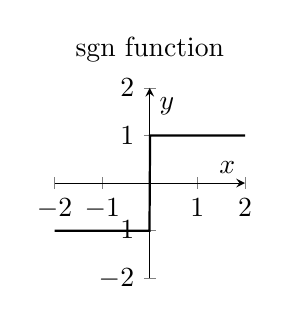
\begin{tikzpicture} 
		\begin{axis} [axis lines=middle, 
			xlabel=$x$,
			ylabel=$y$, 
			xmin=-2,xmax=2,
			ymin=-2, ymax=2,
			%grid=major,
			width=4cm, height=4cm,
			title={sgn function},
			%domain=0:150,
			samples=800] 
			\addplot [thick] {sign x}; 
			%\legend{$Legenda$};
		\end{axis} 
	\end{tikzpicture}
\end{center}

\subsection{Uniqueness}
In order to explain the uniqueness property we look at the following example:
\paragraph{Example} Consider the following ODE: 
\[
\dot{x}(t)=x(t)^{1/3}, x(0)=0.
\]
The solution of this system can be computed and it is not unique, in fact:
\begin{itemize}
	\item $x(t)=0$,
	\item $x(t)=\frac{2}{3}t^{3/2}.$
\end{itemize}
are the two solution of the system.


%% controllare la funzione non è simmetrico il disegno
\begin{center}
	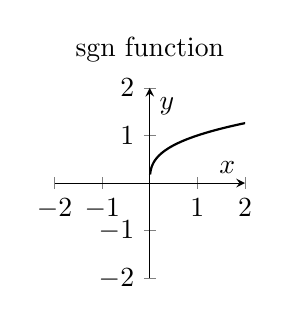
\begin{tikzpicture} 
		\begin{axis} [axis lines=middle, 
			xlabel=$x$,
			ylabel=$y$, 
			xmin=-2,xmax=2,
			ymin=-2, ymax=2,
			%grid=major,
			width=4cm, height=4cm,
			title={sgn function},
			%domain=0:150,
			samples=800] 
			\addplot [thick] {x^(1/3)}; 
			%\legend{$Legenda$};
		\end{axis} 
	\end{tikzpicture}
\end{center}

We have noticed that continuity is not enough for uniqueness, for this reason we have to make a definition:

\begin{defn} [Lipschitz conitinuity]
	$f\colon\Re^n\to\Re^n$ is \emph{Lipschitz continuous}, if in any bounded set A of $\Re^n$ there exist a constant L such that
	\[
	\|f(x_1)-f(x_2)\| \le L \|x1-x_2\|, \forall x_1,x_2 \in A.
	\]
\end{defn}

Given the definition of \emph{Lipschitz continuity} we can state the following theorem:

\begin{thm}[Local existence and uniqueness]
	If $f\colon\Re^n\to\Re^n$ is \emph{Lipschitz continuous}, then $\forall x_0$ there exist a single solution with $x(0)=x_0$ deifned on some $ \left[0,T\right)$.
\end{thm}
But since we are interested in all the time horizon we want to define \emph{global} uniqueness:
\begin{defn} [Lipschitz conitinuity]
	$f\colon\Re^n\to\Re^n$ is \emph{Lipschitz continuous}, if there exist a constant L such that
	\[
	\|f(x_1)-f(x_2)\| \le L \|x1-x_2\|, \forall x_1,x_2 \in \Re^n.
	\]
\end{defn}

Given the definition of \emph{Lipschitz continuity} we can state the following theorem:

\begin{thm}[Local existence and uniqueness]
	If $f\colon\Re^n\to\Re^n$ is \emph{Lipschitz continuous}, then $\forall x_0$ there exist a single solution with $x(0)=x_0$ deifned on $ \left[0,\infty\right)$.
\end{thm}
\paragraph{Example}
Consider the following ODE: 
\[
\dot{x}(t)=-x(t)^2, x(0)=-1.
\]
the solution is $x(t)=\frac{1}{t-1}$ but it is a local solution in $\left[0,1\right)$ since tends to $-\infty$ as $t\to 1$.
\section{Hybrid automaton modelling a hybrid system}
We will introduce this section with an example for describing the main elements of a hybrid automata.
\paragraph{Example} The thermostat
The temperature in a room is controlled by a thermostat which switch a heater on and off.
The dynamics of the temperature x (in $\SI{}{\celsius}$):
\begin{center}
	\begin{itemize}
		
		\item[heater on:] $\dot{x} = -0.2x+6 $ for $(x\to30)$
		\item[heater off:]$\dot{x}= -0.2x $  for $ (x\to 0)$
	\end{itemize} 
\end{center}

\begin{figure}[h]
	\centering
	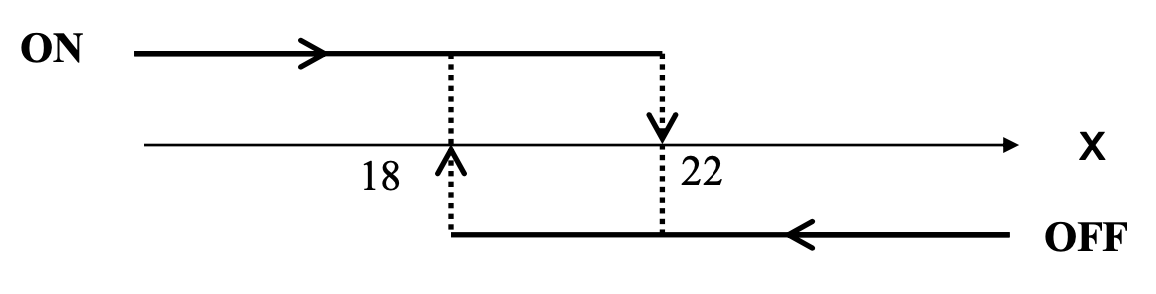
\includegraphics[scale=0.3]{immagini/hyst}
	\caption{Hysteretic Behavior}
	\label{fig:hyst}
\end{figure}

The \emph{goal} is to regulate the temperature around $\SI{20}{\celsius}$. The \emph{strategy} is to turn from OFF to ON the heater as soon as $x\le \SI{18}{\celsius}$ and turn from ON to OFF as soon as $x\ge\SI{22}{\celsius}$.

We have defined to kind of dynamics: the first one of the temperature which is \emph{continuous} and the second one of the heater strategy which is \emph{discrete}. For a better definition of the entire system we can define a \emph{hybrid dynamics} which describe the interleaved continuous and discrete dynamics.

\begin{figure}[h]
	\centering
	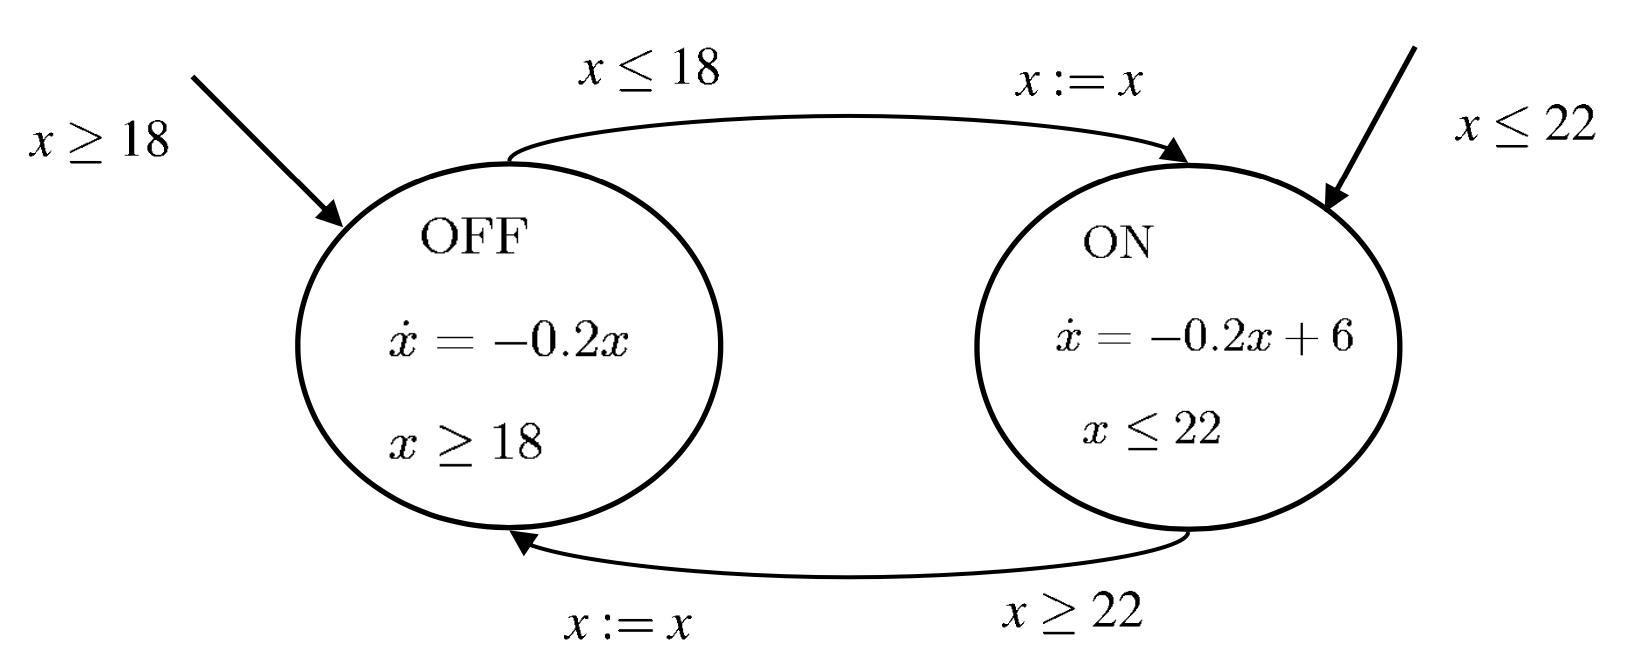
\includegraphics[scale=0.4]{immagini/thermostat}
	\caption{Hybrid dynamics}
	\label{fig:thermostat}
\end{figure}

From the graph we can conclude that e.g in the state ON an evolution can occur untill the temperature reach the boundary of the domain ($x\le22$) and then the guard conditions, if they are respected enable the deterministic transition from ON to OFF.

\subsection{Hybrid Automaton}
A hybrid automaton is a mathematical model for a dynamical system whose state $s =(q,x)$ consists of two components:
\begin{itemize}
	\item continuous state x taking values in $X\in\Re^N$;
	\item discrete state (mode) q taking values in $Q = \left\{q_1,q_2, \dots,q_N\right\}$.
\end{itemize}
Meanwhile an hybrid state space is defined as:
\[
S=Q\times X 
\]
for each value of q, the admissible values for x are only a subset of X.
For example \textcolor{red}{Dom}(q) = \textcolor{red}{domain} for x within the mode q.

The dynamics of q and x are correlated:
\begin{itemize}
	\item x follows an ODE within \textcolor{red}{Dom}(q). The ODE depends on the value of mode q;
	\item q follows a finite automaton with transition triggered by events given by x entering subsets of X called \textcolor{green}{Guards}\\
	\textcolor{green}{$\to G(q,q')$} = values for x enabling the transition from q to q';
	\item when a transition form q to q' takes place, x is reset within Dom(q') by some \textcolor{cyan}{Reset} map\\
	$\to\textcolor{cyan}{R((q,q'),x}$ = reset values for $x^+$ when a transition from q to q' occurs at x.
\end{itemize}
\begin{figure}[th]
	\centering
	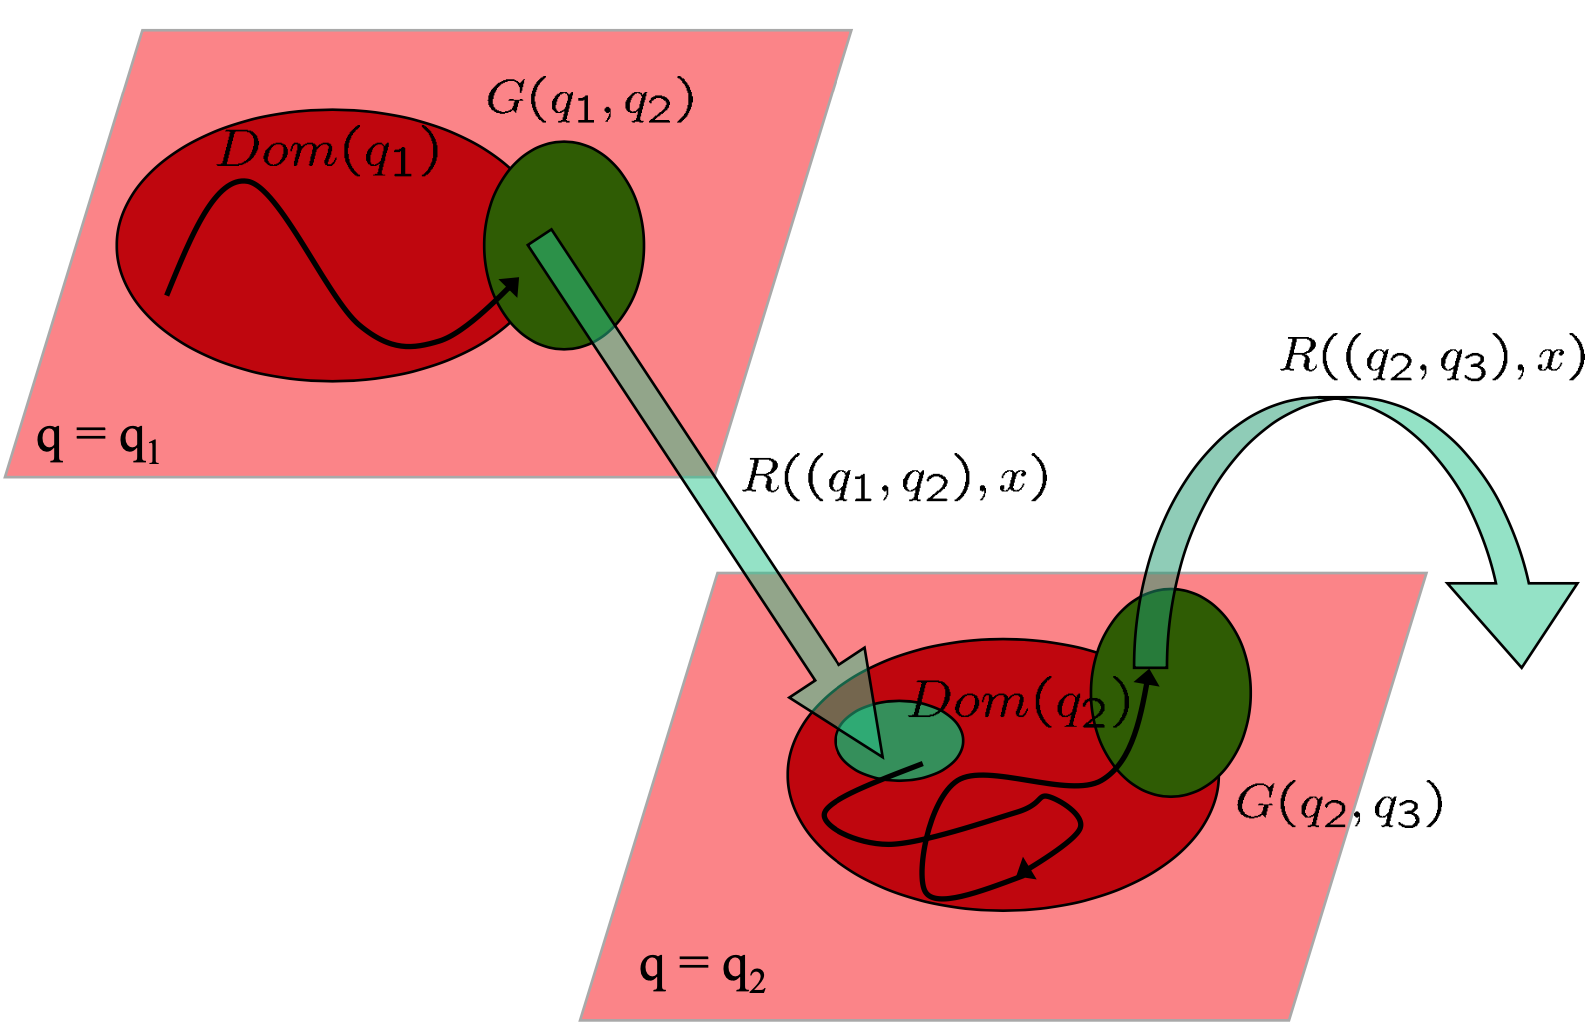
\includegraphics[scale=0.5]{immagini/trans}
	\caption{Combination of continuous evolution (black) and discrete transition (green)}
	\label{fig:trans}
\end{figure}
\subsubsection{Formal definition}
A \textcolor{red}{hybrid automaton} H is a collection H=(Q,X,f\textit{Init},Dom,E,G,R)
\begin{itemize}
	\item $Q = \left\{q_1,q_2, \dots,q_N\right\}$ is a \textcolor{green}{set of discrete states} (modes)
	\item $X=\Re^n$ is the \textcolor{green}{continuous state space}
	\item $f\colon Q\times X\to\Re^n$ is a \textcolor{green}{set of vector fields} on X
	\begin{itemize}
		\item[-] for each $q\in Q,f(q,\cdot)$ is the vector field of the ODE governing the evolution of x
		\item[-] for each $q\in Q,f(q,\cdot)$ is assumed to be \textcolor{red}{globally Lipschitz continuous}
	\end{itemize}
	\item $\emph{Init} \subseteq Q \times X$ is a \textcolor{green}{set of initial states}
	\item $Dom \colon Q \to 2^X$ assigns to each $q\in Q$ a \textcolor{green}{domain} Dom(q) of X
	\item $E \subseteq Q \times Q$ is a \textcolor{green}{set of transitions} (edges)
	\item $G\colon E\to 2^X$ is a \textcolor{green}{set of guards} (guard condition)
	\begin{itemize}
		\item[-] for each e=(q,q'), whenever x reaches G(e) from within Dom(q), transition e is enabled
	\end{itemize}
	\item $R\colon E\times X \to 2^X$ is a \textcolor{green}{set of reset maps}
	\begin{itemize}
		\item[-] for each $e=(q,q') \in E$ and $x \in Dom(q), R(e,x)\subseteq Dom(q')$ is the set of values that x can be reset to after the transition e.
	\end{itemize}
\end{itemize}
\begin{figure}[h]
	\centering
	\includegraphics[scale=0.4]{immagini/scheme}
	\caption{Graphical representation of finite automaton}
	\label{fig:scheme}
\end{figure}

\paragraph{Example}
Coming back to the previous example of the thermostat, referring to Figure \ref{fig:thermostat}, we define mathematically the components H=(Q,X,f\textit{Init},Dom,E,G,R)
\begin{itemize}
	\item $Q=\left\{ON,OFF\right\}$;
	\item $X=\Re$;
	\item $f(OFF,x)=-0.2x$; 
	\item $f(ON,x)=-0.2x+6$;
	\item $\emph{Init}=\left\{(OFF,x)\colon x\ge18\right\} \cup \left\{(ON,x)\colon x\le22\right\}$ 
	\item $Dom(OFF)=\left[18,\infty \right)$
	\item $Dom(ON)=\left(-\infty,22\right]$
	\item $E=\left\{(OFF,ON),(ON,OFF)\right\}$
	\item$G((OFF,ON))=\left(-\infty,18\right]$
	\item$G((OFF,ON))=\left[22,\infty\right)$
	\item$R(e,x)=\left\{x \right\} \forall e \in E$
\end{itemize}
\subsubsection{Execution}
To define an execution of a hybrid system, we need to introduce first the notion of
\begin{itemize}
	\item hybrid time set
	\item hybrid trajectory (which includes hybrid time set among its components)
\end{itemize}

An execution of a hybrid automaton H is a hybrid trajectory that is ''consistent'' with the definition of H.

\paragraph{Hybrid time set} A \textcolor{red}{hybrid time set} is a finite or infinite sequence of intervals $\tau = \left\{I_k,k=0,1\dots,M\right\}$ such that
\begin{itemize}		
	\item$\left[\tau_k,\tau_k'\right] $ for $ k < M$ where $\tau_k$ represent times of discrete transition
	\item$\left[\tau_M,\tau_M'\right]$ or $I_M=\left[\tau_M,\tau_M'\right) $ if $ M<\infty$;
	\item $\tau_k' = \tau_{k+1}$ that means there are no gasp and the intervals are consecutive;
	\item $\tau_k \le \tau_k'$ so intervals can be degenerated to represent multiple transitions at the same time.
\end{itemize}
\begin{figure}[h]
	\centering
	\label{fig:timeset}
	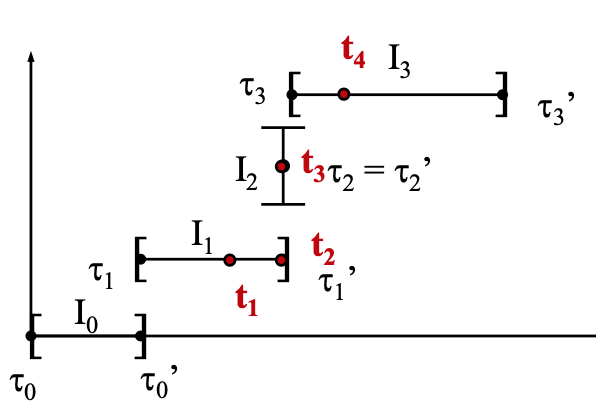
\includegraphics[scale=0.6]{immagini/time_set}
	\caption{Hybrid time set: the elements of $\tau$ are linearly ordered.}
\end{figure}

There are \textcolor{red}{two notion of length} for a hybrid time set $\tau = \left\{I_k, k=0,1,\dots,M\right\}$:
\begin{itemize}
	\item Discrete extent:
	\[<\tau>=M+1 \] that represent \textcolor{red}{number of discrete transition}
	\item Continuous extent:
	\[ \|\tau\|=\sum\limits_{k=1}^M |\tau_k'-\tau_k| \] that represent \textcolor{red}{total duration of intervals in $\tau$}
\end{itemize}
\paragraph{Classification}  Linked to the definition of \emph{length} we can differentiate three different type of time set $\tau = \left\{I_k, k=0,1,\dots,M\right\}$:
\begin{itemize}
	\item Finite: if $<\tau>$ is finite and $I_M=\left[ \tau_M,\tau_M'\right]$;
	\item Infinite: if  $<\tau>$ is infinite or $\|\tau\|$ is infinite;
	\item Zeno: if  $<\tau>$ is infinite but $\|\tau\|$ is finite.
\end{itemize}
\begin{figure}[h]
	\centering
	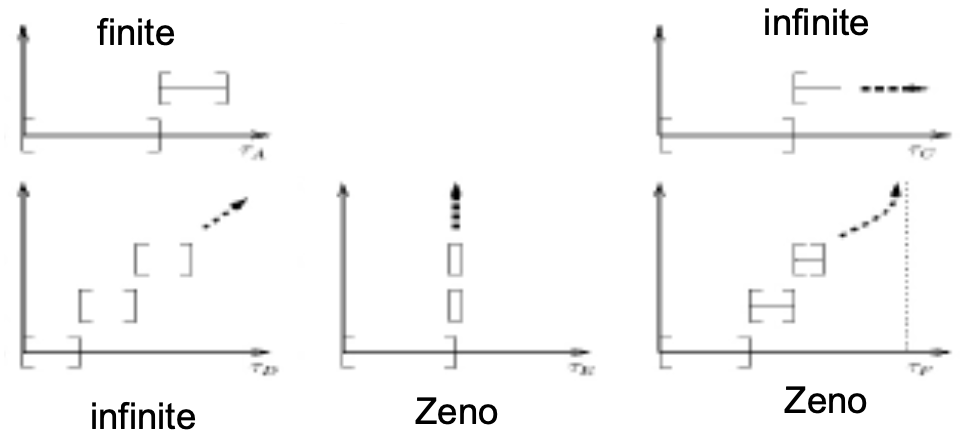
\includegraphics[scale=0.5]{immagini/classification}
	\label{fig:classification}
	\caption{Classification of the time set}
\end{figure}
To complete the fundamentals for defining an \emph{execution} of a hybrid data set we need to treat the hybrid trajectory.
\paragraph{Hybrid trajectory}
A \textcolor{red}{hybrid trajectory} is a triple ($\tau$,q,x) that consist of:
\begin{itemize}
	\item A hybrid time set $\tau = \left\{I_k, k=0,1,\dots,M\right\}$;
	\item Two sequences of functions $q = \left\{q_k(\cdot), k=0,1,\dots,M\right\}$  and $x = \left\{x_k(\cdot, k=0,1,\dots,M\right\}$ such that:
	\begin{itemize}
		\item $q_k\colon I_k\to Q$
		\item $x_k\colon I_k \to X$
	\end{itemize}
\end{itemize}
\begin{remark}
	\begin{enumerate}
		\item this is a mixture of the two notions of continuous and discrete evolution
		\item signals x and q can take multiple values at the same time instant
	\end{enumerate}
\end{remark}

Finally, since we know the concept of hybrid time set and trajectory,  we can define properly an execution:
\begin{defn} 
	A hybrid trajectory ($\tau$,q,x) is an \textcolor{red}{execution (solution) of the hybrid automaton} H=(Q,X,f\textit{Init},Dom,E,G,R) if it satisfies the following conditions:
	\begin{enumerate}
		\item \textcolor{green}{Initial condition:} $(q_0(\tau_0),x_0(\tau_0)\in \emph{Init}$
		\item \textcolor{green}{Continuous evolution:} for all j such taht $\tau_k < \tau_k'$ 
		\begin{itemize}
			\item $q_k\colon I_k\to Q$ is constant
			\item $x_k\colon I_k \to X$ is the solution of the ODE associated with $q_k(\tau_k)$
			\item $x_k(t)\in Dom(q_k(\tau_k)),t\in \left[\tau_k,\tau_k'\right)$
		\end{itemize}
		\item \textcolor{green}{Continuous evolution:} for all j such that $\tau_k < \tau_k'$ 
		\begin{itemize}
			\item $q_k(\tau_k'),q_{k+1}(\tau_{k+1})\in E$ transition is feasible
			\item $x_k(\tau_k')\in G(q_k(\tau_k'),q_{k+1}(\tau_{k+1}$ guard condition satisfied
			\item $x_{k+1}(\tau_{k+1})\in R((q_{k+1}(\tau_{k+1})),x_k(\tau_k')$ reset condition satisfied
		\end{itemize}
	\end{enumerate}
\end{defn}
So now we want analyze that situation in which the execution can go wrong. From the side of problems concerning the ODE solution (like existence, uniqueness, finite escape) we know we are fine thanks to the assumption of Lipschitz global continuity. But problems can arise also due the hybrid nature of the system. The problem we want to analyze are:
\begin{itemize}
	\item Zeno;
	\item chattering;
	\item blocking;
	\item nondeterministic.
\end{itemize}

\subsubsection{Problem and solution of the hybrid execution }
\paragraph{Zeno} Let ($\tau$,q,x) be an execution of H. ($\tau$,q,x)  is called \textcolor{red}{Zeno execution} if $\tau = \left\{I_k, k=0,1,\dots,M\right\}$ is Zeno (infinite number of discrete transition in finite time)\\
\paragraph{Chattering} Let ($\tau$,q,x) be an execution of H. ($\tau$,q,x)  is called \textcolor{red}{chattering execution} if $\tau = \left\{I_k, k=0,1,\dots,M\right\}$ is Zeno (infinte number of discrete transition in finite time and after some $h \ge 0$, all the intervals $I_k,k \ge h$, are singletons.\\
In practice this means that after a certain time instant the continuous transition remains constant while the discrete transitions occurs infinite times in a finite time set.\\
A possible solution of this problem is called \textbf{temporal regularization} and consist to add a sort of delay between two discrete transition such that we avoid infinite number of discrete transition in finite time. 
\paragraph{Example}[The Bouncing Ball]
We want to analyze the situation of a ball bouncing along vertical axis freely. We can identify two situations: ball flying in the air and ball hitting the ground. The state of the system are the position $x_1$ and the velocity $x_2$. In Figure
\begin{figure}[h]
	\centering
	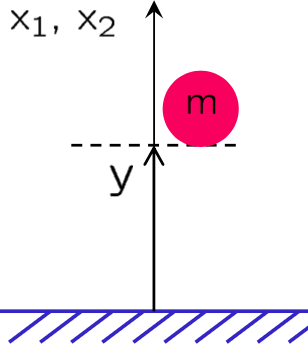
\includegraphics[scale=0.4]{immagini/bouncing ball}
	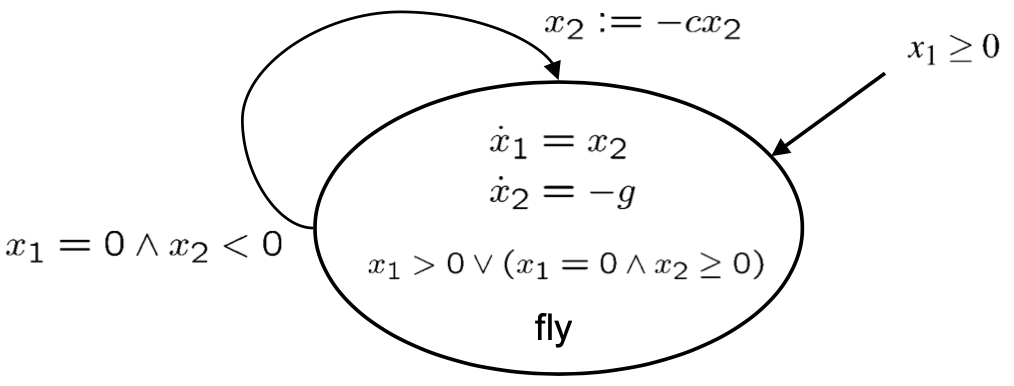
\includegraphics[scale=0.4]{immagini/bb_automata}
	\caption{Bouncing ball model}
	\label{fig:bbautomata}
\end{figure}
The mathematical description of the components H=(Q,X,f\textit{Init},Dom,E,G,R) is:
\begin{itemize}
	\item $Q=\left\{fly\right\}$;
	\item $X=\Re^2$;
	\item $f(fly,x)=[x_2,-g]^T$; 
	\item $\emph{Init}=\left\{(fly,(x_1,x_2))\colon x_1\ge0\right\}$ 
	\item $Dom(fly)=\left\{(x_1,x_2)\colon x_1>0\right\} \cup \left\{(x_1,x_2)\colon x_1= 0, x_2\ge 0 \right\}$;
	\item $E=\left\{(fly,fly)\right\}$
	\item$G((fly,fly))=\left\{(x_1,x_2)\colon x_1= 0, x_2<0 \right\}$
	\item$R(e,(x_1,x_2))=\left\{(x_1,-cx_2) \right\} \forall e \in E$
\end{itemize}
Since for $x_1(0)=0, x_2(0)>0$ occurs infinite number of transitions in finite time this is a \textcolor{red}{Zeno} hybrid system.
Implementing the possible solution we have described before we obtain the following diagram associated to the following evolution of the states.
\begin{figure}[h]
	\centering
	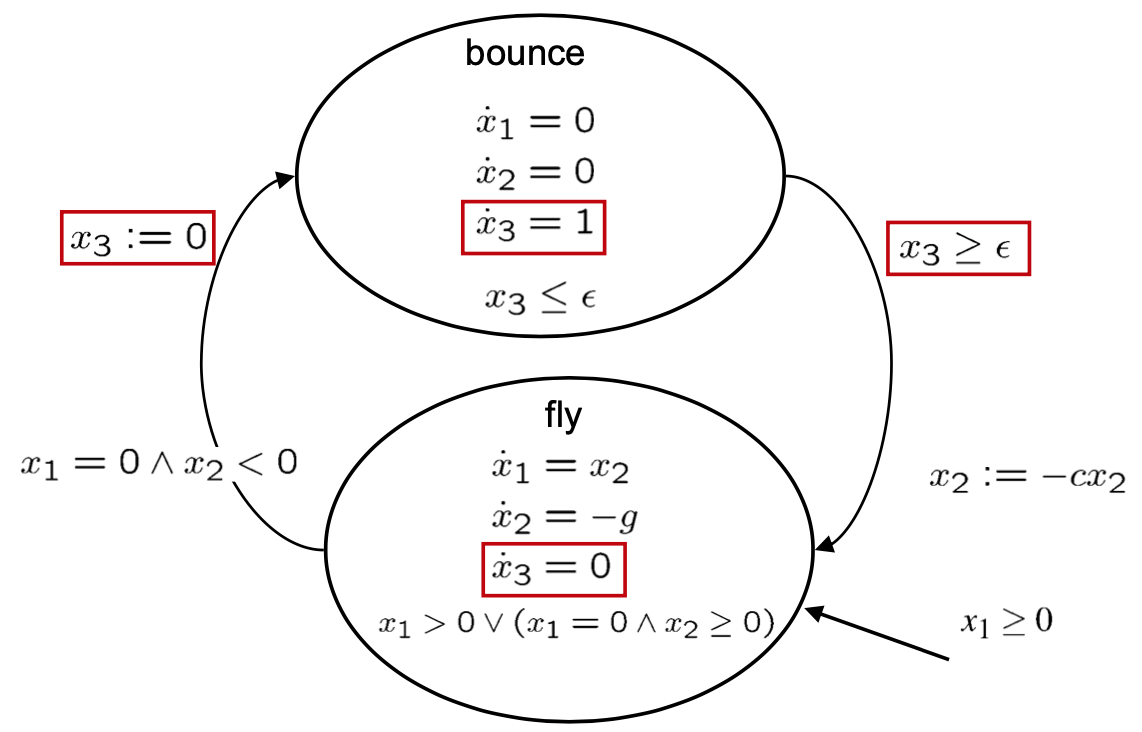
\includegraphics[scale=0.3]{immagini/corrected_bb_automata}
	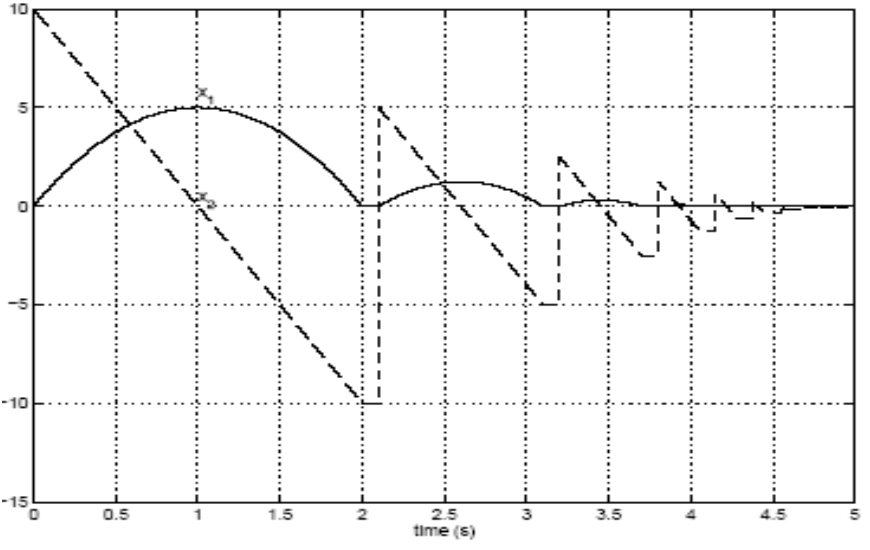
\includegraphics[scale=0.3]{immagini/evolution_bb}
	\caption{Correction of Zeno system with temporal delay equal to 0.1}
	\label{fig:bbautomata_corrected}
\end{figure}
Let's now treat the last two problems: the blocking system and the nondeterministic.
\subsubsection{Blocking vs Non-Blocking}
A \textcolor{red}{hybrid automaton} H=(Q,X,f\textit{Init},Dom,E,G,) is \textcolor{red}{non-blocking} if for all initial states $(q,x) \in \emph(Init)$ there is an infinite execution starting at (q,x).
\begin{remark}
In practice this is only a \textbf{sufficient condition} because there can be a condition that if it is reached the system blocks but it is not mandatory that this condition is reached.
\end{remark}
Let's give now a formal definition of this concept.
\begin{defn}
	Given a hybrid automaton  H=(Q,X,f\textit{Init},Dom,E,G,R), \textcolor{red}{transition states} are those states from which continuous evolution is impossible:
	\[
	Trans:=\left\{(q',x')\in Q\times X\colon \forall \delta>0,\exists t \in[0,\delta] \text{such that} \, x(t)\notin Dom(q')\right\}
	\] where x(t) is the solution of $\frac{dx}{dt}=f(q',x) \text{with} \, x(0)=x'$.
\end{defn}
\begin{tcolorbox}
	A hybrid automaton is non-blocking if:
	\begin{enumerate}
		\item $f(q,\cdot)$ is globally Lipschitz for each $q\in Q$;
		\item for eah $(q,x)\in Trans$, there exists q' such that $(q,q')\in E$ and $x \in G(q,q')$ 
	\end{enumerate}
\end{tcolorbox}
\paragraph{Example}
Let's look at the automata in Figure \ref{fig:non-blocking}:
considering the following state$\left\{(q_2,x)\colon x\le 0\right\} \subseteq Trans$ we notice that is trivial fo $x<0$ because the continuous state is outside $Dom(q_2)$, so for $x=0$ it would exit domain. Even if  there are no discrete transition possible from $q_2$ it is still non blocking because for all initial states $(q,x)\in Init$ there is an infinite execution starting at (q,x).
\begin{figure}[h]
	\centering
	\includegraphics[scale=0.4]{"immagini/non blocking"}
	\caption{Non blocking hybrid automata}
	\label{fig:non-blocking}
\end{figure}
\subsubsection{Deterministic vs Nondeterministic}
\begin{defn}{Maximal execution}
	An execution is maximal if \emph{it cannot be extended any further}.
\end{defn}
A \textcolor{red}{hybrid automaton} H=(Q,X,f\textit{Init},Dom,E,G,) is \textcolor{red}{deterministic} if for all initial states $(q,x) \in \emph(Init)$ there exists \textcolor{red}{at most one maximal execution} starting at (q,x).\\
But concretely what does cause non determinism?

\begin{SCfigure}[][h]
	\centering
	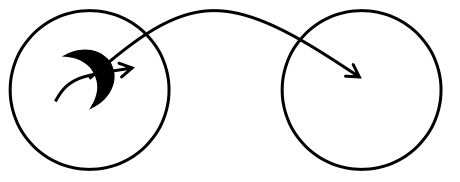
\includegraphics[scale=0.35]{immagini/nd_1}
	\caption{choice between continuous evolution and discrete transitions}
	\label{fig:nd_1}
\end{SCfigure}
\begin{SCfigure}[][h]	
	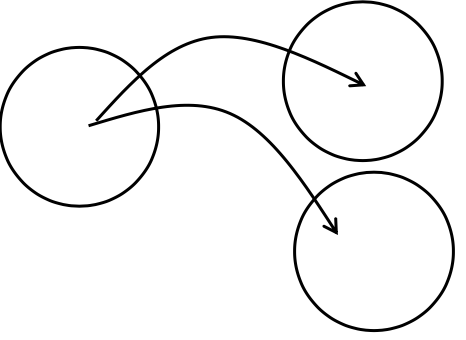
\includegraphics[scale=0.35]{immagini/nd_2}
	\caption{Discrete transitions to multiple modes are jointly enabled}
	\label{fig:nd_2}
\end{SCfigure}
\begin{SCfigure}[][!h]	
	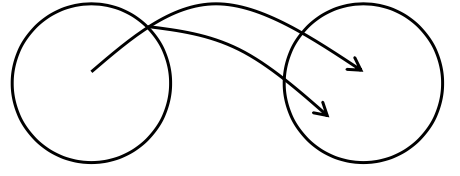
\includegraphics[scale=0.35]{immagini/nd_3}
	\caption{multiple reset positions}
	\label{fig:nd_3}
\end{SCfigure}
 Finally we can summarize the definition if \emph{deterministic} as follow: 
\begin{tcolorbox}
	A hybrid automaton is non-blocking if:
	\begin{enumerate}
		\item a discrete transitions occur only when continuous evolution is not possible;
		\item o multiple discrete transitions are possible at the same time;
		\item there is only one reset position when taking a discrete transition.
	\end{enumerate}
\end{tcolorbox}
\subsubsection{Existence and uniqueness if executions}
A hybrid automaton has a \textcolor{red}{unique infinite execution for each initial state if it is non-blocking and deterministic}.\\
\\
This is a sufficient condition given by  putting together the \textcolor{red}{sufficient conditions for the hybrid automaton to be non- blocking and deterministic}.\\
Formally speaking the conclusion of this section can be summarized like that:
\begin{tcolorbox}
	A hybrid automaton has a \textcolor{red}{unique infinite execution} for each initial state if
	\begin{enumerate}
		\item $f(q,\cdot)$ is globally Lipschitz for each $q\in Q$;
		\item for eah $(q,x)\in Trans$, there exists q' such that $(q,q')\in E$ and $x \in G(q,q')$ \\ \emph{(a discrete transition should be possible from the Trans states)
		}
		\item If $x \in G(q,q')$ for some $(q,q') in E$, then $(q,x) \in Trans$\\ \emph{(discrete transitions occur only when continuous evolution is not possible)}
		\item If $(q,q'),(q,q'')\in E$, then $G(q,q')\cap G(q,q'')=\emptyset$ \\ \emph{(no multiple discrete transitions are possible at the same time)}
		\item If $(q,q')\in E$ and $x\in G(q,q')$, then $R((q,q'),x)$ is a singleton\\ \emph{(only one reset position when taking a discrete transition)}
	\end{enumerate}
\end{tcolorbox}

%%%% Fine capitolo 1%%%%%
	\pagebreak
	\chapter{Switched system and stability}
\section{Introduction}
What is a switched system? A switched system is the composition of a \emph{family of system} $\dot{x}=f_q(x), q \in Q=\left\{1,2,\dots,m\right\}$ and a signal $\sigma$ that orchestrate the switching of them.\\
\begin{figure}[H]
	\centering
	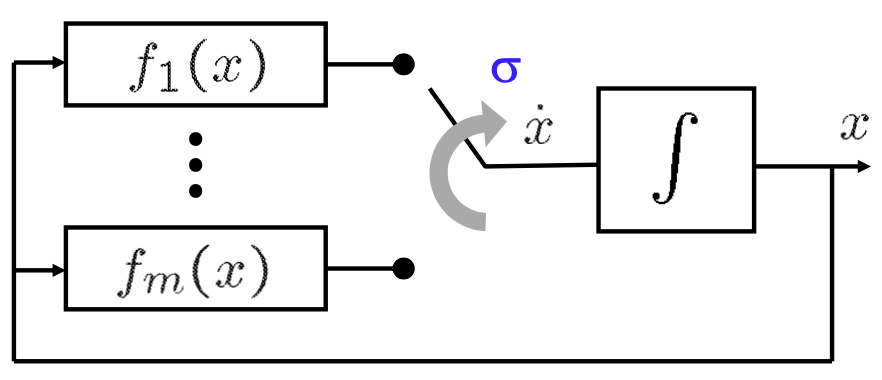
\includegraphics[width=0.7\linewidth]{immagini/swithced_1}
	\caption{Switched system}
	\label{fig:swithced1}
\end{figure}
A switched system can be compared to an hybrid system where the discrete transition mechanism (domains and guards) depends on the switching signal which can be state-dependent or time-dependent.
\begin{figure}[H]
	\centering
	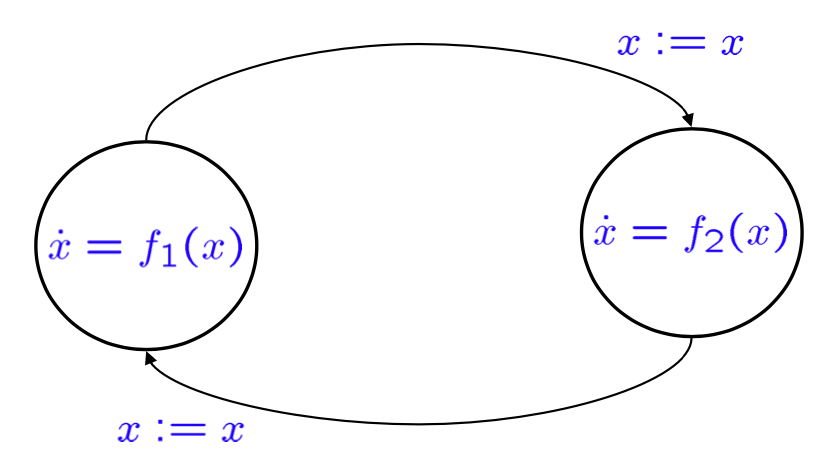
\includegraphics[width=0.7\linewidth]{immagini/swtich_hyb}
	\caption{$\dot{x}=f_{\sigma}(x), \sigma \in Q=\left\{1,2\right\}$}
	\label{fig:swtichhyb}
\end{figure}
\paragraph{State dependent switching example} The state space X is partitioned into operating regions, each one associated to the system is in action in that moment.  The system in action is specified by the switching system $\sigma(x)$.
\begin{figure}[H]
	\centering
	\includegraphics[scale=0.4]{immagini/state_d_sw}
	\caption{State-dependent}
	\label{fig:statedsw}
\end{figure}
\subparagraph{Example} Here is reported an example of a switched linear system.
\begin{figure}[H]
	\centering
	\includegraphics[scale=0.4]{immagini/s_l_S}
	\includegraphics[scale=0.4]{immagini/sls_2}
	\caption{Switching Linear System}
	\label{fig:sls2}
\end{figure}
The hybrid time set of the system in analysis is the following H=(Q,X,f,\textit{Init},Dom,E,G,R):
\begin{itemize}
	\item $Q=\left\{q_1,q_2\right\}$;
	\item $X=\Re^2$;
	\item $f(q_1,x)=A_1x$ and $f(q_2,x)=A_2x$; 
	\item $\emph{Init}=Q \times X$ 
	\item $Dom(q_1)=\left\{(x\in X\colon Cx>0\right\} $ and $Dom(q_2)=\left\{(x\in X\colon Cx\le0\right\} $;
	\item $E=\left\{(q_1,q_2),(q_2,q_1)\right\}$;
	\item$G((q_1,q_2))=\left\{(x\in X\colon Cx\le0\right\} $ and $G((q_2,q_1))=\left\{(x\in X\colon Cx>0\right\} $;
	\item$R((q_1,q_2),x)=R((q_2,q_1),x)=\left\{x \right\}$
\end{itemize}
\paragraph{Time dependent switching example} 
Meanwhile in time dependent switching system the \textcolor{red}{(exogenous) switching signal} is a piecewise constant function on time defined as $\sigma \colon \left[0,\infty\right) \to Q$. $\sigma(t)$ specifies the system that is active at time t.
\begin{figure}[H]
	\centering
	\includegraphics[scale=0.4]{immagini/s_td_s}
	\caption{$\dot{x}=f_{\sigma}(x), \sigma \colon \left[0,\infty\right) \to Q$} 
	\label{fig:stds}
\end{figure}
If the switching signal is abitrary (discrete transition method not specified), then H=(Q,X,f,\textit{Init},Dom,E,G,R):
 \begin{itemize}
	\item $Q=\left\{q_1,q_2\right\}$;
	\item $X=\Re^2$;
	\item $\emph{Init}=Q \times X$ 
	\item $f(q_1,x)=f_1(x)$ and $f(q_2,x)=f_2(x)$; 
	\item $Dom(q_1)=Dom(q_2)=X$;
	\item $E=\left\{(q_1,q_2),(q_2,q_1)\right\}$;
	\item$G((q_1,q_2))=G((q_2,q_1))=X$;
	\item$R((q_1,q_2),x)=R((q_2,q_1),x)=\left\{x \right\}$
\end{itemize}
In conclusion switched system with time-dependent arbitrary switching can be seen as a \textcolor{green}{higher-level abstraction of hybrid automata} where the discrete transition mechanism is not specified.
\subsection{Introduction to stability} \label{introstab}
We want now to start reasoning about the stability of a switched system and thus we need to define what is an equilibrium.
\begin{defn}[Equilibrium]
	Given a family of systems $\dot{x}=f_q(x), q\in Q=\left\{1,2,\dots,m\right\}$ with $f_q(0)=0, \forall q \in Q$: x=0 is an \textcolor{red}{equilibrium} of the switched system.
\end{defn}
Now it's important to study the stability of the equilibrium. Suppose to have a set of system with cardinality equal to two $\dot{x}=A_{\sigma}x$ where $\Re\left\{eigA_{\sigma}\right\}<0, \forall \sigma$ as shown in Figure \ref{fig:12stable} the two independent system are asymptotically stable.
\begin{figure}[H]
	\centering
	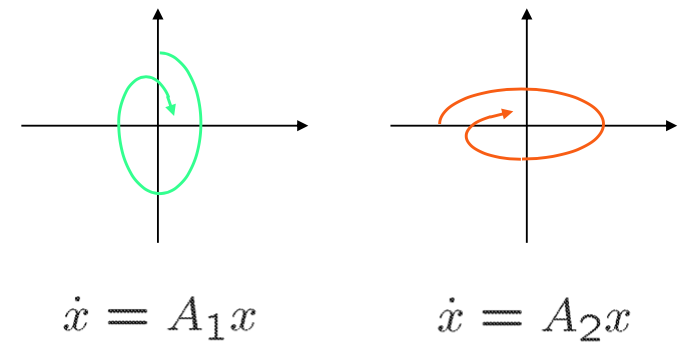
\includegraphics[scale=0.4]{immagini/1_2_stable}
	\caption{Stable trajectories}
	\label{fig:12stable}
\end{figure}
But depending on the switching signals we chose we can have different stability results, even instability of the overall switched system. Let's look what happens with the following example in Figure \ref{fig:12stable}
\begin{figure}[H]
	\centering
	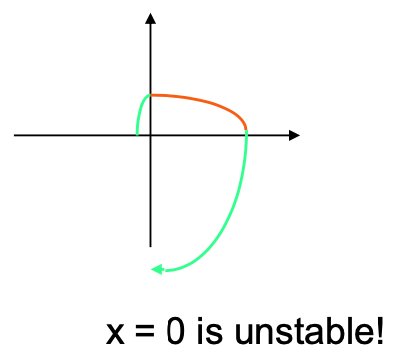
\includegraphics[scale=0.4]{immagini/sw_unstable}
	\includegraphics[scale=0.4]{immagini/sw_ast}
	\caption{Effect of the switching signal on stability}
	\label{fig:swunstable}
\end{figure}
Furthermore, some times even if we have a system of the set which is unstable the overall system can be asymptotically stable if the proper switching signal is chosen (or designed). An example follows in Figure \ref{fig:unst}
\begin{figure}[H]
	\centering
	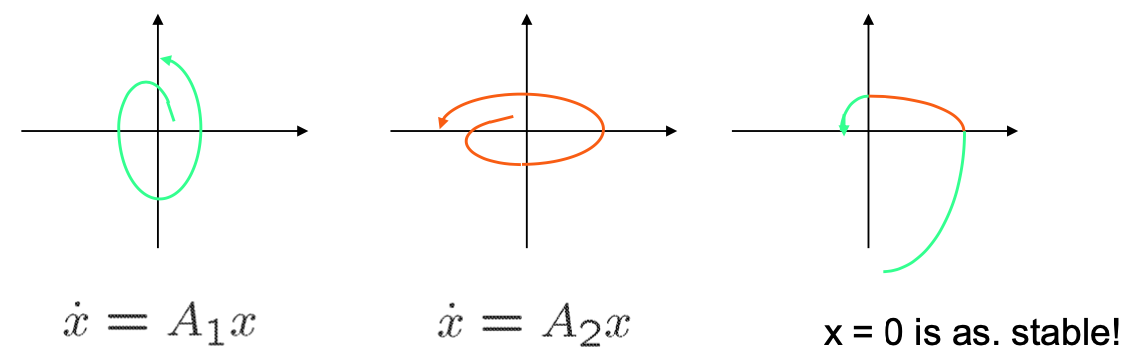
\includegraphics[scale=0.4]{immagini/un+st}
	\caption{Stabilizing with the switching signal}
	\label{fig:unst}
\end{figure}
\section{Stability for arbitrary switching}\label{stab-arb-sw}
In this section we will talk about how to reach global uniform asymptotic stability but before we have to give some definitions and theorems.

\begin{defn}[Globally uniformly asymptotically stable equilibrium]
	The equilibrium x=0 is \textcolor{green}{GUAS} if it is GAS, uniformly with respect to the switching signals $\sigma$.
\end{defn}
A \textcolor{green}{necessary condition for x=0 to be GUAS} is that $\dot{x}=f_q(x), q\in Q=\left\{1,2,\dots,m\right\}$ is a family of systems with GAS equilibrium in x=0.

\begin{defn}
	The family of systems $\dot{x}=f_q(x), q\in Q=\left\{1,2,\dots,m\right\}$ share a \textcolor{green}{common Lyapunov Function} at x=0 if there exists a continuously differentiable ($C^1$) function $V\colon\Re^n\to\Re$ such that \[
	 V(x)>0, \forall x \neq0, V(0)=0\quad \text{and} \quad \frac{\delta V}{\delta x}(x)f_q(x)<0, \forall x \neq0, \forall q \in Q
	 .\]
	 A common Lyapunov function at $x=0$ is quadratic if it is given by $V(x)=x^TPx$ with P symmetric and positive definite.
\end{defn}
\begin{thm}[Common Lyapunov function]\label{lyap-th}
	If the family of systems $\dot{x}=f_q(x), q\in Q=\left\{1,2,\dots,m\right\}$ share a \textcolor{red}{radially unbounded common Lyapunov function} $V\colon\Re^n\to\Re$ at x=0, then, the equilibrium x=0 is GUAS.
\end{thm}
\begin{thm}[Common \emph{quadratic} Lyapunov function] \label{quad-lyap-th}
	If there exists $P=P^T>0$ such that $PA_q+A_q^TP<0, \forall q \in Q= \left\{1,2,\dots,m\right\}$ then the equilibrium x=0 is GUAS.
\end{thm}
\begin{proof}
	$V(x)=x^TPx$ is radially unbounded common Lyapunov function at x=0.
\end{proof}
\begin{remark}
	The existence of a globally quadratic Lyapunov function is not necessary for x=0 to be GUAS.
\end{remark}

%%%5 there is an example but i need to listen the lesson%%%%
\subsection{Switched linear system with a special structure}
We now focus on a specific set of switched linear (the family of possible dynamics is linear) system which are characterized by matrices $A_q,\,q\in Q=\left\{1,2,\dots,m\right\}$ which are Hurwitz and:
\begin{itemize}
	\item commute
	\item are upper or lower triangular
\end{itemize}
\subsubsection{Commuting matrices}
So, considering, for example, for simplicity the case of $Q=\left\{1,2\right\}$ system defined by $\dot{x}=A_{\sigma}x$. Calling $s_k$ the time interval where $\sigma=1$ is activated and $t_k$ when $\sigma=2$ is activated the evolution of x(t) can be found thanks to Lagrange formula for each one dynamics.
\begin{figure}[H]
	\centering
	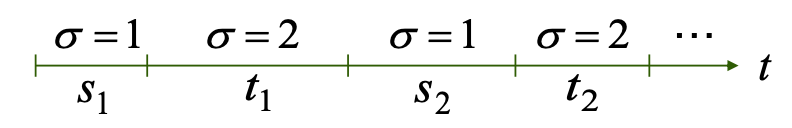
\includegraphics[scale=0.4]{immagini/bho}
	\caption{Arbitrary activation sequency}
	\label{fig:bho}
\end{figure}
\[
x(t)=e^{A_2t_k}e^{A_1s_k}\dots e^{A_2t_1}e^{A_1s_1}x(0)=e^{A_2(t_k+\dots +t_1)}e^{A_1(s_k+\dots +s_1)}x(0)\to 0
\] as $t\to\infty$.
We can also \textbf{prove the stability} building a common quadratic Lyapunov function. We firstly build a matrix $P_1$ which satisifies the Lyapunov equation and then plug in $P_1$ as the righten side of another Lyapunov equation in order to find $P_2$. So my statement is that $P_2$ build in such a way is the common quadratic Lyapunov function for the two linear system, one characterized by matrix $A_1$ and the other by matrix $A_2$.
\[
P_1A_1+A_1^TP_1=-I\]
\[
P_2A_2+A_2^TP_2=-P1
\]
So we can formalize as follow: $\exists\ a \ quadratic \ common \ Lyapunov \ function: V(x)=x^TP_2x$.First of all we know that if $A_1$ is Hurwitz there is an unique positive definite solution to the first Lyapunov equation which is $P_1$ and when we plug in $P_1$ in the second equation the same consideration apllies because also $A_2$ is Hurwitz. Where $P_1$ and $P_2$ are as follows:
\[P_2=\int_{0}^{\infty} e^{A_2^Tt}P_1e^{A_2^Tt}\, dt \qquad P_1=\int_{0}^{\infty} e^{A_1^Tt}Ie^{A_1^Tt}\, dt\]
Now plugging in the first expression in the second, and commuting the exponential (to be clear, switching $A_1$ and $A_2$) one we obtain: 
\[P_2=\int_{0}^{\infty} e^{A_1^T\tau}\underbrace{\int_{0}^{\infty} e^{A_2^Tt}Ie^{A_2^Tt}\, dt}_{Q}e^{A_1^T\tau}\, d\tau
\]
And so we can notice that $P_2$ satisfies also the following Lyapunov equation for the dynamic $A_1$:
\[
P_2A_1+A_1^TP_2=-Q.
\]
\subsubsection{Triangular Hurwitz matrices}
	\[
	\dot{x}_1=\lambda_{1,\sigma}x_1+a_{\sigma}x_2\]
	\[
	\dot{x}_!=\lambda_{2,\sigma}x_2
	\]
We know that the two $\lambda$ since the matrices are Hurwitz should be strictly negative. We notice that the second equation is independent from the first one so we can compute the evolution of $x_2(t)$ as we did in the previous chapter. So we know that $x_2(t)$ is the product of many exponential but the exponentials of a scalar which are indeed the eigenvalues $\lambda$. Thus when I found an upper bound I can say that the absolute value of $x_2(t)$ is less or equal to the exponential with the lowest rate of decrease which is the one associated to the large eigenvalue among every dynamics eigenvalues. In conclusion $x_2(t)$ goes to zero because all eigenvalue are strictly negative.
\[
\dot{x}_2=\lambda_{2,\sigma}x_2 \Rightarrow \left|x_2(t)\right|\le e^{\max_p\lambda_{2,p}t}\left |x_2(0)\right| \to 0
\]
\[
\boxed{\dot{x}_1=\lambda_{1,\sigma}x_1}+\boxed{a_{\sigma}x_2}\Rightarrow x_1(t)\to 0
\]
The same thing can be said for the first equation. Here $x_2(t)$ can see as an input that goes to zero. The first part is an \underline{exponentially stable system} while the second part is, as we demonstrated previously, a \underline{exponentially decaying perturbation} so tends to zero as t tends to infinity.

\section{Stability for constrained switching}
The main difference between arbitrary and constrained switching is that now we can select the way we switch from one dynamic to the other  in such a way we get global asymptotical stability for the zero equilibrium. Notice that we can't get anymore uniform stability.
\subsection{Stability under slow switching}
Supposing to have a linear system, (can be extended to nonlinear) the matrices we are given are Hurwitz but as we saw in \ref{introstab} even if the matrices are Hurwitz we are not guarantied of the preserving of stability. So the idea here goes as follow: if each dynamic is asymptotically stable, if you stay long enough with one dynamic activated you are going to have a contraction of the value of the state x(t) because, eventually, as the time goes to infinity the state will tend to zero. So at this point if we initialize the absolute value of $\left\|x(0)\right\|$ at a certain value if we wait enough, before switching to the other dynamic, (because there can be overshoots) the absolute value $\left\|x(t)\right\|$ will become smaller then $\left\|x(0)\right\|$). This waiting time is called \textbf{dwell time} $\tau_D$. So the choice of $\tau_D$ is crucial for the preservation of global asymptotic stability. Let's prove it more formally.
Starting from the computation of $x_(t)$ as we did before:
\[x(t)=e^{A_2t_k}e^{A_1s_k}\dots e^{A_2t_1}e^{A_1s_1}x(0)\]
and applying the absolute value to both sides, the relation still holds:
\[\|x(t)\|=\|e^{A_2t_k}e^{A_1s_k}\dots e^{A_2t_1}e^{A_1s_1}x(0)\|.\]
Now the idea is to upper bound this expression with the product of the norm of the exponentials of the matrices:
\[\|x(t)\| \le \| e^{A_2t_k}\| \|e^{A_1s_k}\dots e^{A_2t_1}e^{A_1s_1}x(0)\|.\]
This is possible thanks to the definition of the norm which I'm recalling here:
\begin{defn}[Norm] \label{norm}
	\[\|M\| = \sup_{y \neq0}\frac{\|My\|}{\|y\|}\to \|My\| \le \|M\|\|y\|
	\]
\end{defn}
And iterating the procedure we finish into:
\[\|x(t)\| \le \| e^{A_2t_k}\| \|e^{A_1s_k}\|\dots \|e^{A_2t_1}\|\|e^{A_1s_1}\|\|x(0)\|.\]
So, again applying the Definition \ref{norm}, we have:
\begin{equation}\label{eq1}
	\|e^{At}\|=\sup_{x_0 \neq0}\frac{\|e^{At}x_0\|}{\|x_0\|}\le \mu e^{-\lambda_0t},t \ge 0
\end{equation}
Where this $\lambda_0$ is a positive number that has to be smaller then the minimum absolute value of the real part of all eigenvalues. This is the \emph{lowest decay rate} so that the inequality holds for all dynamics.
How can I chose given all this information $\tau_D$? 
\begin{equation} \label{eq2}
	\tau_D \ge \frac{\log\mu}{\lambda_0-\lambda} \text{ with } \lambda\in(0,\lambda_0)\Longrightarrow \mu \le e^{\tau_D(\lambda_0-\lambda)}
\end{equation}

So now plugging the expression of $\mu$ found in \ref{eq2} in \ref{eq1} we obtain:
\begin{equation} \label{eq3}
	\|e^{A_i\Delta t}\| \le \mu e^{-\lambda_0\Delta t}\le e^{\tau_D(\lambda_0-\lambda)}e^{-\lambda_0\Delta t}
\end{equation}
and since $\Delta t \ge \tau_D$ and $\lambda_0 > \lambda$ we can upperbound and simplify as follow:
\begin{equation}
 		\|e^{A_i\Delta t}\| \le \mu e^{-\lambda_0\Delta t}\le e^{\tau_D(\lambda_0-\lambda)}e^{-\lambda_0\Delta t} \le e^{\Delta t(\lambda_0-\lambda)}e^{-\lambda_0\Delta t}=\boxed{e^{-\lambda t}\|x(0)\|}
\end{equation}
Here $\lambda_0$ is the \textbf{exponential rate of convergence} and should not be higher then maximum eig(A-LC). So we not only have global asymptotic stability but also \textbf{global exponential stability}.
\begin{remark}
	$\tau_D$ can be tailored to each time interval associated to each single dynamic independently.
\end{remark}
\section{Stability under state-dependent switching}
If since now we have studied the stability property of a time-dependent switching system, in this section we will show some result on how to prove or enforce stability of a state-dependent switching system.
\linebreak[2]
\begin{figure}[H]
	\centering
	\includegraphics[scale=0.4]{immagini/ss-ds}
	\caption{State-dependent switching system in the partitioned state space}
	\label{fig:ss-ds}
\end{figure}
Suppose we have given a switching rule and the partition of state space as in section \ref{fig:ss-ds}. In every part of the state space we have an associated dynamic. How can we prove the stability of the zero equilibrium? We start exploiting the following notion of state-dependent common Lyapunov function.
\begin{defn}[state-dependent common Lyapunov function]
	The family of systems $\dot{x}=f_q(x), x \in \Re^n, q \in Q=\left\{1,1,\dots,m\right\}$ has a \textcolor{green}{state-dependent common Lyapunov function} at x=0 if there exists a $C^1$ function $V\colon \Re^n\to\Re$ such that
	\[
	V(x)>0, \forall x\neq 0, V(0)=0	
		, \forall x \in \Re^n
	\]
	where $\sigma\colon X \to Q$.
\end{defn}

 We can notice that this is a less strict requirement then the one of common quadratic Lyapunov function stated in Theorem \ref{quad-lyap-th}. Why? Here the dynamic should decrease only in the state space region in which is activated. For example in figure \ref{fig:ss-ds} the function $f_1(x)$ is not required to be decreasing when we are in $X_3$.\\
 A theorem can be derived:
\begin{thm}
	Given the system $\dot{x}=f_{\sigma}(x), \sigma\colon X\to Q$, if there exists a radially unbounded state-dependent common Lyapunov equation at x=0 for the switched system, then, the equilibrium x=0 is GAS.
\end{thm}
\begin{remark}
	need that $\frac{\delta V}{\delta x}(x)f_{\sigma(x)}(x)<0$ only when $\sigma$ is equal to q. So in the switched linear case matrices $A_q$ are not required to be Hurwitz.
\end{remark}
\subsection{Stabilization by switching}
It is possible given two (or more) unstable linear system to build a state dependent switching rule that makes the zero equilibrium GAS. The trick is basically to build a state-dependent switching rule such that there exists a common Lyapunov function for this two dynamics of the system.\\ This is possible if:
\begin{thm}
	If the matrices $A_1$ and $A_2$ have a convex Hurwitz combination, then, there exists a state-dependent switching strategy such that the equilibrium x=0 of the switching system $\dot{x}=A_{\sigma(x)}x$ is GAS.
\end{thm}

But what does it mean \emph{convex combination}? Let's do an example:
\paragraph{Example} Considering $\dot{x}=A_1x$ and $\dot{x}=A_2x$ both unstable, assume:
\[
A=\alpha A_1+(1-\alpha)A_2 \text{ Hurwitz for some } \alpha \in (0,1)
\]
This is a \emph{convex} combination because the selected parameters are between zero and one and sum up to one. Since A is Hurwitz there exists a matrix P such that Lyapunov inequality is satisfied
\[
A^TP+PA<0.
\]
Now we put in place of A the first expression defined as an assumption:
\[
\alpha(A_1^TP+PA_1)+(1-\alpha)(A_2^TP+PA_2)<0
\]so for each $x\neq0$ either
\[
\underbrace{x^T(A_1^TP+PA_1)x<0}_{\text{define region $X_1$ where system 1 is active}} \ \textbf{or} \ \underbrace{x^T(A_2^TP+PA_2)x<0}_{\text{define region $X_2$ where system 2 is active}}
\]
We notice that the above inequality come from the derivative of the Lyapunov function $V(x)=x^TPx$ along the two dynamics. So we activate the dynamic when V decreases. So practically we enforce V(x) to be a common quadratic Lyapunov function.
$V(x)=x^TPx$ is a radially unbounded state-dependent common Lyapunov function at x=0 for $\dot{x}=A_{\sigma(x)}x$ $\Longrightarrow$ x=0 is GAS.
In conclusion: what is the shape of this two regions? There are conic regions because for example taking a random point in yellow region, every point on the line that pass trough the point and the origin satisfies the same inequality because they can be parametrized  as a function of $\bar{x}$ as $K\bar{x}$ and if we put $K\bar{x}$ in the fuction above we get $K^2$ that multiplies the other part of the expression and doesn't change the sign of it.
\begin{figure}[H]
	\centering
	\includegraphics[scale=0.4]{"immagini/conic regions"}
	\caption{$X_1$ is the yellow region, $X_2$ is the green one.}
	\label{fig:conic-regions}
\end{figure}
Notice that the two parts partially overlap because they can't be just complementary because the boundary cannot belong to any region (strict inequality) so they should overlap at least a bit.
\section{Observer design}
The goal of an observer is to recover the state of a system from its input and output.\begin{figure}[H]
	\centering
	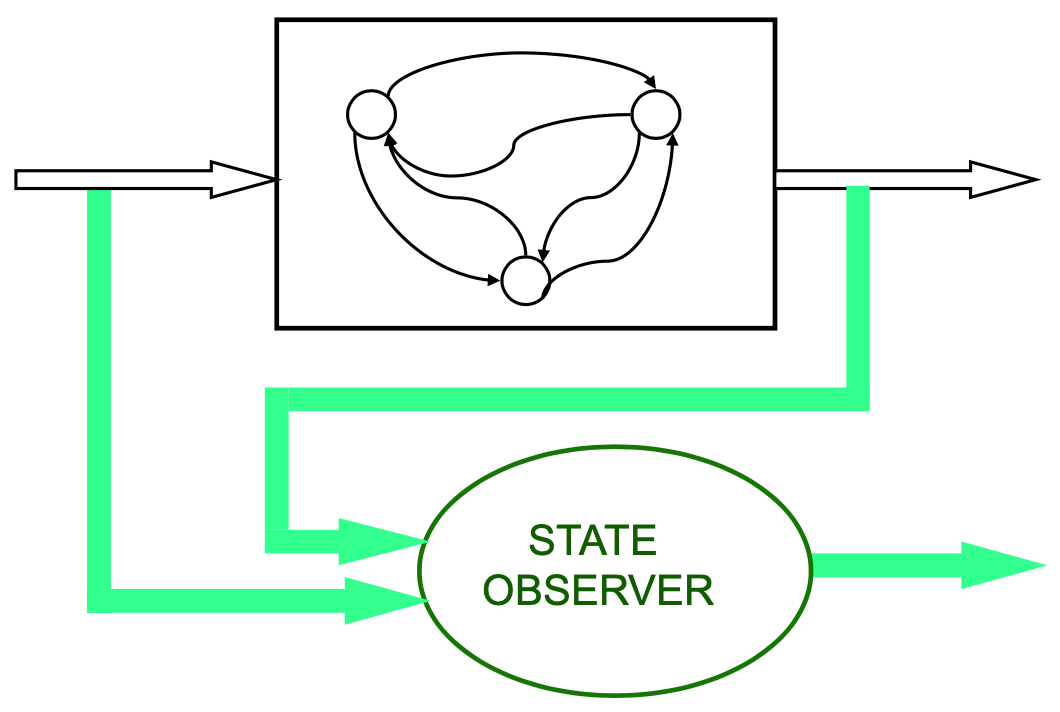
\includegraphics[scale=0.35]{immagini/obs}
	\caption{State observer}
	\label{fig:obs}
\end{figure}
We will firstly have a look to the problem of observer design for \emph{continuous time linear systems} and then transpose the concepts to \emph{switched linear systems} with switching signal available through measurements.
\subsection{Observer design for continuous time linear system}
The system we are dealing with is of the form:
$\begin{cases} 
	\dot{x}(t)=Ax(t)+Bu(t)\\
	y(t)=Cx(t)\\
\end{cases}$
where 
\begin{itemize}
	\item[] $u(t)\in \Re^m \equiv input$
	\item[] $y(t)\in \Re^p \equiv output$
	\item[] $x(t)\in \Re^n \equiv state$.
\end{itemize}
	\begin{figure}[H]
	\centering
	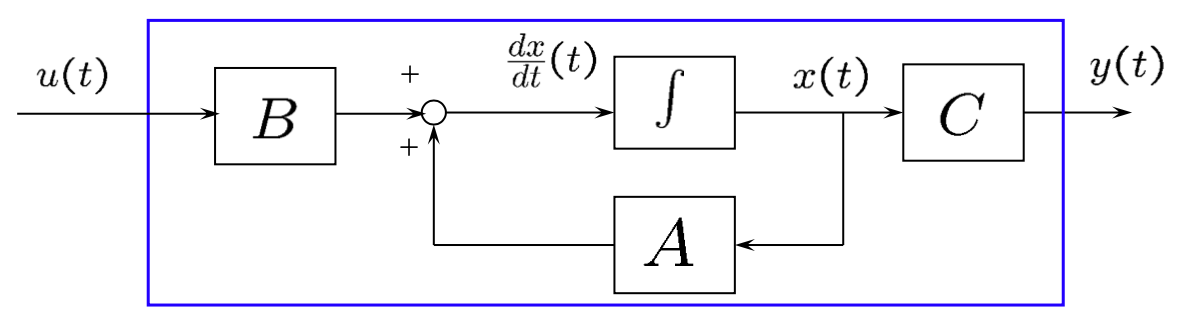
\includegraphics[scale=0.4]{immagini/cont-lin-sys}
	\caption{Continuous linear system}
	\label{fig:cont-lin-sys}
\end{figure}
\begin{defn}[Asymptotic or Lurenberger observer]
	An asymptotic observer is a system that consistently estimates the state x(t) based on the input and output measurements $u(\tau)$ and $y(\tau), 0 \le \tau \le t$, for any (unknown) initial condition $x_0$ and for any input $u(\cdot):$
	\[
	\lim_{t\rightarrow \infty}\|\hat{x}(t)-x(t)\|=0, \qquad \forall x(0)=x_0\in \Re^n, \forall u(\cdot)
	\]
\end{defn}
Essentially the observer is a copy of the original system with an extra exogenous input which depends on the output of the real system.
\begin{figure}[H]
	\centering
	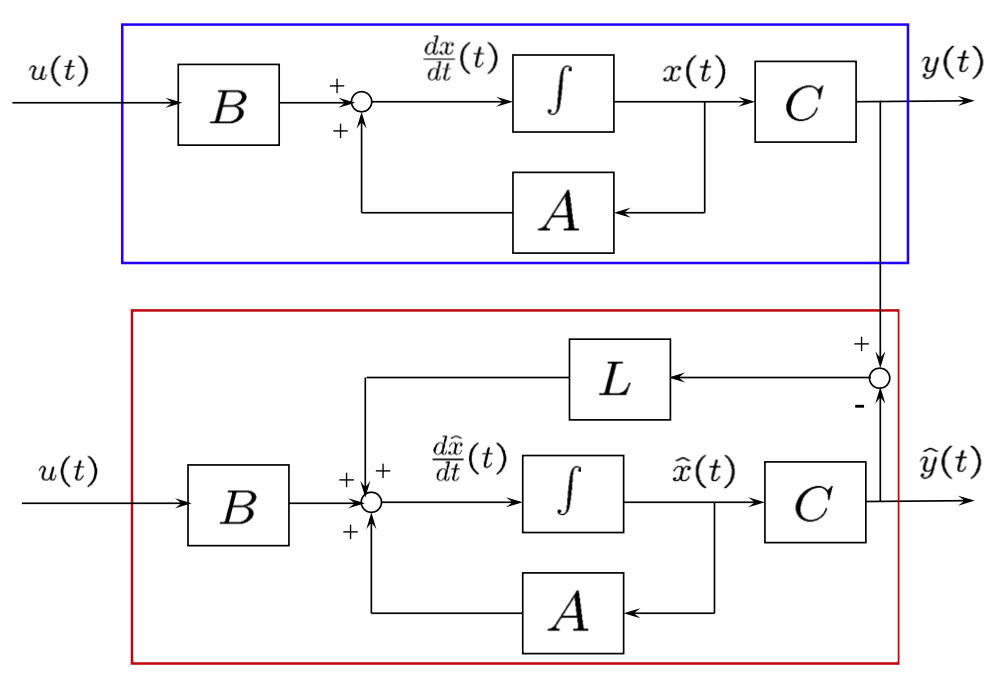
\includegraphics[scale=0.4]{immagini/observer}
	\caption[Asymptotic observer]{}
	\label{fig:observer}
\end{figure}
The equation of the observer is then:
\[
\begin{cases} 
	\dot{\hat{x}}(t)=A\hat{x}(t)+Bu(t)+\textcolor{red}{L}(y(t)-\hat{y}(t))\\
	\hat{y}(t)=C\hat{x}(t)\\
\end{cases}
\]
Defining the prediction state error $e(t)\colon= x(t)-\hat{x}(t)$ we complete the observer system result:
\[
\begin{cases} 
	\dot{\hat{x}}(t)=A\hat{x}(t)+Bu(t)+\textcolor{red}{L}(y(t)-\hat{y}(t))\\
	\hat{y}(t)=C\hat{x}(t)\\
	\dot{e}(t)=(A-LC)e(t)\\
\end{cases}
\]
If A is Hurwitz, then,
\begin{itemize}
	\item one can set L=0 and obtain that the estimation error converges exponentially to zero because when my system is asymptotically stable the contribution of the initial condition (which is unknown) goes to 0 so basically we don't need to reconstruct $x_0$;
	\item no output measurements are needed, but the rate of convergence will be determined by the real part of the eigenvalues of A.
\end{itemize}
But what if A is not asymptotically stable?
\begin{thm}
	If the couple (A,C) is detectable, then, L can be designed so that A-LC is Hurwitz and, hence, the estimation error converge exponentially to zero:
	\[
	\|e(t)\| \le \mu e^{-\lambda_0t}\|e(0)\|, t\ge 0, \qquad \forall e(0)=e_0 \in \Re^n
	\]
\end{thm}
In order to define the concept of detectability we need to define first the \textbf{observability} property:
\begin{defn}[Observable system]
	A system is observable if all states $x\neq0$ are observable that means that the observability matrix $O_n$ has maximum rank (n).
	\[
	O_n=\begin{bmatrix} 
		C \\
		CA\\
		CA^2\\
		\vdots\\ 
		CA^{n-1}
    \end{bmatrix}
	\]
\end{defn}
The key property is that if the couple (A,C) is observable one can select matrix L such that A-LC has arbitrarily chosen eigenvalues.

\begin{defn}
	A system is detectable if the eigenvalues of the unobservable parte have all striclty negative real part.\\
	In this case, the pair \textcolor{red}{(A,C)} is \textcolor{red}{detectable}.
\end{defn}
\subsubsection{Sketch of the proof}
Assume without loss of generality that the system is in the observable canonical form. If not, then we can use Kalman decomposition:  $w\colon=T_ox$
\begin{figure}[H]
	\centering
	\includegraphics[scale=0.4]{immagini/proof}
	\label{fig:proof}
\end{figure}
\[\begin{bmatrix}
	\dot{w}_o(t)\\
	\dot{w}_{no}(t)
\end{bmatrix}
=\begin{bmatrix}
	A_{11} & 0\\A_{21} & A_{22}
\end{bmatrix}\begin{bmatrix}
w_o(t)\\w_{no}(t)
\end{bmatrix}
+\begin{bmatrix}
	B_1\\B_2
\end{bmatrix}u(t)
\]
\[
y(t)=\begin{bmatrix}
	C_1 & 0
\end{bmatrix}\begin{bmatrix}
w_0(t)\\w_{no}(t)
\end{bmatrix}
\]
The dynamics of the estimation error is:
\[
\dot{e}(t)=\left(A-LC\right)e(t)\\
e_w\colon=T_oe
\]
and so
\[
\dot{e}_w(t)=\left( \begin{bmatrix}
	A_{11} & 0\\A_{21} & A_{22}
\end{bmatrix}-\begin{bmatrix}
	\tilde{L}_1 \\ \tilde{L}_2
\end{bmatrix} \begin{bmatrix}
C_1 & 0
\end{bmatrix}\right) e_w(t)=\begin{bmatrix}
	\boxed{A_{11}-\tilde{L}_1C_1} & 0\\
	A_{21}-\tilde{L}_2C_1 & \boxed{A_{22}}
\end{bmatrix} e_w(t)
\]
where $\tilde{L}=T_oL$.\\
The eigenvalues of $A_{11}-\tilde{L}_1C_1$ can be arbitrarily selected since $\left( A_{11},C_1\right)$ is observable and the eigenvalues of the unobservable part ($A_{22}$) are being keep fixed.
\begin{thm}
	If (A,C) is detectable, then, L can be designed so that A-LC is Hurwitz and, hence, the estimaton error converges exponentially to zero:
	\[
		\|e(t)\| \le \mu e^{-\lambda_0t}\|e(0)\|, t\ge 0, \qquad \forall e(0)=e_0 \in \Re^n
	\]
\end{thm}
\begin{remark}
	The convergence rate can be arbitrarily chosen if and only if (A,C) is observable.
\end{remark}
\subsection{Observer design for switched linear system}
Since we have a switching signal that at every time t dictate which system is active we have a kind of discrete system and two outputs.
\newline
Having the following kind of system:
\[
\dot{x}(t)=A_{\sigma(t)}x(t)+B_{\sigma(t)}u(t)\]
\[
y(t)=C_{\sigma(t)}x(t)
\]
and the switching occurs within the family of systems:
\[
\dot{x}(t)=A_qx(t)+B_qu(t) \]
\[
y(t)=C_qx(t)
\] with $ q=\left\{1,2,\dots,m\right\}$\\
\textcolor{red}{Assumptions:}
\begin{enumerate}
\item[(i)] the switching signal $\sigma\colon \left[0,\infty\right)\to Q$ is available as (discrete) output signal
\item[(ii)] $(A_q,C_q)$ is detectable for all $q\in Q$
\end{enumerate}
The idea here is the same as for linear system but we need to design an observer for each system that activate when the system is activated by the switching system.
\begin{figure}[H]
	\centering
	\includegraphics[scale=0.55]{immagini/s_ob}
	\caption{Switching observer}
	\label{s_on}
\end{figure}
As did before now we derive the dynamics of the estimation error from the system and observer equations:
\[\text{system}\colon \begin{cases}
	\dot{x}(t)=A_{\sigma(t)}x(t)+B_{\sigma(t)}u(t)\\
	y(t)=C_{\sigma(t)}x(t)
\end{cases}
\]
\[\text{observer}\colon \begin{cases}
	\dot{\hat{x}}(t)=A_{\sigma(t)}\hat{x}(t)+B_{\sigma(t)}u(t)+L_{\sigma(t)}(y)(t)-\hat{t}(t))\\
	y(t)=C_{\sigma(t)}x(t)
\end{cases}
\]
\[
\boxed{\dot{e}(t)=\left( A_{\sigma(t)}-L_{\sigma(t))}C_{\sigma(t)}\right)e(t)}
\]
\begin{thm}
	If there exists $P=P^T>0$ such that \[P(A_q-L_qC_q)+(A_q-L_qC_q)^TP<0, \forall q \in Q=\left\{1,2,\dots,m\right\}\] then, the switching observer consistently estimates the continuous state of the switched system, for any e(0) and for any $\sigma \colon \left[0,\infty\right) \to Q$.
\end{thm}

\begin{proof}
	 $V(e)=e^TPe$ is a radially unbounded common Lyapunov function at the equilibrium e=0. Then, e=0 is GUAS.
	\end{proof}
\paragraph{Switching observer design}
At this point we have to concretely design the observer and so its gains. The gains $L_1,L_2,\dots,L_m$ such that there exist $P=P^T>0$ satisfying: \[P(A_q-L_qC_q)+(A_q-L_qC_q)^TP<0, \forall q \in Q=\left\{1,2,\dots,m\right\}
\]
Since the product between P and $L_q$ makes the system non linear so we have to do a \textcolor{red}{Linear Matrix Inequalities (LMI) reformulation}.
By setting $L_q=P^{-1}Y_q$, we have $PL_q=Y_q$ the problem can then be rephrased as that of determining $P=P^T>0$ and $Y_1,Y_2,\dots,Y_m$ such that \[
PA_q-Y_qC_q+A_q^TP-C_q^TY_q^T<0, \forall q \in  Q =\left\{1,2,\dots,m\right\}
\]
Gains are then recovered by $L_q=P^{-1}Y_q$.
The implementation idea is to design the switching observer gains $L_1,L_2,\dots,L_m$ such that the dynamics of the estimation error $\dot{e}(t)=(A_{\sigma(t)}-L_{\sigma(t)}C_{\sigma(t)})e(t)$ is contractive over each switching time interval, and, hence $e(t)\to 0$, for any e(0) and for any $\sigma \colon \left[0,\infty\right)\to Q$ with minimum dwell time $\tau_D$.
\begin{remark}
	Stability under slow switching condition is forced by making the error dynamics fast compared with the given $\tau_D$.
\end{remark}
To do this in practice we have to relay on the \textbf{squashing lemma}:\\
Suppose (A,C) observable. Let $\tau_D>0$. Then, for any $\rho >0$ there exist $\alpha>0$ and L such that \[\|e^{(A-LC)t}\| \le \rho e^{-\alpha(t-\tau_D)}, t \ge 0\]
If one chooses $0<\rho<1$, then, the dynamics is contractive over each time interval of length larger than or equal to $\tau_D$. So it's crucial to know the length of the dwell time in order to design L. The system converges exponentially and if after a certain time the system doesn't switch anymore it is still stable and converging because is Hurwitz.
%%% Fine del capitolo%%%
	\pagebreak
	\chapter{Lur'e Problem}
\section{Definition of the Lur'e problem and staibility}
\begin{figure}[H]
	\centering
	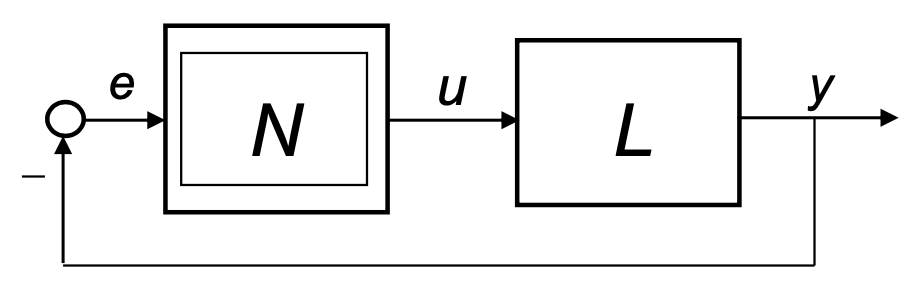
\includegraphics[scale=0.4]{immagini/lure1}
	\caption{Lur'e system}
	\label{fig:lure1}
\end{figure}
An autonomous Lur'e system is a feedback system with a nonlinear static component (N) in series with a linear component (L). The non linear part is defined with a function $\phi$ as follows: 
\[
N \colon u(t)=\phi(e(t)), \forall e 
\]with:
\begin{itemize}
		\item $\phi \colon \Re \to \Re$
		\item $\phi(\cdot) \in \Phi_{\left[k_1,k_2\right]}$.
\end{itemize}
While the linear part is simply:
\[
L:  \begin{cases}
	\dot{x}=Ax+Bu \\ y=Cx
\end{cases}
\] with the assumption of (A,B) reachable and (A,C) observable.
\\ The $\phi$ function is meant to be continuous and to belong to a \textbf{sector nonlinearity}.
\begin{figure}[H]
	\centering
	\includegraphics[scale=0.4]{immagini/snl}
	\caption{Sector nonlinearity}
	\label{fig:snl}
\end{figure}
The sector is plotted in the e-u space taking e as an input and u as the output and it's defined by two lines of slope $k_1$and $k_2$. The sector of nonlinearity is the sector that contains all the $\phi$ funcitons which satisfy the following condition:
\[
\Phi_{\left[k_1,k_2\right]}=\left\{\phi(\cdot)\colon (k_2e-u)(u-k_1e)\ge 0, u=\phi(e), \forall e \in \Re\right\}
\]
Since the sector enforce the function to pass from 0 in any case and: $f(x)\colon=Ax+B\phi(-Cx)$ if $\phi(0)\to 0$ also $f(0)\to 0$ and so $\bar{x}=0$ is an equilibrium for S, for any section nonlinearity $\phi(\cdot) \in \Phi_{\left[k_1,k_2\right]}$.
\subsubsection{Absolute stability in the sector $[k_1,k_2]$}
\begin{defn}
	System \textcolor{red}{S} is \textcolor{red}{absolutely stable in the sector $[k_1,k_2]$} if x=0 is a globally asymptotically stable (GAS equilibrium, for every sector non linearity) $\phi(\cdot) \in \Phi_{\left[k_1,k_2\right]}$.
\end{defn}
So the Lur'e problem, given the transfer function G(s) of the linear system L, \textcolor{red}{determine necessary and/or sufficient conditions for the absolute stability} of S in the sector $[k_1,k_2]$.
\subsection{Necessary condition for absolute stability} \label{S_L}
\begin{figure}[H]
	\centering
	\includegraphics[scale=0.4]{immagini/snl2}
	\caption{$\phi(\cdot) \in \Phi_{[k_1,k_2]}$}
	\label{fig:snl2}
\end{figure}
Since $\phi$ is a general static function in a sector, among all the nonlinear set of functions we have for sure also the linear ones, so if we want to get absolute stability in the sector we have to consider all the possible functions, including the linear ones. It's \textbf{necessary} that when we restrict the set of funcitons to the linear ones to have asymptotical stability, but it's not sufficient.
\begin{figure}[H]
	\centering
	\includegraphics[scale=0.4]{immagini/sl}
	\caption{$\phi(e)= ke  \in \Phi_{[k_1,k_2]}$}
	\label{fig:sl}
\end{figure}
If S is absolutely stable in $[k_1,k_2]$, then , $S_L$ is (globally) asymptotically stable for any $k \in [k_1,k_2]$. If $0 \in [k_1,k_2]$, then, system L with transfer function G(s) is asymptotically stable.\\
So if we have a \underline{given k}, system $S_L$ is asymptotically stable if and only if the Nyquist plot of G(s) encircles (anti-clockwise) the point in the complex plan corresponding to the real number $-\frac{1}{k}$ as many times as the number of poles of G(s) with positive real part (\emph{Nyquist criterion})
\begin{figure}[H]
	\centering
	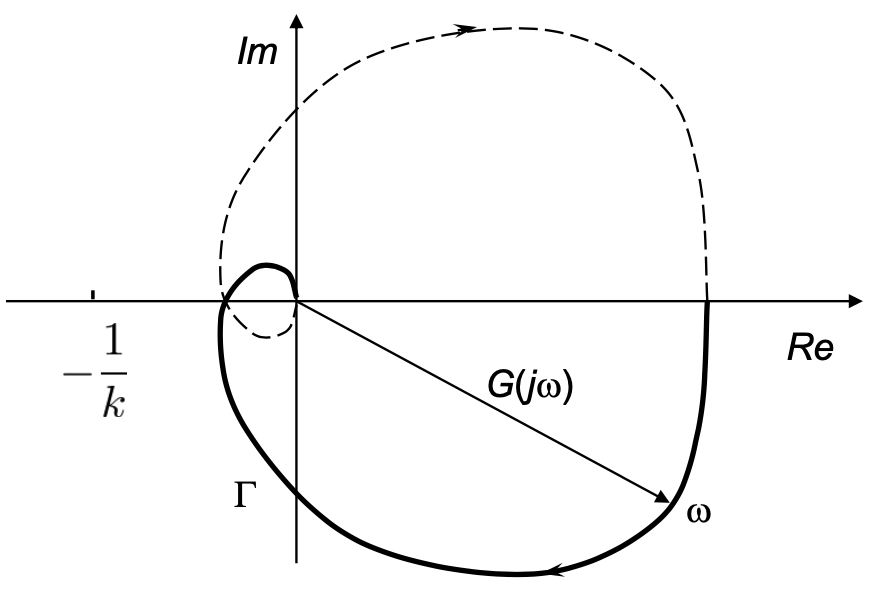
\includegraphics[scale=0.4]{immagini/nyq}
	\caption{Nyquist criterion}
	\label{fig:nyq}
\end{figure}
Now let's move a step further. Actually "k" can ranging in the sector $[k_1,k_2]$ so we can adapt the previous statement changing the value $-\frac{1}{k}$ with an interval defined as follows: \[I(k_1,k_2)\colon= \left\{\alpha \in \Re\colon \alpha =-\frac{1}{k}, k \in [k_1,k_2]\right\}\]
\begin{figure}[H]
	\centering
	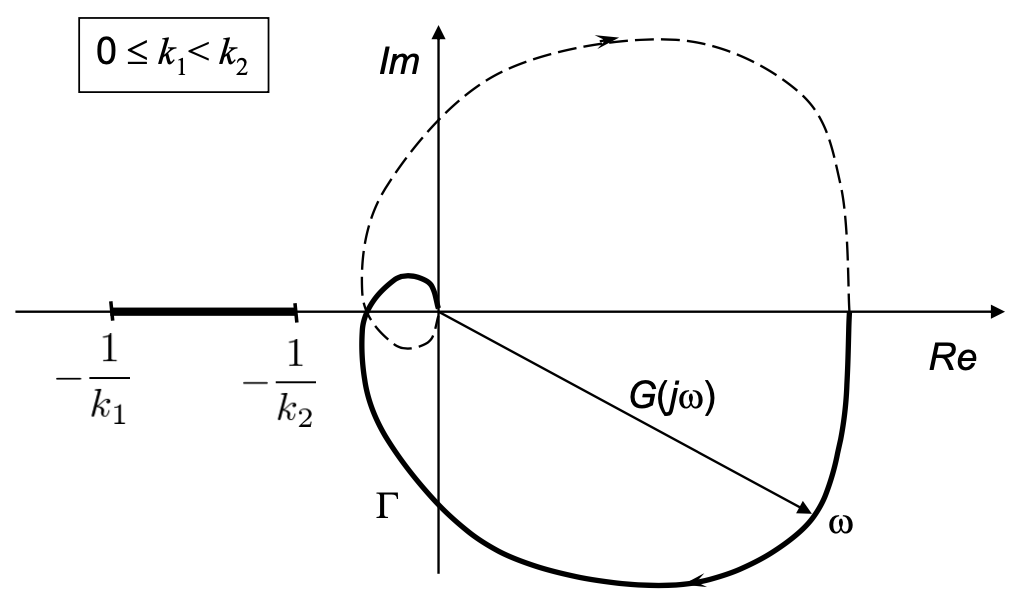
\includegraphics[scale=0.4]{immagini/nyq2}
	\caption{Nyquist criterion with an interval}
	\label{fig:nyq2}
\end{figure}
So for an \underline{uncertain k}, system $S_L$ is asymptotically stable for any $k\in[k_1, k_2]$ if and only if the Nyquist plot of G(s) encircles (anti-clockwise) $I(k_1,k_2)$ as many times as the number of poles of G(s) with positive real part.
\\ We can now state the theorem:
\begin{thm}[Necessary condition for absolute stability of an autonomous Lur'e system]
	If S is absolutely stable in the sector $[k_1, k_2]$, then the Nyquist plot of G(s) encircles (anti-clockwise) $I(k_1,k_2)$ as many times as the number of poles of G(s) with positive real part.
	In particular, if $0\in[k_1, k_2]$, then system L with transfer function G(s) is asymptotically stable.
\end{thm}
To sum up in Figure \ref{fig:nyqtot} are represented all the possible cases of sector configurations.
\begin{figure}[H]
	\centering
	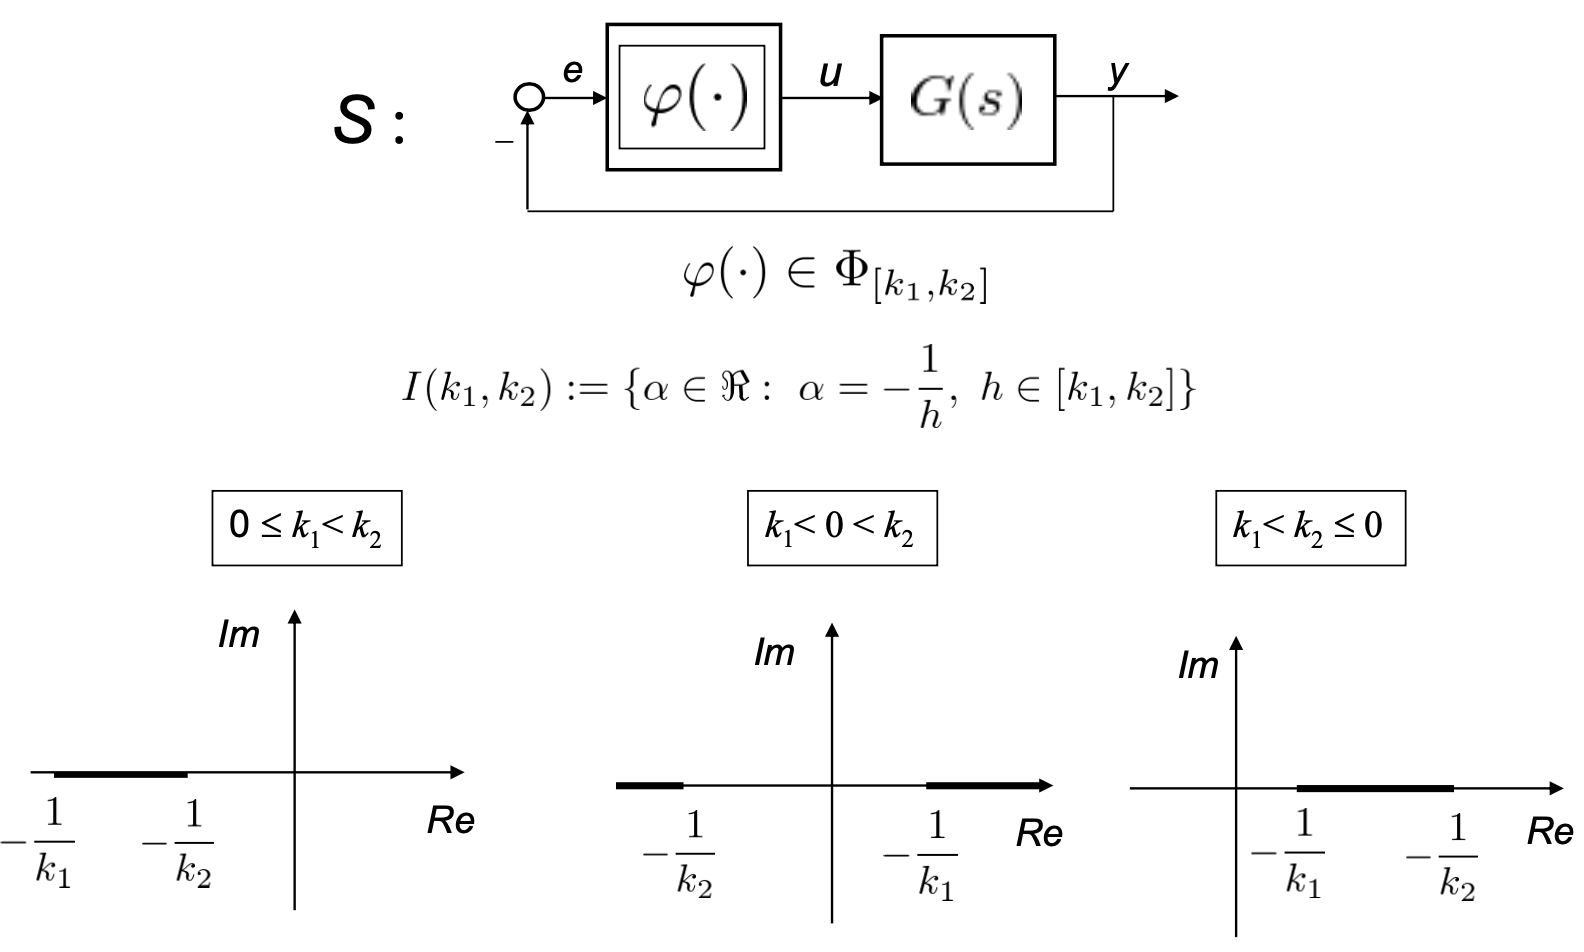
\includegraphics[scale=0.4]{immagini/nyqtot}
	\caption{Impact of the sector boundaries on Nyquist plot}
	\label{fig:nyqtot}
\end{figure}
 Notice that if one of the two ''k''s is equal to 0, one boundary of the interval \emph{I} diverges to infinity and so the Nyquist plot with the interval result as in Figure \ref{fig:nyq0}. So in practice in this case the Nyquist plot should not cross the semi line in question.
\begin{figure}[H]
 	\centering
 	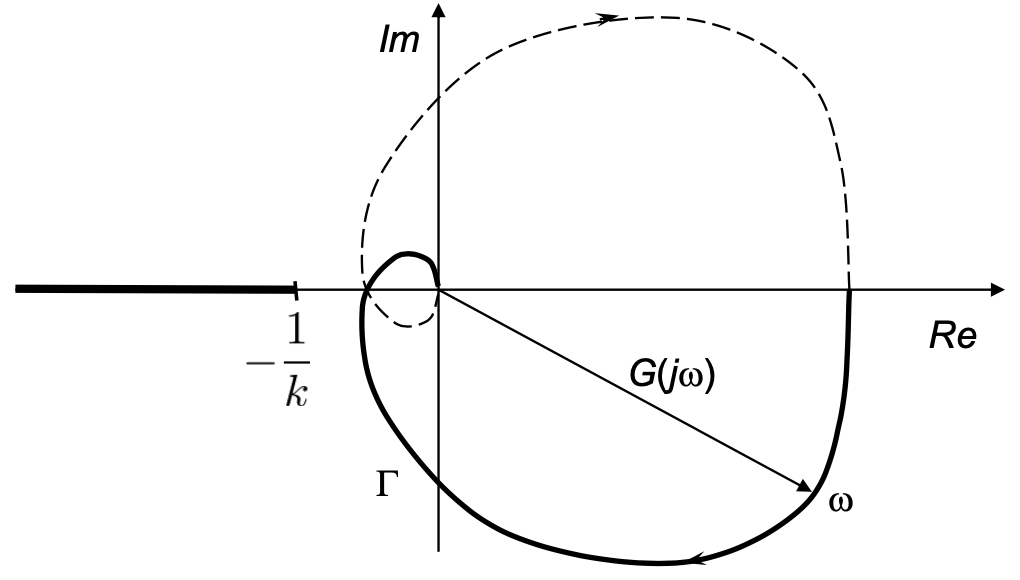
\includegraphics[scale=0.4]{immagini/nyq0}
 	\caption{$[0,k]$ sector}
 	\label{fig:nyq0}
\end{figure}
\subsection{Conjectures}
\subsubsection{Aizerman conjecture (1949):}
The necessary condition is also sufficient.
\subsubsection{Kalman conjecture (1960):}
If $\phi(\cdot)$ is differentiable with continuous derivative and it holds that 
\[
k_1\le\frac{d\phi}{de}(e)\le k_2, \qquad \forall e\in\Re
\]then the necessary condition is also sufficient.\\
But this conjectures are proven to be false with some non-trivial counterexamples we will omit. The fundamental message here is that the solution to Lur'e problem cannot be rephrased in terms of linear system analysis.
\linebreak
So now we want to study some sufficient and practical condition but not sufficient: the Popov and circle criteria.
\section{Popov Criterion}
\begin{thm}[sufficient condition for the absolute stability of S in sector \textcolor{red}{[0,k]}, Popov criterion, 1962] 
	System S is absolutely stable in sector [0,k] if system L is asymptotically stable (necessary condition), and if there exists a real number ''q'' such that the following condition is satisfied: 
	\[
	\Re\left[(1+j\omega q)G(j\omega\right)] > -\frac{1}{k}, \forall \omega \ge 0
	\]
\end{thm}
In order to better understand and use this theorem is very useful to have a sight at its graphical interpretation. 
\subsection{Graphical interpretation of Popov criterion}
We will work with a given transfer function G(s).\\  The first step is to draw the polar plot of G(s) setting \boxed{q=0} and check if it is entirely located on the right-hand-side of the straight line passing through $-\frac{1}{k}$ and parallel to the imaginary axis. In this way the necessary condition for absolute stability is satisfied.
\begin{figure}[H]
	\centering
	\includegraphics[scale=0.3]{immagini/popovq0} \qquad
	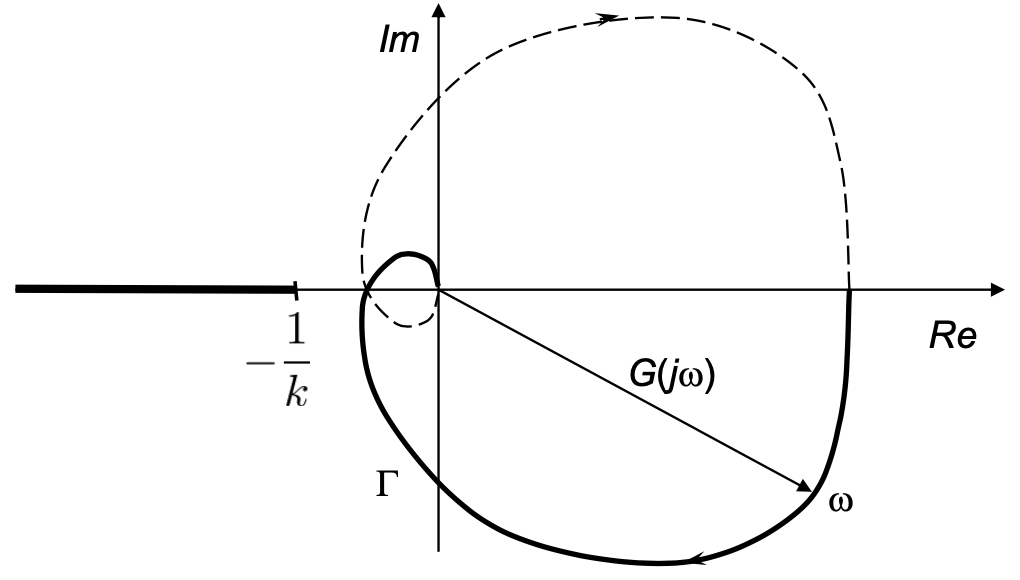
\includegraphics[scale=0.3]{immagini/nyq0}
	\label{fig:popovq0}
\end{figure}
Let's now remove the assumption of having q=0 and draw the polar plot $\Gamma^*$ of G*(s) with a \boxed{q\ne0}. We call this the Popov plot and essentially is a rescaled polar plot along the imaginary axis by $\omega$. For this reason the Popov plot and the polar plot shares the same points on the real axis.
\[
G^*(j\omega)=\operatorname{Re}[G(j\omega)]+j\omega\operatorname{Im}[G(j\omega)]
\]
\begin{figure}[H]
	\centering
	\includegraphics[scale=0.4]{immagini/popovplot}
	\caption{Popov plot}
	\label{fig:popovplot}
\end{figure}
We now have to find out if there exist a straight line passing through $-\frac{1}{k}$ (\emph{Popov line}) such that $\Gamma^*$ is on the open half plane on its right-hand-side. But how can we identify that line? Let's do a bit of computation.
\[
G^*(j\omega)=\operatorname{Re}[G(j\omega)]+j\omega\operatorname{Im}[G(j\omega)]
\]
\[ \operatorname{Re}[(1+j\omega q)G(j\omega)]=\operatorname{Re}[G(j\omega)]-q\operatorname{Im}[G(j\omega)]=a^*-qb^*\] where $a^*\colon=\operatorname{Re}[G^*(j\omega)]$ and $b^*\colon=\operatorname{Im}[G^*(j\omega)]$.
So applying the Popov criterion condition: \[\operatorname{Re}[(1+j\omega q)G(j\omega)]=a^*-qb^*>-\frac{1}{k},\forall\omega \ge0\] we will have to different resulting lines depending on the sign of q.
\[
b^*<\frac{1}{q}(a^*+\frac{1}{k}), \text{if} q >0 \qquad \qquad b^*>\frac{1}{q}(a^*+\frac{1}{k}), \text{if} q <0 
\]
\begin{figure}[H]
	\centering
	\includegraphics[scale=0.35]{immagini/popovlineslope}
	\caption{Popov lines}
	\label{fig:popovlineslope}
\end{figure}
So in the end we have that the slope if this curve is $\frac{1}{q}$.
\subsection{Aizerman conjecture}
For this particular case, having a sector of the shape $[0,k]$, and so the Popov criterion holds, we want to check if the Aizerman conjecture is satisfied for a particular G(s). We will proceed as follows:
Given G(s), let us denote:
\begin{itemize}
	\item $K_P$ (P refers to Popov and it is $>0$) the largest value such that the absolute stability of S in the sector [0,h] is guaranteed via Popov criterion for any $h\in[0,K_P)$
	\item $K_N$ the largest K such that the linear system $S_L$ is asymptotically stable fo any $h\in[0,K_N)$
\end{itemize}
Evidentely $K_P\le K_N$ because we can't have absolute stability and not asymptotic stability a linear system associated to our autonomous system. Thus in the case $K_P=K_N$ the system satisfies Aizerman conjecture, while if $K_P<K_N$ no conclusion can be drawn since Popov criterion is a sufficient condition for the absolute stability of S.
\linebreak
Let's now do some example in order to clarify this concept and the relation between Popov plot and sector nonlinearity.

\paragraph{Example}	Given the following transfer function \textbf{$G(s)=\frac{80}{(1+0.5s)^3}$} we have to compute a maximum sector over which absolute stability is hold and compare it with the maximum range of variability for K to replace in the nonlinear block such that the ''linearized'' system satisfies asymptotic stability.
\begin{figure}[H]
	\centering
	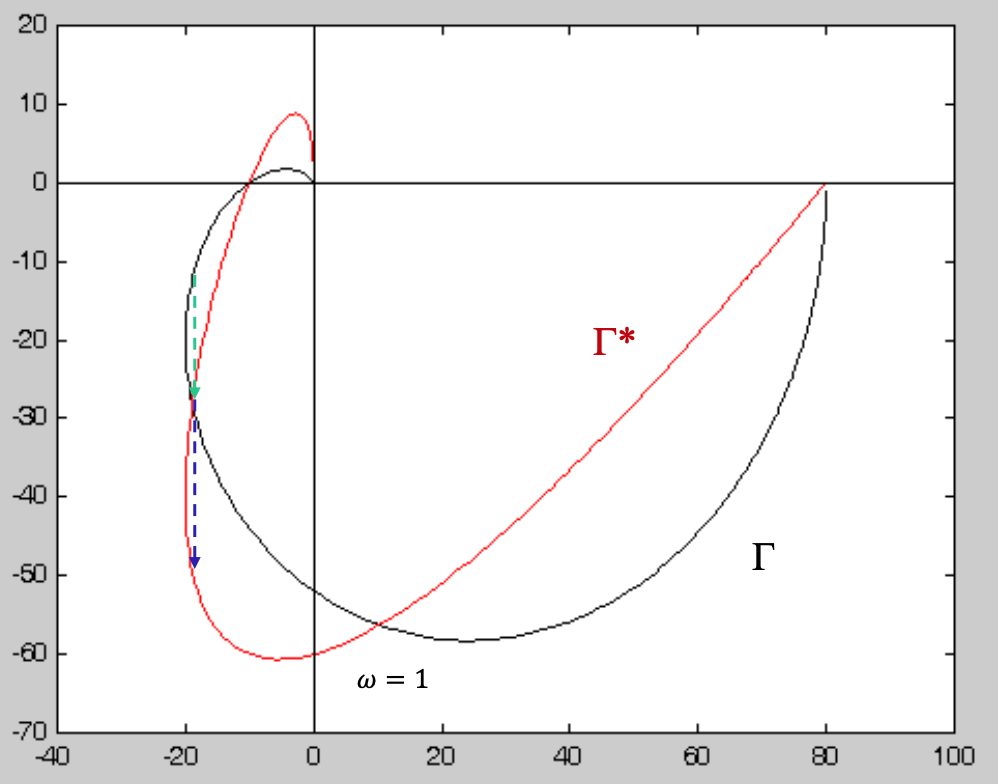
\includegraphics[scale=0.4]{immagini/ex1}
	\caption{Comparison between Popov plot and polar plot of G(s)}
	\label{fig:ex5}
\end{figure}
We know want to identify on the plot $K_N$ and $K_P$.
\begin{figure}[H]
	\centering
	\begin{subfigure}[b]{0.3\textwidth}
		\centering
		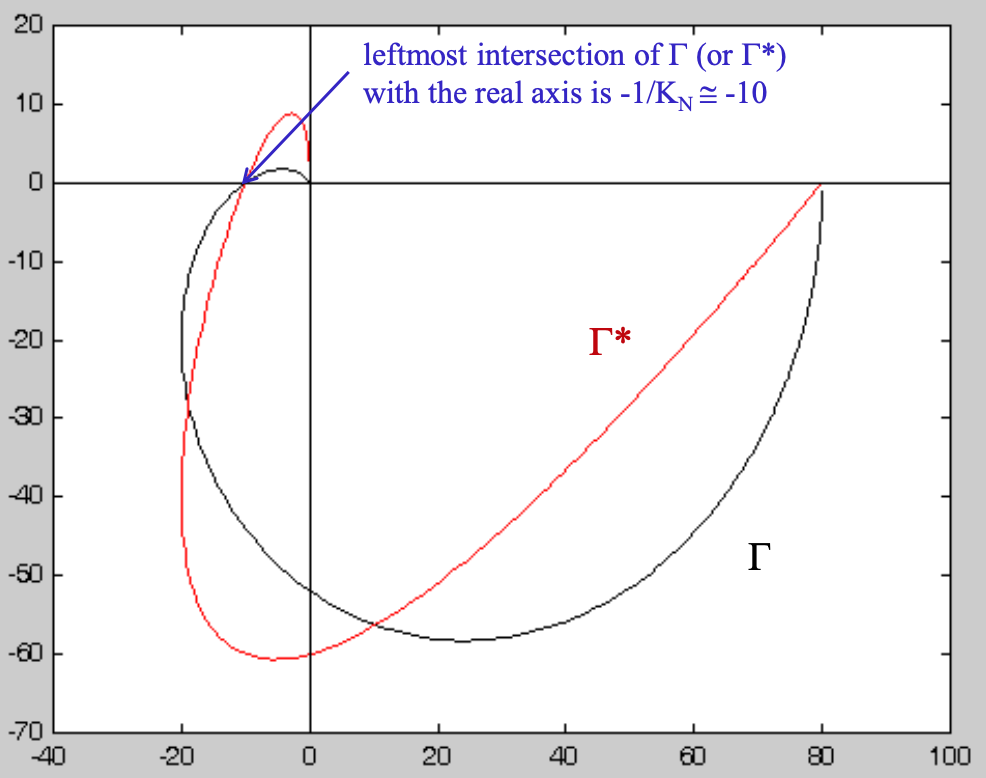
\includegraphics[scale=0.25]{immagini/ex2}
		\caption{$K_N$}
		\label{fig:kn}
	\end{subfigure}
	\hfill
	\begin{subfigure}[b]{0.3\textwidth}
		\centering
		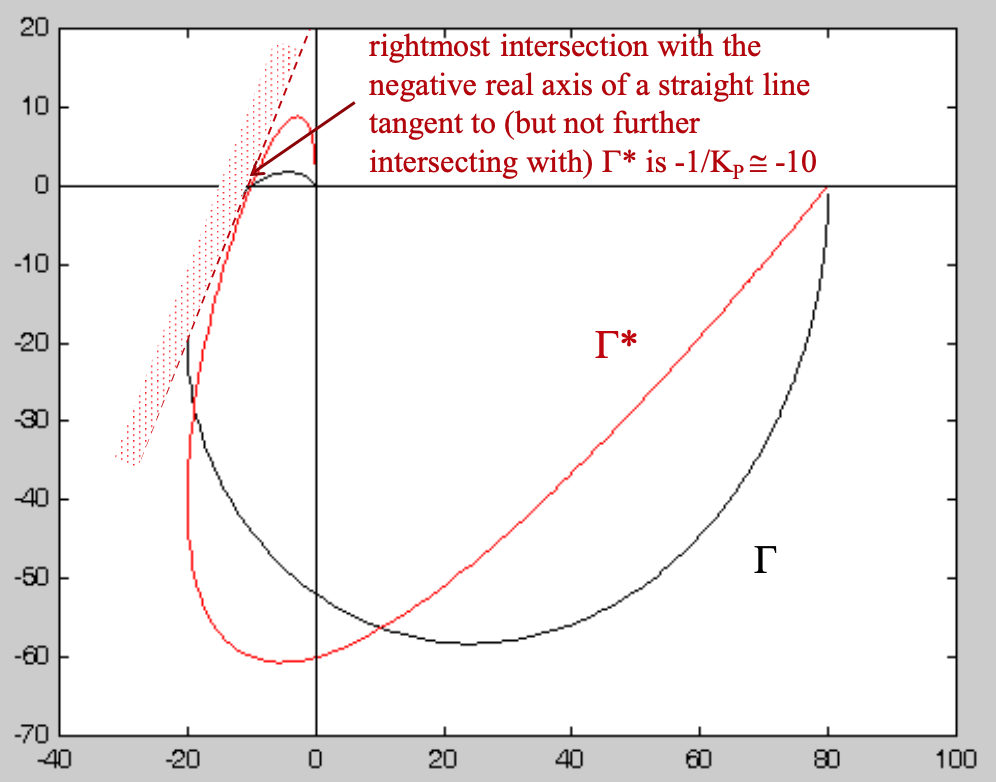
\includegraphics[scale=0.25]{immagini/ex3}
		\caption{$K_P$}
		\label{fig:kp}
	\end{subfigure}
	\hfill
	\label{fig:esempio1}
\end{figure}
In this example $K_P=K_N\cong 0.1$ and, hence, S is absolutely stable in the sector [0,h], for any $h \in [0,0.1)$ and $S_L$ is asymptotically stable for any $h \in [0,0.1)$. $\Longrightarrow$ \textbf{Aizerman conjecture is satisfied}.

\paragraph{Example} Now we will do the same procedure but with a different general transfer function with 3 zeros and 4 poles.\[G(s)=\frac{\mu(1+sT_1)(1+sT_2)^2}{(1+sT_3)^2(1+sT_4)(1+sT_5)}\]
\begin{figure}[H]
	\centering
	\begin{subfigure}[b]{0.3\textwidth}
		\centering
		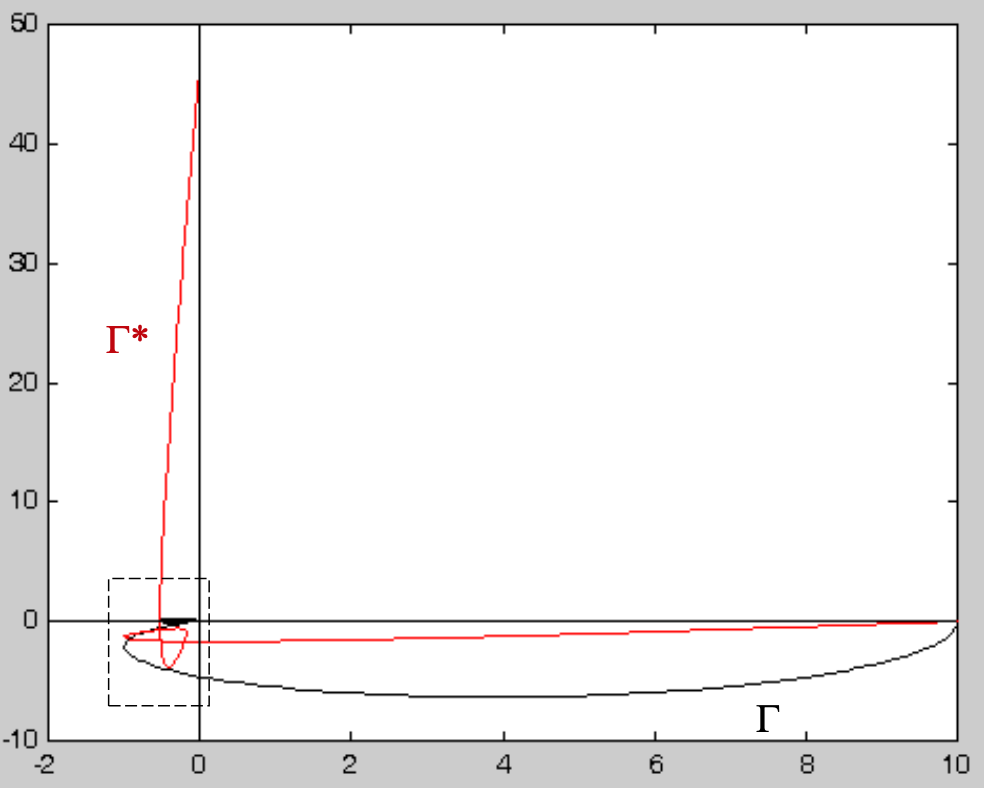
\includegraphics[scale=0.25]{immagini/ex4}
		\caption{$K_P<K_N$ transfer function}
		\label{fig:plopov}
	\end{subfigure}
	\hfill
	\begin{subfigure}[b]{0.3\textwidth}
		\centering
		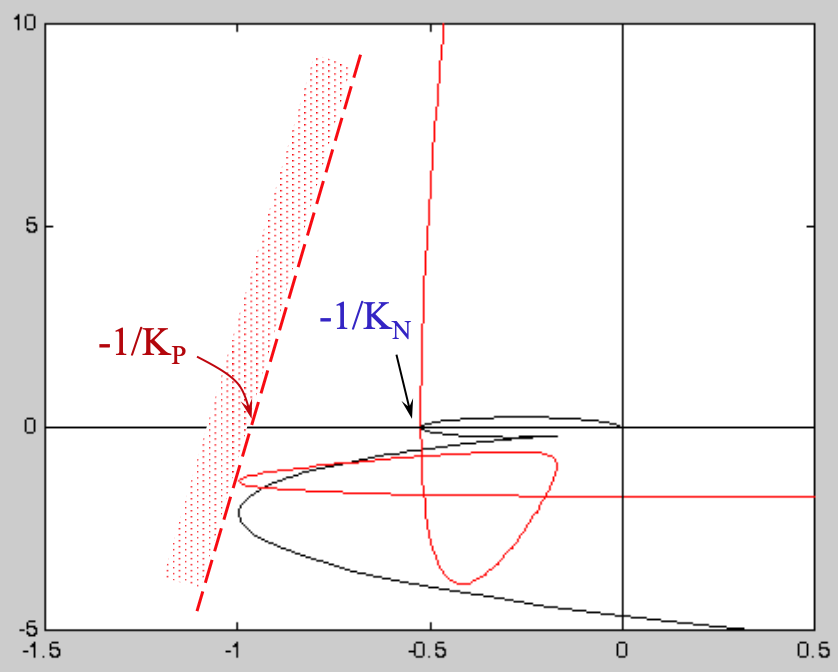
\includegraphics[scale=0.3]{immagini/ex5}
		\caption{$K_N$ and $K_P$ identification}
		\label{fig:kp&kn}
	\end{subfigure}
	\hfill
	\label{fig:esempio2}
\end{figure}
In this example $K_P\cong1.1<K_N\cong1.8$, and, hence, S is absolutely stable in the sector [0,h], for any $h\in[ 0,1.1)$ while $S_L$ is asymptotically stable for any $h\in[0,1.8)$. So, is Aizerman conjecture satisfied? $\Rightarrow$ Maybe ...
\section{Circle criterion}
In this section we will treat the second sufficient condition for absolute condition, the circle criterion, and how is related to the Popov criterion and why can be seen as a corollary of the latter.\\
Since the Popov criterion holds only for nonlinear sector of the shape $[0,k]$ we need to extend the nonlinearity in the sector $[k_1,k_2]$. The trick is to transform the system with nonlinearity in  $[k_1,k_2]$  in another equivalent system but with a sector nonlinearity as the previously aimed $[0,k]$.
\begin{figure}[H]
	\centering
	\includegraphics[scale=0.5]{immagini/extensions}
	\caption{Extension to nonlinearity in sector $[k_1,k_2]$}
	\label{fig:extensions}
\end{figure}
\[
\left.
\begin{aligned}
	& \eta(e)=\phi(e)-k_1e, e\in Re	\\
	& k_1e\le \phi(e)\le k_2e,e \in \Re
\end{aligned}
\right\rbrace
\to \eta(\cdot)\in \Phi_{[0,k_2-k_1]}
\]while $F(s)=\frac{G(s)}{1+k_1G(s)}$.\\
From the equivalence between the two systems we have that system S is absolutely stable in the sector $[k_1,k_2]$ if and only if the system $S_0$ is absolutely stable in sector [0,k] with $k=k_2-k_1$.
\begin{note}
	The circle criterion is a restriction of Popov criterion because it requires q=0.
\end{note}
So if q=0, then, we have to check the following conditions:
\begin{enumerate}
	\item F(s) is the transfer function of an asymptotically stable system;
	\item $\Re[F(j\omega)]>-\frac{1}{k}, \forall \omega \ge0$ with $k=k_2-K_1$
\end{enumerate}
\paragraph{Condition 1} G(s) has to satisfy the necessary condition for the absolute stability of S in the sector $[k_1,k_2]$, that is the Nyquist plot of G(s) has to encircle anticlockwise $I(k_1,k_2)$, and hence the point $-\frac{1}{k}$, as many times as the number of poles of G(s) with positive real part. This leads to the result that F(s) is the transfer function of an asymptotically stable system by Nyquist criterion.
\paragraph{Condition 2} We shall rephrase the condition $\Re[F(j\omega)]>-\frac{1}{k}, \forall \omega \ge0$ in an suitable one on the polar plot of $G(j\omega)$.\\
We can map the polar plot of G(s) in function of F(s): $G(s)=F(s)(1+k_1G(s))\to G(s)(1-k_1F(s))=F(s)\to G(s)=\frac{F(s)}{1-k_1F(s)}$. So mapping every point s of F(s) through the transformation $\tilde{s}=\frac{s}{1-k_1s}$ we can draw the polar plot of G(s). And of course also the boundary region has to be transformed and the result will be the circle of the circle criterion that should not be intersected by the polar plot.
\begin{figure}[H]
	\centering
	\includegraphics[scale=0.4]{immagini/cond2}
	\caption{Rephrasing of the second condition in a suitable one the polar plot of $G(j\omega)$}
	\label{fig:cond2}
\end{figure}
\begin{note}
	It's not surprising that the left-hand side of the  line is mapped in the inside of the circle because if you take the intersection of the circle with the real axis we get an interval $I(k_1,k_2)$ of the Nyquist criterion, which is a necessary condition to be satisfied by $G(j\omega)$. Since Nyquist criterion is a necessary condition, the plot of $G(j\omega)$ should encircles the interval a number of times equals to the number of pole of $G(j\omega)$ with positive real part. 
\end{note}
Finally we can state a theorem.
\begin{thm}[sufficient condition for the absolute stability of S in the sector \textcolor{red}{$[k_1,k_2]$}, Circle criterion]
	System S is absolutely stable in the sector $[k_1,k_2]$, if the Nyquist plot of G(s) encircles (anti-clockwise) the circle $O(k_1, k_2)$ as many times as the number of poles of G(s) with positive real part.
\end{thm}
\begin{note}
	Since the Circle criterion is a corollary of Popov criterion, if the first fails we can go back to Popov and try with a $q\neq 0$.
\end{note}
\begin{figure}[H]
	\centering
	\includegraphics[scale=0.4]{immagini/circpopv}
	\caption{Relation between segments and circle in Circle and Nyquist criterion}
	\label{fig:circpopv}
\end{figure}
\section{Time varying Lur'e systems}
In this section we will analyze again the Lur'e system but this time the nonlinearity is also time varying.\begin{figure}[H]
	\centering
	\includegraphics[scale=0.4]{immagini/tvarlur}
	\caption{Time varying non linearity in  Lur'e system}
	\label{fig:tvarlur}
\end{figure}
Given the assumption of reachability of the couple (A,B) and observability of the couple (A,C) the non linear part is defined as follows:
\[
N \colon u(t)=\phi(e(t)), \forall e 
\]
While the linear part is simply:
\[
L:  \begin{cases}
	\dot{x}=Ax+Bu \\ y=Cx
\end{cases}
\] 
\\As before, The $\phi$ function is ment to be continuous and to belong to a \textbf{sector nonlinearity}.
\begin{figure}[H]
	\centering
	\includegraphics[scale=0.4]{immagini/tvarsec}
	\caption{Nonlinearity for a given $\bar{t}$, the sector remains the same, the curve change.}
	\label{fig:tvarsec}
\end{figure}
The sector is plotted in the e-u space taking e as an input and u as the output and it's defined by two lines of slope $k_1$and $k_2$. The sector of nonlinearity is the sector that contains all the $\phi$ funcitons which satisfy the following condition:
\[
\phi(\cdot,t) \in \Phi_{[k_1,k_2]}=\left\{\phi(\cdot)\colon k_1e^2\le\phi(e)e\le k_2e^2, \forall e \in \Re  \right\} \forall t \in \Re.
\]
Since the sector enforce the function to pass from 0 in any case and: $f(x(t),t)\colon=Ax(t)+B\phi(-Cx(t),t)$ if $\phi(0,\cdot)\to 0$ also $f(0,\cdot)\to 0$ and so $\bar{x}=0$ is an equilibrium for S, for any section nonlinearity $\phi(\cdot,t) \in \Phi_{\left[k_1,k_2\right]}$.

\subsubsection{Absolute stability in the sector $[k_1,k_2]$}
\begin{defn}
	System \textcolor{red}{S} is \textcolor{red}{absolutely stable in the sector $[k_1,k_2]$} if x=0 is a globally \textbf{uniformly} asymptotically stable (GUAS) equilibrium for all nonlinearities in the given sector.
\end{defn}
But now we have to formally explain what is meant with the notion of "uniform" stability.
\subsection{Uniform stability notions}
Given a dynamic system:
\[\dot{x}(t)=f(x(t),t)\] suppose that $f(o,\cdot)=0$. The equilibrium x=0 is:
\begin{itemize}
	\item stable if \[\forall\epsilon>0 \exists \gamma(\epsilon,t_0)>0\colon\|x(t_0)\|>\gamma\to\|x(t)\|<\epsilon,\forall t\ge t_0\]
	\item asymptotically stable if it is stable and \[\exists c(t_0)>0\colon \lim_{t\rightarrow \infty}x(t)=0,\forall\|x(t_0)\|)<c(t_0)	\]
	\item uniformly stable if \[\forall\epsilon>0 \exists \gamma(\epsilon)>0\colon\|x(t_0)\|>\gamma\to\|x(t)\|<\epsilon,\forall t\ge t_0\]
	\item uniformly asymptotically stable if it is uniformly stable and \[ \exists c >0\colon \lim_{t\rightarrow\infty}x(t)=0,\forall \|x(t_0)\|<c\] with convergence to zero that is uniform in $t_0$, i.e \[\forall\epsilon>0\exists T(\epsilon)>0\colon\|x(t)\|<\epsilon\forall t\ge t_0+T(\epsilon),\forall \|x(t_0)\|<c\]
	\item globally uniformly asymptotically stable if it is uniformly stable and \[\forall \epsilon >0 \text{ and } c>0 \exists T(\epsilon,c)> 0\colon\|x(t)\|<\epsilon, \forall t \ge t_0+T(\epsilon,c), \forall\|x(t_0)\|<c\]
\end{itemize}
\subsection{Lyapunov theorem for time varying system} \label{LYAptv}
Let's recall Lyapunov stability theorem for time varying system of the form:\[\dot{x}(t)=f(x(t),t)	\]
Let x=0 be an equilibrium\\If $V\colon [0,\infty]\times 	Re^n\to\Re$ is a $C^1$ function such that:\[W_1(x)\ge V(t,x) \ge W_2(x)\]\[\frac{\delta V}{\delta t}+\frac{\delta V}{\delta x}f(x,t)\le-W_3\] where $W_1(x), W_2(x), W_3(x)$ are continuous and positive definite funcitons, then, x=0 is uniformly asymptotically stable.\\Furthermore, if $W_1(x)$ is radially unbounded, then x=0 is \textbf{globally} uniformly asymptotically stable.\\Consider\[V(t,x)=x'Px,P=P'>0\] as candidate Lyapunov function. Then, one only needs to show that \[\dot{V}(t,x)=f(x,t)'Px+x'Pf(x,t)\le-W_3(x),\forall t\ge 0,\forall x \in \Re^n\] with $W_3(x)$ positive definite.
\begin{proof}
	\[W_1(x)=\lambda_{min(P)}\|x\|^2\le x'Px\le\lambda_{max}(P)\|x\|^2=W_2(x)\] $W_2(x), W_3(x)$ positive definite and $W_1(x)$ radially unbounded
\end{proof}
With this preliminary consideration we are now able to find a sufficient condition for the absolute stability.
\subsection{Necessary condition}
\begin{thm}[Necessary condition for absolute stability of a time invariant Lur'e system]
	If S is absolutely stable in the sector $[k_1, k_2]$, then the Nyquist plot of G(s) encircles (anti-clockwise) $I(k_1,k_2)$ as many times as the number of poles of G(s) with positive real part.
	In particular, if $0\in[k_1, k_2]$, then system L with transfer function G(s) is asymptotically stable.
\end{thm}
\begin{note}
	This theorem is exactly the same as for time invariant Lur'e systems because it is a robust version of Nyquist theorem and we can see the time invariant system as a particular case of the more general time varying. So if it holds for a particularity has to be necessary also for the general case.
\end{note}
\subsection{Popov criterion}
We are not proving it but Popov criterion also holds for time varying case but \textbf{only with q=0}, which is the main difference between time varying and invariant Lur'e systems.
\begin{thm}[sufficient condition for the absolute stability of S in sector \textcolor{red}{[0,k]}, Popov criterion, 1962] 
	System S is absolutely stable in sector [0,k] if system L is asymptotically stable (necessary condition), and if Popov condition is satisfied with q=0.
	\[
	\Re\left[G(j\omega)\right] > -\frac{1}{k}, \forall \omega \ge 0
	\]
\end{thm} And not surprisingly since Popov criterion holds for q=0 we can derive the corollary which is Circle criterion.
\subsection{Circle criterion}
\begin{thm}[sufficient condition for the absolute stability of S in the sector \textcolor{red}{$[k_1,k_2]$}, Circle criterion]
	System S is absolutely stable in the sector $[k_1,k_2]$, if the Nyquist plot of G(s) encircles (anti-clockwise) the circle $O(k_1, k_2)$ as many times as the number of poles of G(s) with positive real part.
\end{thm}
Circle criterion (as we can see the statement it has the same formulation), holds true also for time varying systems but absolute stability has a different meaning. Here we need global uniform asymptotic stability for the zero equilibrium. 
\subsection{Necessary and sufficient condition}
\begin{figure}[H]
	\centering
	\includegraphics[scale=0.4]{immagini/tvls}
	\label{fig:tvls}
\end{figure}
This time, similar as we did in Section \ref{S_L}, we substitute the nonlinear block with a constant parameter but, this time, time varying which give us more flexibility.
\begin{figure}[H]
	\centering
	\includegraphics[scale=0.4]{immagini/tvlsl}
	\label{fig:tvlsl}
\end{figure}
So if system $S$ is absolutely stable also $S_L$ is absolutely stable because we have restricted $\phi$. In this case, since the system is linear the stability it's not only absolute but also global, uniform and asymptotical. So this would entail that:\\
S absolute stable in $[K_1,k_2]$ $\leftrightarrow$ $S_L$ is globally uniformly asymptotically stable $\forall k(\cdot)\colon k(t) \in [k_1,k_2], \forall t$.\\But why also the right-to-left implication holds true? We will show in  the following figure.
\begin{figure}[H]
	\centering
	\includegraphics[scale=0.4]{immagini/tvsec}
	\label{fig:tvsec}
\end{figure}
Just thing that at every time instant we have a $\phi$ function (red curve). At every time t we have a certain value of e(t) where we are going to evaluate our $\phi$ function. The line linking the point $\phi(e(t,t))$ to the origin has a slope equal to $k(t)$. So in that point $k(t)e(t)=\phi(e(t,t))$. So actually at every time t and for every e we can find a line with k(t) slope such that the previous equality holds. And this is why the necessary condition is also sufficient.
\begin{thm}[necessary and sufficient condition]
	System S is absolutely stable in the $[k_1, k_2]$ sector \textbf{if and only if} the linear system $S_L$ is globally uniformly asymptotically stable $\forall k(\cdot)\colon k(t) \in [k_1,k_2], \forall t$
\end{thm}
\begin{note}
	Aizerman conjecture is satisfied because when we switch to the linear case we preserve time variability but... it is generally not easy to assess the stability of linear time-varying systems.
\end{note}
\subsection{Global uniform asymptotic stability of $S_L$}
Now what we want to do is proving the global asymptotic stability of the linear system associated to the original system S. In order to do so we will continue the preliminaries concept shown in Section \ref{LYAptv}.
\begin{figure}[H]
	\centering
	\includegraphics[scale=0.4]{immagini/slproof}
	\label{fig:slproof}
\end{figure}
The first thing we can notice is that this system is like a switching system but this time the dynamic switches among a continuum of  system with linear dynamic. Let's introduce some notation.
\[S_L\colon \begin{cases}
	\dot{x}(t)=Ax(t)-Bk(t)Cx(t)=(A-k(t)BC)x(t)\\
	y(t)=Cx(t)
\end{cases}
\]
\[S_L(k)\colon \begin{cases}
	\dot{x}(t)=A_{k(t)x(t)}\\
	y(t)=Cx(t)
\end{cases}
\]
where $A_{k(t)}\colon=A-k(t)BC$ and $k(t) \in [k_1,k_2],\forall t$ \\
Ans, of course, for every value of k we take the matrix A should be Hurwitz. But this is only necessary because as we saw in Section \ref{introstab} and in Figure \ref{fig:12stable} for certain switching sequence the process can loose stability.
\paragraph{Recall on Lyapunov theorem}
Let's recall Lyapunov stability theorem for time varying system of the form:\[\dot{x}(t)=f(x(t),t)	\]
Let x=0 be an equilibrium\\If $V\colon [0,\infty]\times 	Re^n\to\Re$ is a $C^1$ function such that:\[W_1(x)\ge V(t,x) \ge W_2(x)\]\[\frac{\delta V}{\delta t}+\frac{\delta V}{\delta x}f(x,t)\le-W_3\] where $W_1(x), W_2(x), W_3(x)$ are continuous and positive definite funcitons, then, x=0 is uniformly asymptotically stable.\\Furthermore, if $W_1(x)$ is radially unbounded, then x=0 is \textbf{globally} uniformly asymptotically stable.\\Consider\[\boxed{V(t,x)=x'Px,P=P'>0}\] as candidate Lyapunov function. Then, one only needs to show that \[\dot{V}(t,x)=f(x,t)'Px+x'Pf(x,t)\le-W_3(x),\forall t\ge 0,\forall x \in \Re^n\] with $W_3(x)$ positive definite.
This time the quadratic Lyapunov function must be global and common for all the possible dynamics of the switched system.
\begin{prop}[Sufficient condition]
	System $S_L$ is globally uniformly asymptotically stable if there exists $P=P'>0$ such that
	\[
	\left.
	\begin{aligned}
		& A_{k_2}'P+PA_{k_2}<0\\
		& A_{k_1}'P+PA_{k_1}<0
	\end{aligned}
	\right\rbrace
	\qquad S_L(k_1)\text{ and }S_L(k_2) \text{admit the same quadratic Lyapunov function } x'Px
	\]
\end{prop}
It's computationally easy to prove this proposition because we just have to solve two LMIs. The trivial part is to prove that is enough to test only $k_1$ and $k_2$ when k indeed can arrange arbitrarily between $k_1$ and $k_2$. The point is to use the previous theorem and show that $V(t,x)=x'Px$ is a global quadratic Lyapunov function.
\begin{proof}
	In order to do that we express the generic dynamic matrix associated to k(t) as a combination according to a coefficient $\alpha(t)$\\
	$A_{k(t)}=\alpha(t)A_{k_2}+(1-\alpha(t))A_{k_1}, \qquad \alpha(t)\in [0,1]$ \\
	with $\alpha(t)=\frac{k(t)-k_1}{k_2-k_1}$
Now the trick is to compute the derivative of our candidate global Lyapunov function along the trajectory of the time invariant system whose dynamic is $A_{k(t)}$ and prove that it is upper bounded from a $W_3(x)$ positive definite
\begin{align*}
	\dot{V}(t,x)&=x'(A_{k(t)}'P+PA_{k(t)})x \\
	&= x'(\alpha(t)A_{k_2}+(1-\alpha(t))A_{k_1})'P+P(\alpha(t)A_{k_2}+(1-\alpha(t))A_{k_1})x\\ &=\alpha(t)x'(A_{k_2}'P+PA_{k_2})x+(1-\alpha(t))x'(A_{k_1}'P+PA_{k_1})x
\end{align*}
Adding $\gamma I$ we are shifting the eigenvalues of this negative definite matrix, but we chose a gamma such that we preserve the definite negativeness. Since we have two matrices we will have two gammas, so we take the smaller one. This condition guarantee that if a multiplication between x' and x ,it is still negative definite.
\[
\exists\gamma>0\colon \begin{cases}
	A_{k_2}'P+PA_{k_2}+\gamma I \le0\\
A_{k_1}'P+PA_{k_1}+\gamma I \le0
\end{cases}\Rightarrow \begin{cases}
x'(A_{k_2}'P+PA_{k_2})x\le -\gamma x'x\\
x'(A_{k_1}'P+PA_{k_1})x\le -\gamma x'x
\end{cases}
\]
So we can replace this two inequality in the expression of the derivative of the Lyapunov function.
\begin{align*}
	\dot{V}(t,x)&=\alpha(t)x'(A_{k_2}'P+PA_{k_2})x+(1-\alpha(t))x'(A_{k_1}'P+PA_{k_1})x\\
	&\le -\alpha(t)\gamma x'Ix-(1-\alpha(t))\gamma x'Ix = -\boxed{\gamma x'x}\longrightarrow W_3(x)
\end{align*}
\end{proof}
\begin{remark}
	Stability is exponential
\[
\left.
\begin{aligned}
	& \dot{V}(x)\le-\gamma \|x\|^2\\
	& V(x)\le \gamma_{max}(P)\|x(t)\|^2\to -\|x\|^2 \le-\frac{V(x)}{\lambda_{max}(P)}	
\end{aligned}
\right\rbrace\qquad	\dot{V}(x)\le -\frac{\gamma}{\lambda_{max}(P)}V(x)
\]
So now we have a \emph{differential inequality} of the form \emph{$f'(x)\le Af(x)$} so the solution is of the form $f(x)=e^{At}f(x_0)$
\[
\dot{V}(x)\le -\frac{\gamma}{\lambda_{max}(P)}V(x)\longrightarrow V(x(t))\le e^{-\frac{\gamma}{\lambda_{max}(P)}}V(x(0))
\]
We also know that $\lambda_{min}(P)\|x(t)\|^2\le V(x)$ which is the lower bound and so, substituiting in the previous equation we get:
\[
\lambda_{min}(P)\|x(t)\|^2\le e^{-\frac{\gamma}{\lambda_{max}(P)}t}\lambda_{max}(P)\|x(0)\|^2
\]
and finally the convergence rate is:
\[
\|x(t)\|\le \sqrt{\frac{\lambda_{max}(P)}{\lambda_{min}(P)}}e^{-\frac{\gamma}{2\lambda_{max}(P)}t}\|x(0)\|.
\]
\end{remark}
%%%%%%Fine Capitolo%%%%%
	\pagebreak
	\chapter{Passivity}
\section{Outline}
Passivity is a concept related to energy dissipation or preservation. Informally we say that a system is passive if it doesn't produce energy internally. Energy plays a fundamental role and represent a sort of common unifying language across all physical domains. Most physical systems have common I/O characteristics dictated by energy conservation, transportation, dissipation.
Not surprisingly passivity-like concepts are common to various scientific domains: Physics, Electronics, Control.
\section{Passive dynamical system}
We will consider systems with the following structure:
\[
S:\begin{cases}
	&\dot{x}(t)=f(x(t),u(t)), \qquad x(0)=x_0 \in \Re^n\\
	&y(t)=g(x(t),u(t))
\end{cases}\qquad
\text{with }f(0,0)=0 \qquad g(0,0)=0.
\]
Let's introduce now a formal definition:
\begin{defn}[Passive dynamical system]
	System S is passive if there exists a function $V(\cdot)\colon\Re^n\to\Re$ semipositive definite and continuously differentiable, called \emph{storage function}, such that:
	\[
	uy\ge\frac{\delta V}{\delta x}(x)f(x,u)+\epsilon u^2+\delta y^2+\rho\phi(x), \qquad \forall(x,u)\in \Re^n\times\Re
	\]with $\epsilon,\delta,\rho\in\Re^+$ and $\phi(\cdot)$ positive definite.
\end{defn}
In particular, system S is:
\begin{itemize}
	\item \emph{strictly passive w.r.t. the input if $\epsilon >0$}
	\item \emph{strictly passive w.r.t. the output if $\delta >0$}
	\item \emph{strictly passive w.r.t. the state if $\rho >0$} 
\end{itemize}
We can now give to the definition a physical interpretation:
\begin{itemize}
	\item the storage function $V(\cdot)$ represents the \underline{internal stored energy};
	\item the supply rate \emph{uy} is the \underline{power exchanged with the external world}.
\end{itemize}
By taking the integral of $uy\ge\frac{\delta V}{\delta x}(x)f(x,u)$ we get the \emph{basic passivity condition}:
\[
V(x(t))\le V(x(0))+\int_{0}^{t}u(s)y(s)ds
\]which can be interpreted as follows: the current internal energy is at most equal to the initial energy plus some energy supplied from outside. Which is equivalent to say that there is ''no internal generation of energy''. If the system is passive the total energy at time t is less then the original plus the external one.
\section{Example: RLC circuit}
Let's make now an example of a passive physical dynamical system: the RLC circuit.
\begin{figure}[H]
	\centering
	\includegraphics[scale=0.4]{immagini/RLC}
	\caption{RLC circuit}
	\label{fig:rlc}
\end{figure}
We consider as the input the voltage \emph{u}, as the output the current \emph{y}, and as states variables the current in the inductor $(x_1)$ and the voltage on the capacitor $(x_2)$. Thanks to the Kirchhoff laws:
\[
\begin{cases}
	 L\dot{x}_1=u-R_2x_1-x_2\\
	C\dot{x}_2=x_1-\frac{1}{R_3}x_2\\
	y=x_1+\frac{1}{R_1}u
\end{cases}
\]
The energy stored in the circuit (storage function):\[V(x)=\frac{1}{2}Lx_1^2+\frac{1}{2}Cx_2^2\]
Its derivative along the trajectories of the system is given by
\[
\begin{aligned}
	\dot{V}(x)&=Lx_1\dot{x}_1+Cx_2\dot{x}_2\Rightarrow x_1(u-R_2x1-x_2)+x_2(x_1-\frac{1}{R_3}x_2) \\
	&=ux_1-R_2x_1^2-\frac{1}{R_3}x_2^2=uy-\frac{1}{R_1}u^2-R_2x_1^2-\frac{1}{R_3}x_2^2.
\end{aligned}
\]
Not surprisingly we have:
\[
\dot{V}(x)\le uy
\]
that is the power stored in the RLC circuit is smaller than or equal to the power provided at its input (it is passive, with no energy generators). From which it follows \[
V(x(t))-V(x(0))\le\int_{0}^{t}u(s)y(s)ds
\]
That is the increment of the stored energy cannot exceed the amount of energy absorbed by the circuit in the same time interval. The difference is the energy dissipated by the resistors.
\\Recalling the storage function differentiated along the trajectories of the system $\dot{V}(x)=uy-\frac{1}{R_1}u^2-R_2x_1^2-\frac{1}{R_3}x_2^2$ we will analyze four different case to explain different sort of passivity:
\paragraph{1) $R_1=R_3=\infty; R_2=0 $}
In this case the passivity condition reduces to \[uy=\dot{V}(x)\] since there is no energy dissipation because the internal energy is equal to the feeded to the system, the system is \textcolor{red}{conservative}.
\paragraph{2) $R_3=\infty; R_2=0$} In this case the passivity condition reduces to \[uy=\dot{V}(x)-\frac{1}{R_1}u^2\] and dissipation rate proportional to the square of u. So the system is \textcolor{red}{strictly passive with respect to the input}.
\paragraph{3) $R_1=R_3=\infty$} In this case the passivity condition is \[uy=\dot{V}(x)+R_2x_1^2=\dot{V}(x)+R_2y^2\] so since the dissipation rate is proportional to the square of y, the system is \textcolor{red}{strictly passive with respect to the output}.
\paragraph{4) $R_1=\infty$} In this case the passivity condition is \[uy=\dot{V}(x)+R_2x_1^2+\frac{1}{R_3}x_2^2=\dot{V}(x)+R_2y^2.\] The dissipation rate is a positive function of x $\phi(x)\colon=R_2x_1^2-\frac{1}{R_3}$ so the system is \textcolor{red}{strictly passive with respect to the state variables}.
\section{Passivity for static systems}
The notion of passivity extends also for static systems.\\
Given a system $S:\qquad y(t)=g(u(t))$
\begin{defn}[Static passive system]
	A system S is passive if there exists, $\epsilon,\gamma \in \Re^+$ such that: \[uy \ge\epsilon u^2+\gamma y^2, \forall u \in \Re\]
	In particular, system  S is:
	\begin{itemize}
		\item[-] \emph{strictly passive w.r.t.the input if $\epsilon>0$}
		\item[-] \emph{strictly passive w.r.t. the output if $\gamma>0$}
	\end{itemize} 
\end{defn} 
From this definition we can notice that since the righten part of the equation is a sum of positive terms if the system is passive, the "power" flowing into the system is never negative ($uy\ge 0$). Furthermore the system does not produce energy, it can only absorb or dissipate. A typical example can be the electrical resistance $y=Ru$ which dissipates energy since the power flow is $uy=Ru^2\ge 0$.
\subsection{Characterization in terms of a sector}
Given a static function how can we immediately understand if it is passive or not? Since for the definition we have to multiply the output for the input passivity imposes a constraint in the graph of the static function. The function must lie in the first and third quadrant since $uy\ge ug(u)\ge 0$ as we can see in \ref{fig:sfunc}. This is can interpreted as a sector with $[0,\infty]$ bounds.
\begin{figure}[H]
	\centering
	\begin{subfigure}[b]{0.3\textwidth}
		\centering
		\includegraphics[scale=0.25]{immagini/staticpassive system}
		\caption{Static function}
		\label{fig:sfunc}
	\end{subfigure}
	\hfill
	\begin{subfigure}[b]{0.3\textwidth}
		\centering
		\includegraphics[scale=0.25]{immagini/static passive sector}
		\caption{Sector}
		\label{fig:sectpass}
	\end{subfigure}
	\hfill
	\label{fig:staticpass}
	\caption[]{}
\end{figure}
We now want to give a different but equivalent characterization of the previous definition in terms of a sector as showed in \ref{fig:sectpass}.
\paragraph{Equivalent characterization} The condition $\exists  \epsilon,\gamma\in \Re^+\colon uy \ge \epsilon u^2+\gamma y^2 \forall u \in \Re$ is equivalent to say that $g(\cdot)$ is within a sector in the first and third quadrant. We can formulate the concept of sector more formally exploiting the definition of sector as:
\[
\exists k_1,k_2 \qquad 0\le k_1\le k_2 \le \infty \colon (y-k_1u)(k_2u-y)\ge0, \forall u \in \Re.
\]
\section{Sufficient conditions for passivity}
\subsection{Asymptotically stable linear dynamical systems}
As introduction let's make an example on linear dynamical systems and its relation to the concept of passivity. Let's consider a minimal representation of such a system.
\[\begin{cases} 
	\dot{x}(t)=Ax(t)+Bu(t),\qquad x(0)=x_0\in\Re^n\\
	y(t)=Cx(t)\\
\end{cases}
\] with: $Re[\lambda_i(A)]<0, i=1,2,\dots,n$ and (A,B) reachable and (A,C) observable such that $G(s)=C(sI-A)^{-1}B+D$. In particular:
\begin{prop}
	If G(s) is strictly positive real, then, S is strictly passive w.r.t. the state.
\end{prop}
\begin{prop}
	If G(s) is positive real, then, S is passive.
\end{prop}
But what does it mean positive or strictly positive transfer function?
\begin{defn} [Positive real]
	A transfer function G(s) with all poles in the open left-hand side plane is \textcolor{red}{positive real} if $Re[G(j\omega)] \ge0, \forall  \omega \ge 0$
\end{defn}
\begin{defn} [Strictly positive real]
	A transfer function G(s) with all poles in the open left-hand side plane is \textcolor{red}{strictly positive real} if $G(s-\epsilon)$ is positive real for some $\epsilon$.
\end{defn}
We will see now a characterization of strictly positive realness through \textbf{positive real lemma}.
\paragraph{Positive real lemma}
The transfer function $G(s)=C(sI-A)^{-1}B+D$ of a reachable, observable, and asymptotically stable system is \emph{strictly positive real} if and only if there exist:
\begin{itemize}
	\item an nxn matrix P symmetric and positive definite
	\item a nx1 vector L
	\item a constant $\omega$
\end{itemize}
such that: \qquad
\boxed{
\begin{aligned}
	&PA+A'P=-LL'-\epsilon P\\
	&PB-C'=-\omega L\\
	&2D=\omega^2
\end{aligned}
}
\\
And this is also valid for simply positive realness but with $\epsilon$ equal to 0.
\\
Using this lemma we can prove the first proposition of this section which states: \emph{if G(s) is strictly positive real, then, S is strictly passive w.r.t. the state.} In order to prove the prove the proposition we have to introduce a storage function that recall us the candidate Lyapunov function used to prove stability
\begin{proof}
	Candidate storage function: $V(x)=\frac{1}{2}x'Px$. P is guaranteed to exist thanks to the positive real lemma since G(s) is strictly positive real. So we now that V(x) is symmetric and positive definite and in consequence is a good candidate storage function.
	Now we check if the passivity inequality is satisfied and in order to do it we take the derivative of V(x).
\[
	\begin{aligned}
		uy-\frac{\delta V}{\delta x}(x)f(x,u)&=uCx+Du^2-\frac{1}{2}x'(PA+A'P)x-x'PBu\\
		&=u(B'P+\omega L')x+\frac{1}{2}(\omega^2u^2+x'LL'x+\epsilon x'Px)-uB'Px\\
		&=\frac{1}{2}\left( (L'x+\omega u)^2+\epsilon x'Px\right) \ge \frac{1}{2}\epsilon x'Px, \forall(x,u)\in \Re^n \times \Re
	\end{aligned}
\]
\end{proof}
For the other proposition (positive realness) the proof is equivalent but $\epsilon$ is equal to 0 so we get: \[uy\ge \frac{\delta V}{\delta x}(x)f(x,u)\]
\subsection{Nonlinear dynamical systems affine in the input} 
First of all we define the concept of ''affine'' function: \\ an \textbf{affine} function of a certain quantity is affine in that quantity if is of the form e.g $\gamma(\delta)=\delta\cdot const+const$


\[\text{S}: \begin{cases}
\dot{x}(t)=\alpha(x(t))+\beta(x(t))u(t), \qquad x(0)=x_0\in\Re^n\\
y(t)=\gamma(x(t))
\end{cases}
\]
\begin{prop}
	If there exists V($\cdot$): $\Re^n \to \Re$ positive semidefinite and continuously differentiable function such that: \[\frac{\partial V}{\partial x}\alpha(x)\le -\delta \gamma^2, \qquad \frac{\partial V}{\partial x}\beta(x) = \gamma, \forall x \in \Re^n\] for some $\delta\ge0$, then S is passive. If $\delta>0$, then S is strictly passive w.r.t the output.
\end{prop}
\begin{proof}
	\[
	\begin{aligned}
		uy-\frac{\partial V}{\partial x}(x)f(x,u)&=uy-\frac{\partial V}{\partial x}(x)(\alpha(x)+\beta(x)u)\\
		&=u\gamma-\frac{\partial V}{\partial x}(x)\alpha(x)-\gamma(x)u\\
		&=-\frac{\partial V}{\partial x}\alpha(x)\ge \delta\gamma^2(x)=\delta y^2, \forall(x,u)\in\Re^n\times\Re
	\end{aligned}
	\]
\end{proof}
But now we ask ourself why is passivity important in control? Because we show that there is a strong relation between passivity and stability of the zero equilibrium with zero input. Also a passive system is ''easily stabilizable'' form the output and a system can be made passive by choosing the right output. Furthermore proper interconnections of passive systems are passive.
\subsubsection{Passivity \& stability of the equilibrium}
\begin{thm}
	If a dynamical system S is \underline{passive with positive definite storage function}, then, x=0 is a (Lyapunov) stable equilibrium for the system \underline{with zero input}.
\end{thm}
\begin{proof}
	Let use the storage function as candidate Lyapunov function. \\If S is passive and u=0, then $\dot{V}(\cdot)$ is negative semidefinte, since from \[
	uy\ge\frac{\partial V}{\partial x}(x)f(x,u)+\epsilon u^2+\gamma y^2+\rho\phi(x),\forall(x,u)\in \Re^n\times\Re
	\] we get \[\dot{V}(x)=\frac{\partial V}{\partial x}(x)f(x,\underline{0})\le-\gamma y^2-\rho \phi(x),\forall x \in \Re^n\]
\end{proof}
\begin{thm}
	If a dynamical system S is \underline{strictly passive w.r.t. the state} with positive definite storage function, then, x=0 is a (Lyapunov) asymptotically stable equilibrium for the system \underline{with zero input}.
\end{thm}
\begin{proof}
	Let use the storage function as candidate Lyapunov function.\\
	If S is strictly passvie w.r.t. the state and u=0, then, 	\[\dot{V}(x)=\frac{\partial V}{\partial x}(x)f(x,0)\le -\gamma y^2-\rho\phi(x), \forall x \in \Re^n\] and hence $\dot{V}(\cdot)$ is negative definite because it is upper bounded by a negative definite function.
\end{proof}
\begin{thm}
	If a dynamical system S is \underline{strictly passive w.r.t. the output and \textcolor{red}{zero-state observable} }, with positive definite storage function, then x=0 is a Lyapunov \underline{asymptotically stable} equilibrium for the system with zero input.
\end{thm}
\begin{defn}
	System S is zero-state observable if $x(\cdot)=0$ is the only free evolution of the state compatible with identically zero output (y=0).
\end{defn}
\begin{proof}
	Again let's use the storage function as candidate Lyapunov function.\\ If S is strictly passive w.r.t. the output and u=0, then \[\dot{V}(x)\le-\gamma g^2(x,0)\le 0.\]For the zero-observability property, $x(\cdot)=0$ is the only solution to $\dot{x}=f(x,0)$ that keeps evolving within \[S=\left\{x\in \Re^n\colon g(x,0)=0\right\}\] which proves asymptotic stability by La Salle theorem.
\end{proof}
\begin{note}
	If the storage function is radially unbounded, then, x=0 is a globally asymptotically stable equilibrium for the system with zero input.
\end{note}
\subsubsection{Passivity-based control}
Now consider a passive system and let's try to stabilize it through static output system. We present the system and some assumptions:
\[
\begin{cases}
	\dot{x}=f(x,u)\\
	y=h(x)\\
\end{cases}
\qquad f(0,0)=0\qquad h(0)=0
\]
zero-state observable and passive with a storage function $V(\cdot)\colon \Re^n\to\Re$ that is positive definite and radially unbounded.\\ Then, x=0 is a GAS equilibrium of the feedback system obtained via $u=-\phi(y)$ with $\phi=0$ and $y\phi(y)>0,\forall y \neq0$. For example, u=-ky with $k>0$ but could also be a non linear control law.
\begin{proof}
	Again, let's take the storage function as candidate Lyapunov function and show that is monotonically decreasing along the trajectory of the closed loop system. \\Then \[\dot{V}(x)\le uy = -y\phi(y)<0,\forall y\neq0.\]
	Since $\do{V}(x)=0$ only along those trajectories such that y=0, by the zero-state observability property, GAS follows from La Salle theorem plus radial unboundedness of $V(\cdot)$.
\end{proof}
This result shows us that we can enforce global asymptotical  stability of a passive system based on a system which is already passive with positive definite storage function. Now we will see how a system can be made passive by choosing the right output. And if we think to combine the two last concept we have a stronger result because we can build an appropriate output to get passivity and since we have passivity we apply the output feedback control law suggested right before to get global asymptotical stability.\\So given a system $\dot{x}=f(x)+g(x)u,f(0)=0$ and suppose that there exists a Lyapunov function $\dot{V}(\cdot)\colon\Re^n\to\Re$ for the system with zero input such that \[\frac{\partial V}{\partial x}f(x)\le 0,\forall x\] Then, the system is passive with respect to the output \[y=\left[\frac{\partial V}{\partial x}g(x)\right]^T\]
\begin{proof}
	Taking the derivative of V along the trajectory of the system: \[\dot{V}(x)=\frac{\partial V}{\partial x}[f(x)+g(x)u]=\frac{\partial V}{\partial x}f(x)+\frac{\partial}{\partial x}g(x)u\le yu\]
\end{proof}
\subsubsection{Proper interconnections of passive systems are passive}
Let's analyze what happens to passivity of a system if i put it in parallel or in feedback.
\paragraph{Parallel}
\begin{figure}[H]
	\centering
	\includegraphics[scale=0.4]{immagini/parpass}
	\caption{The parallel of two passive systems is passive.}
	\label{fig:parpass}
\end{figure}
\begin{proof}
	If they are both dynamical systems, take as storage function the sum of the two storage functions. Then:\[	\dot{V}(x)=\dot{V}_1(x_1)+\dot{V}_2(x_2)\le y_1u_1+y_2u_2\le (y_1+y_2)u=yu\] If they are both static:\[0\le y_1u_1+y_2u_2=(y_1+y_2)u=yu\] If $S_1$ is static and $S_2$ dynamic \[\dot{V}(x)=\dot{V}_2(x_2)\le y_2u_2\le y_1u_1+y_2u_2\le (y_1+y_2)u=yu.\]
\end{proof}
\paragraph{Feedback}
\begin{figure}[H]
	\centering
	\includegraphics[scale=0.4]{immagini/feedpass}
	\caption{If two systems are passive, then, the resulting feedback systems with input $u_k$ and output $y_k$, k = 1,2, are passive.}
	\label{fig:feedpass}
\end{figure}
\begin{proof}
	If they are both dynamic, take as storage function the sum of the two storage functions. Then: \[\dot{V}(x)=\dot{V}_1(x_1)+\dot{V}_2(x_2)\le y_1z_1+y_2z_2\] where $y_1z_1+y_2z_2=y_1(u_1-y_2)+y_2(u_2+y_1)=y_1u_1+y_2u_2$.
	\\ If $S_1$ is static and $S_2$ dynamic, take as storage function that of $S_2$. Then: \[
	\dot{V}(x)=\dot{V}_2(x_2)\le y_2z_2\le y_1z_1 +y_2z_2
	\] where $y_1z_1+y_2z_2=y_1(u_1-y_2)+y_2(u_2+y_1)=y_1u_1+y_2u_2$.
\end{proof}

%%%%%% FINE CAPITOLO%%%%%%
	\pagebreak
	\chapter{Feedback linearization}
Given a nonlinear system of the following form
\[
\begin{cases}
	&\dot{x}=a(x)+b(x)u\\
	&y=c(x)
\end{cases}
\]
design a static state feedback control law $u=k(x,v)$ such that the associated feedback system is linear. Let's purse this goal looking at an example.
\section{Introductory example}
\begin{figure}[H]
	\centering
	\includegraphics[scale=0.4]{immagini/frullatore}
	\caption{Centrifuge}
	\label{fig:frullatore}
\end{figure}
	We want to build the speed regulator of a centrifuge modeled as follows:\[J\ddot{\Theta}=-k\dot{\theta}^2sgn(\dot{\theta})+u\]
	Where $J\ddot{\theta}$ is the moment of inertia which is equal to the sum between the friction torque proportional to the square of the angular velocity and the torque control input.\\
	Setting $y=x=\dot{\theta}$ (speed control), we get 
	\[\begin{cases}
		&\dot{x}=-\frac{k}{J}x^2sgn(x)+\frac{1}{J}u\\
		&y=x
	\end{cases}
\]
If we set $v\colon =-\frac{k}{J}x^2sgn(x)+\frac{1}{J}u \Leftrightarrow u=-kx^2sgn(x)+Jv$ then we get the feedback linear system $S^*$: \[\begin{cases}
	&	\dot{x}=v\\&y=x
\end{cases}\]\begin{figure}[H]
\centering
\includegraphics[scale=0.4]{immagini/Sstar}
\caption{Feedback linear system}
\label{fig:s}
\end{figure}
So now we have $G(s)=\frac{1}{s}$ and it is possible to design a rotational speed controller by the pole assignment method for linear systems.\begin{figure}[H]
	\centering
	\includegraphics[scale=0.4]{immagini/examplefeed}
	\label{fig:examplefeed}
\end{figure}
We can adopt a static proportional controller: $v=k_pe$ with $e=y°-y$ so the resulting transfer function from y° to y is given by $F(s)=\frac{k_p\frac{1}{s}}{1+k_p\frac{1}{s}}=\frac{1}{1+\frac{s}{k_p}}$.
\begin{figure}[H]
	\centering
	\includegraphics[scale=0.4]{immagini/feedbackcontrollerex}
	\caption{Controller}
	\label{fig:feedbackcontrollerex}
\end{figure}
In the end the designed nonlinear controller is: \[
u=-kx^2sgn(x)+Jk_p(y°-x)
\]
Now the question we have to pose ourselves are:
\begin{itemize}
	\item Under what conditions there exists a static feedback control law that makes the feedback system linear?
	\item How can one design state feedback linearization?
\end{itemize}
\section{Fully linearizable system}
Let us consider a nonlinear system in the so-called normal form:
\[
\begin{cases}
	\dot{x}_1=x_2\\
	\dot{x}_2=x_3\\
	\dot{x}_3=x_4\\
	\dot{x}_4=\phi(x_1,x_2,x_3,x_4)+bu\\
	y=x_1
\end{cases}\qquad x=\begin{bmatrix}
x_1\\x_2\\\vdots\\x_n
\end{bmatrix}
\] where $\phi(\cdot,\cdot,\cdot,\cdot)$ is a known nonlinear function and $b\neq0$ we just need to set $u=\frac{1}{b}(-\phi(x)+v)$ in order to obtain a linear feedback system.
\[
\begin{cases}
	\dot{x}_1=x_2\\
	\dot{x}_2=x_3\\
	\dot{x}_3=x_4\\
	\dot{x}_4=v\\
	y=x_1
	\end{cases}\] So we can state that 
\begin{tcolorbox}[colframe=red!50!white, arc=0mm, colback=white]
	If we can rewrite the system in the above noraml form via a suitable change of state variables, then the system is \textcolor{red}{fully linearizable} via a static state feedback $\rightarrow$ \textcolor{red}{input/state linearization}
\end{tcolorbox}
\section{Partially linearizable system}
Let us consider a nonlinear system in the normal form
\[
\begin{cases}
	\dot{\xi}_1=\xi_2\\
	\dot{\xi}_2=\xi_3\\
	\vdots\\
	\dot{\xi}_r=a_{\xi}(\xi,\eta)+b(\xi,\eta)u\\
	\dot{\eta}=a_{\nu}(\xi,\eta)\\
	y=\xi_1
\end{cases}
\qquad \qquad
x=\begin{bmatrix}
	\xi\\\eta
\end{bmatrix}
\] where $b(\xi,\eta)\neq0$. If we set $u=\frac{1}{b(\xi,\eta)}(-a_{\xi}(\xi,\eta)+v)$ the resulting feedback system is still nonlinear, and appears as follow:
\[
\begin{cases}
	\dot{\xi}_1=\xi_2\\
	\dot{\xi}_2=\xi_3\\
	\vdots\\
	\dot{\xi}_r=v\\
	\boxed{\dot{\eta}=a_{\nu}(\xi,\eta)}\qquad \leftarrow\text{nonlinear dynamics}\\
	y=\xi_1
\end{cases}
\] with a linear I/O map given by the differential equation $\frac{d^ry}{dt^r}=v$ or, equivalently, by the transfer function $G(s)=\frac{1}{s^r}$.\\The system is \textcolor{red}{partially linearizable} via the state feedback control law  $u=\frac{1}{b(\xi,\eta)}(-a_{\xi}(\xi,\eta)+v)$ and the external dynamic is linearized by state feedback $\rightarrow$ \textcolor{red}{input/output linearization}.\\If we set all the state variable equal to zero at the origin $v(\cdot)=0, \xi_1(0)=\xi_2(0)=\dots=\xi_r(0)$, then $y(\cdot)=0$. Correspondingly, $\xi_1(\cdot)=\xi_2(\cdot)=\dots=\xi_r(\cdot)$, while $\eta$ evolves according to $\dot{\eta}a_{\eta}(0,\eta),\eta(0)=\eta_0$ (no zero-state observability). This hidden dynamics is called \emph{zero dynamics}.
\begin{tcolorbox}[colframe=red!50!white, arc=0mm, colback=white]
If the system can be rewritten in the normal form by a suitable state coordinate transformation, then, it is \textcolor{red}{input-output linearizable} via static state feedback.
But... one must consider the behaviour of the \textcolor{red}{zero dynamics}!
\end{tcolorbox}Making a point of what we are doing, we are considering a nonlinear system affine in the input of the following form \[\text{S}: \begin{cases}
\dot{x}(t)=a(x(t))+b(x(t))u(t)\\
y(t)=c(x(t))
\end{cases}
\] we want to design a static state feedback control law $u=k(x,v)$ such that the associated feedback system is linear.
\begin{remark}
		This procedure is different from the approximation of a nonlinear system via the tangent model around some trajectory/equilibrium.\\
		The theory developed is for a nonlinear system affine in the input, not a general system like $\begin{cases}
			\dot{x}=f(x,u)\\y=c(x)
		\end{cases}$ but one can add an integrator and enlarge the state to get a nonlinear system which is affine in the input. And in general having an integrator is good for good tracking performance.

\end{remark}
\section{State feedback linearization}
Given a nonlinear affine system, time-invariant, SISO:
\[\text{S}: \begin{cases}
	\dot{x}(t)=a(x(t))+b(x(t))u(t)\\
	y(t)=c(x(t))
\end{cases}
\] we need some \textbf{regularity assumptions} on system S:\\ $a(\cdot),b(\cdot),c(\cdot)$ should be such that exists a unique evolution associated to any piecewise continuous input u, and continuously differentiable for any order (of class $C^\infty$). \\
In order to understand how to say if a system is fully or partially state feedback linearizable we have to introduce the notion of \textcolor{red}{relative degree}.
\paragraph{Relative degree}
\begin{defn}[Relative degree]
	The relative degree \emph{r} of a system S is given by the minimum order of the time derivative of the output \emph{y} that is affected directly by the input \emph{u}.
\end{defn}
We have to compute the derivatives of the output and progressively increase the order of derivation \emph{k} till we get the (smallest) \emph{k} such that \[y^{(k)}\colon=\frac{d^ky}{dt^k}\] depends directly on the input u.\\We need first to introduce some notations and concepts.
\begin{defn}[Regular functions]
	Let A be on open subset of $\Re^n$ and \emph{f} a real function defined on A\[f\colon A\to\Re\]\\ Function \emph{f} is \emph{regular in $x \in A$} if it is continuously differentiable of any order in $x\colon f \in C^\infty$.\\Function f is \emph{regular in A}, if it is regular in every point of A.\\The vector-value function $f=\begin{bmatrix}
			f_1 & f_2 & \dots & f_m
		\end{bmatrix}'\colon A \to \Re^m$ is \emph{regular} if all functions in f are regular , and it is then called \emph{regular vector field defined on A}.
\end{defn}
\begin{defn}[Jacobian]
	The Jacobian of $f=\begin{bmatrix}
		f_1 & f_2 & \dots & f_m
	\end{bmatrix}'$ is the following matrix of functions 
\[
f_x\colon=\frac{\partial f}{\partial x}=
\begin{bmatrix}
	\frac{\partial f_1}{\partial x_1} & \frac{\partial f_1}{\partial x_2} & \dots & \frac{\partial f_1}{\partial x_n}\\
	\frac{\partial f_2}{\partial x_1} & \frac{\partial f_2}{\partial x_2} & \dots & \frac{\partial f_2}{\partial x_n}\\
	\dots & \dots & \dots & \dots \\
	\frac{\partial f_m}{\partial x_1} & \frac{\partial f_m}{\partial x_2} & \dots & \frac{\partial f_m}{\partial x_n}
\end{bmatrix}
\] We shall denote its value at some x° with $\frac{\partial f}{\partial x}(x°) \text{or} [f_x]_{x°}$.
\end{defn}
\begin{defn}[Lie Derivative]
	Let A be an open set in $\Re^n$ and $f\colon A \to \Re^n$ a regular vector field on A. The \emph{Lie derivative along the vector field} is the operator 
	\[
	L_f\colon=\sum_{i=1}^{n}f_i(x)\frac{\partial}{\partial x_i}
	\]
Given a regular vector field $h\colon A\to 	\Re^m$, the Lie derivative of h along the vector field f is given by: \[
\boxed{L_fh=h_xf\colon A\to \Re^m}
\]
\end{defn}
\begin{remark}
	We have already seen it when computing the time derivative of a Lyapunov function V(x) along the trajectories af a system
	\[\dot{x}=f(x)\to\dot{V}(x)=\sum_{i=1}^{n}f_i(x)\frac{\partial V}{\partial x_i}=V_xf=L_fV\]
\end{remark}
If we iterate the Lie derivative along f we get \[L_f^2h\colon=L_f(L_fh)\] In general \[L_f^kh\colon=L_f(L_f^{k-1}h),\quad L_f^0h=h.\]
Given a regular vector field $g\colon A\to \Re^n$ 
\[
L_gL_fh=\frac{\partial (L_fh)}{\partial x}g
\]
\\
We are now ready to compute the relative degree of S in $x°\in \Re^n$, by determining the derivatives of the output y.
\begin{itemize}
	\item First order time derivative of y: \[\dot{y}=c_x\dot{x}=c_x(a+bu)=L_ac+uL_bc\] If $[L_bc]_{x°}\neq 0$, then $[L_bc]_{x°}\neq 0$ in a neighborhood of x° (by the regularity assumption on S) and we can conclude that the relative degree of S in x° is r=1.\\
	\\
	If $[L_bc]_{x°}=0$, then, the relative degree r of S in x° is either not well-defined or is larger then 1.
	\item If $[L_bc]_{x°}=0$ but in a neighborhood of x° there is some x such that $[L_bc]_{x}\neq 0$, then the relative degree of S in x° is not well-defined.
	\begin{figure}[H]
		\centering
		\includegraphics[scale=0.4]{immagini/neighborhood}
		\label{fig:neighborhood}
	\end{figure}
	\item If $[L_bc]_x=0$ in some neighborhood of x°, then we have to take the second order derivative to determine r.
	\item Let $[L_bc]_{x°}=0$ in some neighborhood of x°, that is $\dot{y}=L_ac$.\\Second order time derivative of y: \[\ddot{y}=\frac{\partial L_ac}{\partial x}(a+bu)=L_a^2c+uL_bL_ac\]
	If $[L_bL_ac]_{x°}\neq 0$, then, r = 2.\\
	If $L_bL_ac \equiv 0 $ in some neighborhood of x°, then r>2 (otherwise r is nor well-defined in x°), $\ddot{y}=L_a^2c$, and we need to move on the third order time derivative o$y^{3}$
	\item By iterating this producer, if in some neighborhood of x° we have \[L_bL_a^ic\equiv0,\qquad i=0,1,2,\dots,k-2\] then the time derivative of order k of y is given by \[y^{(k)}=L_a^kc+uL_bL_a^{k-1}\] and if $[L_bL_a^{k-1}x]_{x°}\neq 0$ then r=k.
	\item If this does not happen for any k, then the relative degree of S in x° is not defined.
\end{itemize}
Knowing that we can formulate another definition of relative degree based on the Lie derivative.
\begin{defn}[Relative degree]
	System S has relative degree r in x° if, in a neighborhood of x°, \[L_bL_a^kc\equiv 0,\qquad k=0,1,2,	\dots,r-2\] and \[[L_bL_a^{r-1}c]_{x°}\neq 0\]
\end{defn}
\begin{remark}
	If S is linear, then
	\[
	\begin{aligned}
		&L_bc=L_B(Cx)=CB\\
		&L_bL_ac=L_B(L_a(Cx))=L_B(CAx)=CAB\\
		&L_bL_a^2c(L_B(L_a(Cx)))=L_B(L_a(CAx))=L_B(CA^2x)=CA^2B\\
		&L_bL_a^kc=CA^kB
	\end{aligned}
	\] and the relative degree r of S is the smallest k such that $CA^{k-1}B\neq0$.
\end{remark}
\begin{thm}
	If system S has relative degree r in x°, then, one can obtain a (locally) linear I/O map via state feedback.
\end{thm}

\begin{proof}
	If S has relative degree r in x°, then \[y^{(r)}=L_a^rc+uL_bL_a^{r-1}c\] and $[L_bL_a^{r-1}c]_{x°}\neq0$; hence, $L_bL_a^{r-1}c$ is nonzero in a neighborhood of x°. If we then set 
	\[
	v\colon=L_a^rc+uL_bL_a^{r-1}c \Leftrightarrow 
	u=\frac{1}{L_bL_a^{r-1}c}(v-L_a^rc)
	\] 
	where v is the new input variable, then:
	\begin{center}
	\tcbox[colframe=red!50!white, colback=white]
		{$y^{(r)}=\frac{d^ry}{dt^r}=v$}
	\end{center}
\end{proof}
\begin{figure}[H]
	\centering
	\includegraphics[scale=0.55]{immagini/schemonecazzone}
	\label{fig:schemonecazzone}
\end{figure}
\begin{thm}
	If system S has \textcolor{red}{relative degree r=n} in x°, then, one can obtain a (locally) linear system via state feedback
\end{thm}
\paragraph{Remarks} 
	\begin{itemize}
		\item the obtained linear system (n-th order integrator) is reachable and observable;
		\item one can apply design techniques for  linear systems like pole assignment to stabilize the system, at least locally.
	\end{itemize}
We must consider the case when \textcolor{red}{$r<n$ there are some hidden dynamics} and the system is only partially linearizable. We \textcolor{red}{need to isolate and analyze the hidden dynamics by using} a suitable canonical form (the \textcolor{red}{\emph{normal canonical form}}) which calls for a suitable \textcolor{red}{change of coordinate}: \[\tilde{x}=\varphi(x)\] with $\varphi(\cdot)$ that is a \emph{local diffeomorphism} in x°. But what is a \emph{diffeomorphism}?
\begin{defn}
	Let A and B be open sets in $\Re^n$.\\Then, function $f\colon A\to B$ is a \emph{diffeomorphism} if it is bijective (invertible) and  both \emph{f} and $f^{-1}$ are regular functions.
\end{defn}
Linked to the definition there is the following theorem: \emph{a regular function $f\colon A\to B$ is a local diffeomorphism in x° if its Jacobian $f_x$ is non-singular at x°}.
\section{Partially linearizable: hidden dynamics}
As mentioned above in order to treat systems with relative degree $r<n$ we have to apply a suitable change of coordinate.
\subsection{Change of coordinates}\label{changeofcoord}
Considering a nonlinear affine system, time-invariant, SISO, regular:
\[
\begin{cases}
	\dot{x}=a(x)+b(x)u\\
	y=c(x)
\end{cases} \xrightarrow{\tilde{x}=\varphi(x)}
\begin{cases}
	\dot{\tilde{x}}=\tilde{a}(\tilde{x})+\tilde{b}(\tilde{x})u\\
	y=\tilde{c}(\tilde{x})
\end{cases} 
\]
\[
\begin{aligned}
	\dot{\tilde{x}}=\varphi_x(x)\dot{x}&=\varphi_x(x)(a(x)+b(x)u)=\\
	&=[\varphi_x(x)a(x)]_{\varphi^{-1}(\tilde{x})}+[\varphi_x(x)b(x)]_{\varphi^{-1}(\tilde{x})}u :=\tilde{a}(\tilde{x})+\tilde{b}(\tilde{x})u\\
	y=[c(x)]_{\varphi^{-1}(\tilde{x})}:=\tilde{c}(\tilde{x})
\end{aligned}
\]The goal now is to introduce a change of coordinates $\varphi(\cdot)=[\varphi_1(\cdot) \varphi_2(\cdot) \dots \varphi_n(\cdot)]'$ regular in a neighborhood of x° and with Jacobian $\varphi_x$ non singular in x° \textcolor{red}{that transforms that system into the normal canonical form}.\\Suppose now that the relative degree of S in x° is $r<n$, i.e., in a neighborhood of x°, \[L_bL_a^kc\equiv 0,	\qquad k=0,1,2,\dots,r-2\] and \[[L_bL_a^{r-1}c]_{x°}\neq0\] Basing on the definition of relative degree in x° we know that \[y^{(k)}=L_a^kc,\qquad k=0,1,2,\dots,r-1\] Let $\varphi_k:=L_a^{k-1}c,\qquad k=1,2,\dots,r$ so that \[\tilde{x_k}=\varphi_k=y^{(k-1)},\qquad k=1,2,\dots,r\]Then, for $k=1,\dots,r-1$ \[\dot{\tilde{x}}_k=y^{(k)}=\tilde{x}_{k+1}\] whereas for k=r
\[
\dot{\tilde{x}}_r=L_a^rc+uL_bL_a^{r-1}c:=\lambda(x)+u\mu(x)=\tilde{\lambda}(\tilde{x})+u\tilde{\mu}(\tilde{x})
\] where $\tilde{\lambda}(\tilde{x}):=\lambda(\varphi^{-1}(\tilde{x}))$ and $\tilde{\mu}(\tilde{x}):=\mu(\varphi^{-1}(\tilde{x}))$   with $\tilde{\mu}(\tilde{x}°):=\mu(\varphi^{-1}(\tilde{x}°))=\mu(x°)\neq0$ since the relative degree is r.
So, always supposing that the relative degree of S in x° is $r<n$.
\[
\begin{cases}
		\dot{\tilde{x}}_1=\tilde{x}_2\\
		\dot{\tilde{x}}_2=\tilde{x}_3\\
		\vdots\\
		\dot{\tilde{x}}_r=\tilde{\lambda}(\tilde{x})+\tilde{\mu}(\tilde{x})u\\
		\dot{\tilde{x}}_{r+1}=\dots\\
		\vdots & \Leftarrow\text{zero dynamic is missing}\\
		\dot{\tilde{x}}_n=\dots\\
	y=\tilde{x}_1
\end{cases}
\] we  see that zero dynamic is missing.
\begin{lemma}[complementary sub-transformation]
	If S has relative degree $r<n$ in x°, then , there exists n-r functions $\varphi_{r+k},\quad k=1,2,\dots,n-r$, regular in some neighborhood of x°. and such that \begin{itemize}
		\item[tiny] $\varphi_x$ is non singular in x°, where $\varphi=\begin{bmatrix} \varphi_1 & \varphi_2 & 	\dots & \varphi_n
		\end{bmatrix}'$;
	\item[tiny] $L_b\varphi_{r+k}=0$ in some neighborhood of x°, for any $k=1,2,\dots,n-r$
	\end{itemize} 
\end{lemma}
By the second property we get that, for $k=1,2,\dots,n-r$,\[\dot{\tilde{x}}_{r+k}=\frac{\partial\varphi_{r+k}}{\partial x}(a+bu)=L_a\varphi_{r+k}+uL_b\varphi_{r+k}=L_a\varphi_{r+k}:=\eta_k(x)=\tilde{\eta}_k(\tilde{x})\] where $\tilde{\eta}_k(\tilde{x}):=\eta_k(\varphi^{-1}(\tilde{x}))$.
So now we can define the \textbf{zero dynamics}:
\[
\begin{cases}
	\dot{\tilde{x}}_1=\tilde{x}_2\\
	\dot{\tilde{x}}_2=\tilde{x}_3\\
	\vdots\\
	\dot{\tilde{x}}_r=\tilde{\lambda}(\tilde{x})+\tilde{\mu}(\tilde{x})u\\
	\dot{\tilde{x}}_{r+1}=\tilde{\eta_1}(\tilde{x})\\
	\vdots & \Leftarrow\text{zero dynamic}\\
	\dot{\tilde{x}}_n=\tilde{\eta}_{n-r}(\tilde{x})\\
	y=\tilde{x}_1
\end{cases}
\text{with } \tilde{mu}(\tilde{x}°)\neq0
\] 
If we set
\[
\left.
\begin{aligned}
	& \begin{bmatrix} \tilde{x}_1 & \tilde{x}_2 & \dots & \tilde{x}_{r-1}\end{bmatrix} := \tilde{w}\\
	&  \begin{bmatrix} \tilde{x}_{r+1} & \tilde{x}_{r+2} & \dots & \tilde{x}_n\end{bmatrix}:=\tilde{z}
\end{aligned}
\right\rbrace\qquad 	\tilde{x}=  \begin{bmatrix} \tilde{w}' & \tilde{x}_r & \dots & \tilde{z}\end{bmatrix}'
\] then we can  rewrite the normal canonical form in the compact notation
\begin{equation*}
	\left\{
	\begin{array}{ll}	
		\dot{\tilde{w}}=M\tilde{w}+N\tilde{x}_r & \in \Re^{r-1}\\
		\dot{\tilde{x}}_r=\tilde{\lambda}(\tilde{x})+u\tilde{\mu}(\tilde{x}) & \in \Re \qquad,\qquad \tilde{\mu}(\tilde{x}°)\neq 0\\
		\dot{\tilde{z}}=\tilde{\eta}(\tilde{x})\\
		y=\tilde{w}_1 &
	\end{array}
	\right.	
\end{equation*}
\begin{figure}[H]
	\centering
	\includegraphics[scale=0.4]{immagini/zero_dyn}
	\caption{}
	\label{fig:zerodyn}
\end{figure}
\section{Normal canonical form for a linear system} \label{canonical}
We want to apply the method we have already studied to put a system in normal canonical form to a linear  system. The reason we do this is not for design feedback control  but to  understand how to check the fact that by applying feedback linearization you can actually stabilize your nonlinear system around an equilibrium.\\Let's start considering a linear dynamical system of order n, reachable and observable
\[S_L\colon \begin{cases}
	\dot{x}=Ax+Bu\\
	y=Cx
\end{cases}
\] and $G(s)=C(sI-A)^{-1}B$. Let $r<n$ be its relative degree. Then,\[
G(s)=\frac{\beta_rs^{n-r}+\beta_{r+1}s^{n-r-1}+\dots+\beta_{n-1}s+\beta_n}{s^n+\alpha_1s^{n-1}+\dots+\alpha_{n-1}s+\alpha_n}, \qquad \beta_r\neq0
\]

Without loss of generality we can suppose that the system is in controllable canonical form, that is
\begin{equation*}
A:=\begin{bmatrix}
	0 & 1 & 0 & \dots & 0 \\
	0 & 0 & 1 &  \dots & 0 \\
	0 & 0 & 0 & 0 & 0 \\
	\vdots& \vdots & \vdots & \vdots & \vdots \\
	0& 0 & 0 & 0 & 1 \\
	-\alpha_n &-\alpha_{n-1} & -\alpha_{n-2} & \dots & -\alpha_1 
\end{bmatrix}\quad 
B:=\begin{bmatrix}
0	\\
0	\\
0	\\
\vdots\\
	0\\
	1
\end{bmatrix}
\end{equation*}
\[C:=\begin{bmatrix}
	-\beta_n&-\beta_{n-1}  & \dots &-\beta_r  & 0 &0  & \dots & 0 
\end{bmatrix}
\]
What we will find out is that when you put a linear system in normal canonical form to apply the standard feedback linearizing control law, which make no sense since the system is already linear, you are going to isolate the part of the zero dynamic. The eigenvalues of this part are the zeros of G(s). So if the system is in non minimum phase, by putting the system in normal canonical form the zero dynamic will result unstable.
Let's perform a change of coordinate in an equivalent way as we did in Section \ref{changeofcoord}.
\[
\begin{cases}
	\dot{x}=Ax+Bu\\
	y=Cx
\end{cases} \xrightarrow{\tilde{x}=\varphi(x)}
\begin{cases}
	\dot{\tilde{x}}=\tilde{a}(\tilde{x})+\tilde{b}(\tilde{x})u\\
	y=\tilde{c}(\tilde{x})
\end{cases} 
\]
Given that the relative degree of $S_L$ is $r<n$, then, we can set $\varphi_k\colon=L_a^{k-1}c,\qquad k=1,2,\dots,r$. Since $a(x)=Ax,	\qquad b(x)=B,\qquad c(x)=Cx$:	\[
\varphi_1=L_a^0c=c \Rightarrow 	\varphi_1(x)=Cx=\beta_nx_1+\beta_{n-1}x_2+\dots+\beta_rx_{n-r+1}
\] In consequence:\[
L_a^1c=L_a\varphi_1 \Rightarrow \varphi_2(x)=CAx=\beta_nx_2+\beta_{n-1}x_3+\dots+\beta_rx_{n-r+2}
\]
\begin{equation*}
	Av:=\begin{bmatrix}
		0 & 1 & 0 & \dots & 0 \\
		0 & 0 & 1 &  \dots & 0 \\
		\vdots& \vdots & \vdots & \vdots & \vdots \\
		0& 0 & 0 & 0 & 1 \\
		-\alpha_n &-\alpha_{n-1} & -\alpha_{n-2} & \dots & -\alpha_1 
	\end{bmatrix} 
	\begin{bmatrix}
		v_1	\\
		v_2	\\
		\vdots	\\
		v_{n-1}\\
		v_n
	\end{bmatrix}=
	\begin{bmatrix}
	v_2	\\
	v_3	\\
	\vdots	\\
	v_{n}\\
	\star
\end{bmatrix}
\end{equation*}
\begin{equation*}
	A^{k-1}x=
	\begin{bmatrix}
		x_k	\\
		x_{k+1}	\\
		\vdots	\\
		x_n\\
		\star\\
		\star
	\end{bmatrix}\qquad
	C:=\begin{bmatrix}
		-\beta_n&-\beta_{n-1}  & \dots &-\beta_r  & 0 &0  & \dots & 0 
	\end{bmatrix}
\end{equation*} beacuse of the particular structure of the matrix A we can see a ''shift'' in the index of the products element in the result.
So, inn the end:\[
L_a^{r-1}c=L_a\varphi_{r-1} \Rightarrow \varphi_2(x)=CA^{r-1}x=\beta_nx_r+\beta_{n-1}x_{r+1}+\dots+\beta_rx_n
\] We need the lemma that guarantee the existence of further functions which make $\phi$ a diffeomorphism and have the property that the Lie derivetive respect vector field v is 0.
\begin{lemma}[complementary sub-transformation]
	If S has relative degree $r<n$ in x°, then , there exists n-r functions $\varphi_{r+k},\quad k=1,2,\dots,n-r$, regular in some neighborhood of x°. and such that \begin{itemize}
		\item[tiny] $\varphi_x$ is non singular in x°, where $\varphi=\begin{bmatrix} \varphi_1 & \varphi_2 & 	\dots & \varphi_n
		\end{bmatrix}'$;
		\item[tiny] $L_b\varphi_{r+k}=0$ in some neighborhood of x°, for any $k=1,2,\dots,n-r$
	\end{itemize} 
\end{lemma}
We need to look for $n-r$, $k=1,2,\dots,n-r$ such that \begin{itemize}
	\item $\varphi_x(x°)$ non singular
	\item $L_b\varphi_{r+k}=0$, in a neighborhood of x°, for any $k=1,2,\dots,n-r$
\end{itemize}
We shall next show that one such a choice is \[
\varphi_{r+k}(x)=x_k \qquad k=1,2,\dots, n-r
\]In conclusion the final change of coordinates to obtain the normal canonical form is \[\tilde{x}=\varphi(x)=\varphi_xx\] which satisfies the first request of \emph{non singularity}. We next show that $L_b\varphi_{r+k}=0,$ for any $k=1,2,\dots,n-r$.\[
L_b\varphi_{r+k}(x)=\begin{bmatrix}
	0&\dots&0&1&0&\dots&0&0&\dots&0
\end{bmatrix}B=0
\] since \begin{equation*}
B:=\begin{bmatrix}
	0	\\
	0	\\
	0	\\
	\vdots\\
	0\\
	1
\end{bmatrix}
\end{equation*}
Finally, what we build shows that there is a mapping appropriate to put the system in controllable canonical form.
\section{Zero dynamics of a linear system}
The linear case is a particular case of the nonlinear one. We have a linear part wich are the first r-1 components with corresponding matrices M and N is fed by the r-th components which have an affine structure on u with coefficients different from 0 in this setup for $\tilde{x}°$. And then the zero dynamics which is not affected by u.
\[
\left.
\begin{aligned}
	& \begin{bmatrix} \tilde{x}_1 & \tilde{x}_2 & \dots & \tilde{x}_{r-1}\end{bmatrix} := \tilde{w}\\
	&  \begin{bmatrix} \tilde{x}_{r+1} & \tilde{x}_{r+2} & \dots & \tilde{x}_n\end{bmatrix}:=\tilde{z}
\end{aligned}
\right\rbrace\qquad 	\tilde{x}=  \begin{bmatrix} \tilde{w}' & \tilde{x}_r & \dots & \tilde{z}\end{bmatrix}'
\] 
\begin{equation*}
	\left\{
	\begin{array}{ll}	
		\dot{\tilde{w}}=M\tilde{w}+N\tilde{x}_r & \in \Re^{r-1}\\
		\dot{\tilde{x}}_r=\tilde{\lambda}(\tilde{x})+u\tilde{\mu}(\tilde{x}) & \in \Re \qquad,\qquad \tilde{\mu}(\tilde{x}°)\neq 0\\
		\dot{\tilde{z}}=\tilde{\eta}(\tilde{x})\\
		y=\tilde{w}_1 &
	\end{array}
	\right.	 M:=\begin{bmatrix}
		0 & 1 & 0 & \dots & 0 \\
		0 & 0 & 1 & \dots & 0 \\
		0 & 0 & 0 & \dots & 0 \\
		\dots & \dots & \dots & \dots & \dots \\
		0 & 0 & 0 & \dots & 1 \\
		0 & 0 & 0 & \dots & 0
	\end{bmatrix}
N:=\begin{bmatrix}
0 \\
0 \\
0 \\
\vdots \\
0 \\
1
\end{bmatrix}
\end{equation*}
\begin{figure}[H]
	\centering
	\includegraphics[scale=0.4]{immagini/zero_dyn}
\end{figure}
Since we are doing a linear transformation of a linear system the result is still linear:
\[
\dot{\tilde{x}}_r=L_a^rc+uL_bL_a^{r-1}c:=\lambda(x)+u\mu(x)=\tilde{\lambda}(\tilde{x})+u\tilde{\mu}(\tilde{x})
\]
\[
\dot{\tilde{x}}_r=CA^rx+CA^{r-1}Bu=CA^r\phi^{-1}_x
\tilde{x}+CA^{r-1}Bu\]We are missing the zero dynamics, the zero dynamics is $\tilde{z}_k=\phi_{r+k}(x)=x_k$ and since the system $S_L$ is in the controllable canonical form, then \[
\begin{aligned}
	& \dot{\tilde{z}}_1=\dot{x}_1=x_2=\tilde{z}_2\\
	&\dot{\tilde{z}}_2=\dot{x}_2=x_3=\tilde{z}_3\\
	\dots\\
	&\dot{\tilde{z}}_{n-r-1}=\dot{x}_{n-r-1}=x_{n-r}=\tilde{z}_{n-r}\\
	&\dot{\tilde}_{n-r}=\dot{x}_{n-r}=x_{n-r+1}
\end{aligned}
\]
By definition
\[
\phi_1(x)=Cx=\beta_nx_1+\beta_{n-1}x_2+\dots+\beta_rx_{n-r+1} \quad \text{and} \quad \phi_1(x)=\tilde{x}_1=\tilde{w}_1 
\]
Hence, $x_{n-r+1}=\frac{1}{\beta_r}(\tilde{w}_1-\beta_nx_1-\beta_{n-1}x_2-\dots-\beta_{r+1}x_{n-r})$ from which we get 
\[
x_{n-r+1}=\frac{1}{\beta_r}(\tilde{w}_1-\beta_n\tilde{z}_1-\beta_{n-1}\tilde{z}_2-\dots-\beta_{r+1}\tilde{z}_{n-r})
\]
\begin{equation*}
	\left\{
	\begin{array}{ll}	
		\dot{\tilde{w}}=M\tilde{w}+N\tilde{x}_r\\
		\dot{\tilde{x}}_r=\tilde{\lambda}(\tilde{x})+u\tilde{\mu}(\tilde{x}) & CA^{r-1}B \neq 0\\
		\dot{\tilde{z}}=F\tilde{z}+H\tilde{w}_1\\
		y=\tilde{w}_1
	\end{array}
	\right.
\end{equation*}
where
\begin{equation*}
	F:=\begin{bmatrix}
		0 & 1 & 0 & \dots & 0 \\
		0 & 0 & 1 & \dots & 0 \\
		0 & 0 & 0 & \dots & 0 \\
		\dots & \dots & \dots & \dots & \dots \\
		0 & 0 & 0 & \dots & 1 \\
		-\frac{\beta_n}{\beta_r} & -\frac{\beta_{n-1}}{\beta_r} & -\frac{\beta_{n-2}}{\beta_r} & \dots & -\frac{\beta_{r+1}}{\beta_r}
	\end{bmatrix}\quad
H:=\begin{bmatrix}
	0 \\
	0 \\
	0 \\
	\vdots \\
	0 \\
	\frac{1}{\beta_r}
\end{bmatrix}
\end{equation*}
\[
\beta_r \, det(sI-F)=\text{numerator of }G(s)=\frac{\beta_rs^{n-r}+\beta_{r+1}^{n-r-1}+\dots+\beta_{n-1}s+\beta_n}{s^n+\alpha_1s^{n-1}+\dots+\alpha_{n-1}s+\alpha_n}
\]
The eiqenvalues of F are the zeros of G(s) $\to$ non-minimum phase linear systems have unstable zero dynamics.
\section{Feedback linearization and pole assignement for the regulation at an equilibrium}Let's go back in our case of interest
\[S_L\colon \begin{cases}
	\dot{x}=a(x)+b(x)u\\
	y=c(x)
\end{cases}
\] 
I/O feedback linearization can be performed in an arbitrary state x° for regularize the sytem, where the relative degree of system S is well-defined.
Our case of interest:\\
x° is an equilibrium associated with a constant input u of S. We aim at regulating S at such an equilibrium.\\
Assumption: the relative degree of S at x° is r\\
Without loss of generality, we assume that: $a(0) = 0, c(0) = 0$
which means that x° = 0 is an equilibrium obtained for u=0, and that the output at the equilibrium is zero.\\
Let us consider the change of coordinates $\tilde{x}:=L^{k-1}_ac,\quad k=1,2,\dots,r$ satisfy $\phi_k(0):=[L^{k-1}_ac]_0=0,\quad k=1,2,\dots,n-r$ so that the equilibrium x°=0 in the new coordinate is still zero:\[\tilde{x}°=\phi(x°)=\phi(0)=0\]
To sum up the new feedback linearizing control law is \[
u=\frac{1}{\tilde{\mu}(\tilde{x})}[v-\tilde{\lambda}(\tilde{x})]:=\tilde{\beta}(\tilde(x))[v-\tilde{\alpha}(\tilde{x})]
\]\begin{figure}[H]
	\centering
	\includegraphics[scale=0.4]{immagini/finalu}
	\caption{}
	\label{fig:finalu}
\end{figure}
So the closed-loop system in the new coordinate results:
\begin{equation*}
	\left\{
	\begin{array}{ll}	
		\dot{\tilde{w}}=M\tilde{w}+N\tilde{x}_r & \in\Re^{r-1}\\
		\dot{\tilde{x}}_r=v & \in \Re\\
		\dot{\tilde{z}}=\tilde{\eta}(\tilde{x}) & \in \Re{n-r}\\
		y=P\tilde{w} & \in \Re
	\end{array}
	\right.
\end{equation*} where $P':=\begin{bmatrix}
1 & 0 & 0 & \dots & 0
\end{bmatrix}'\,\in\Re^{r-1}$.\\
So for what concern the linear part it's isolated here by uncluding in q also the $\tilde{x}_r$ varibale added to the w. This not yet asymptotically stable because it's an integrator of order r. Reasoning on the subsystem representing the linear part is however reachable and observable because if we determine the transfer funcitons $G(s)=\frac{1}{s^r}$, it has exactly r poles, with r that is  te number of $\tilde{w}$ variable.
\[
\tilde{q}:=\begin{bmatrix}
	\tilde{w}\\
	\tilde{x}_r
\end{bmatrix}, \quad A:= \begin{bmatrix}
M & N \\
0 & 0
\end{bmatrix}, \quad B:=\begin{bmatrix}
0 \\
1
\end{bmatrix}, C:=\begin{bmatrix}
P' & 0
\end{bmatrix}
\]The system splitted between linear part and zero dynamic is as follows
\begin{equation*}
	\left\{
	\begin{array}{ll}	
		\dot{\tilde{q}}=A\tilde{q}+Bv\\
		y=C\tilde{q}\\
		\boxed{\dot{\tilde{z}}=\tilde{\eta}(\tilde{x})}\\
	\end{array}
	\right.
\end{equation*} Where $\dot{\tilde{z}}$ is the hidden dynamics generated by the state feedback linearizing control law.\\Now we have to problems: first one is that we have to stabilize the linear part, and then make some consideration on what kind of properties we can guarantee and how we can analyze the contribution of the hidden dynamic. It's not contributing to the output but it is contribuiting to the stability properties.
\begin{figure}[H]
	\centering
	\includegraphics[scale=0.4]{immagini/big_scheme}
	\caption{}
	\label{fig:bigscheme}
\end{figure}
Our final objective is to regularize the system around ur new equilibrium $\tilde{x}°$ which is the equilibrium x°=0 associated with u=0. We can notice that the zero equilibrium in the original coordinates associated wiht input u=0 is actually mapping
in a zero equilibrium for the new input v=0. So $\tilde{x}°$ is an equilibrium of the feedback linearized system associated with input $v \equiv 0$. So what we have to do now is to make that equilibirum asymptotically stable. Forgetting about the hidden part this will be very easy beacuse it is a linear system which is controllable, so we can apply the standard linear static state feedback in $\tilde{q}$. Setting $v=-K\tilde{q}+v$ with $\begin{pmatrix}
	k_r & k_{r-1} & \dots & k_1
\end{pmatrix}$ where $\tilde{q}$ are the first components of $\tilde{x}(t)=\phi(x(t))$ we then get: 
\begin{equation*}
	\left\{
	\begin{array}{ll}	
		\dot{\tilde{q}}=(A-BK)\tilde{q}+Bv\\
		y=C\tilde{q}\\
		\dot{\tilde{z}}=\tilde{\eta}(\tilde{x})\\
	\end{array}
	\right.
\end{equation*}\[
\begin{bmatrix}
	0 & 1 & 0 & \dots & 0 \\
	0 & 0 & 1 & \dots & 0 \\
	\dots & \dots & \dots & \dots & \dots \\
	0 & 0 & 0 & \dots & 1 \\
	-k_r & -k_{r-1} & -k_{r-2} & \dots & -k_1
\end{bmatrix} 
\] The linear part (A-BK,B,C) is in the controllable form, reachable and observable, with a transfer function with no zeros and poles given by the roots of the characteristc polynomial of matrix A-BK: \[
\chi(s)=s^r+k_1s^{r-1} + k_2s^{r-2}+\dots+k_r
\] we can chose the coefficient to put the polese wherever we want.
\subsection{Feedback linearization with pole assignment}
So at the very end our u variable is:\[
	u=\tilde{\beta}(\tilde{x})[v-\tilde{\alpha}(\tilde{x})]=\tilde{\beta}(\tilde{x})[v-\tilde{\gamma}\tilde{x}-\tilde{\alpha}(\tilde{x})]=\beta(x)[v-\tilde{\gamma}\phi(x)-\alpha(x)]
\] obtained sobstituiting in place of v, the part that stabilize the linear subpart of the system in the normal form which is $v=-K\tilde{q}+v \quad \tilde{\gamma}:=[K \, 0]$. We use $\tilde{\gamma}$ because we need to extend K with the 0.
\begin{figure}[H]
	\centering
	\includegraphics[scale=0.4]{immagini/f_lin_with_pass}
	\caption{}
	\label{fig:flinwithpass}
\end{figure}
Now we can have to cases: if \textcolor{red}{r=n} in the normal canonical form description in the $\tilde{x}$	variable we will have a asymptotically stable linear system	while if \textcolor{red}{r$<$n} we have a zero dynamics that we have to account for in order to asses if $\tilde{x}°=0$ is indeed asymptotically stable.
The zero dynamic is fed only by a subpart of the states and does not depend on the input but only from the state $\tilde{q}$. The input of zero dyanamic $\tilde{q}$ is going to zero equilibrium ($\tilde{q}\to0$) because we impose asymptotic stability, as the associated zero imput equilibrium. We need to know now what happens when the zero dynamics is fed by an input that goes asymptotically to zero.\\
If we know the expression of the zero dynamics, and if it is linear we can just analyze the eigenvalues and check if the dyanamic matrix of the system is Hurwitz. But if this is not the case and the full linearization is not possible, then
the I/O linearization $S^*$ of systems $S$ around the origin with pole assignment is not meaningful if $\tilde{z}=0$ is not an asymptotically stable equilibrium of the zero dynamics associated with $\tilde{q}=0$  , with a suitable domain of attraction. The results goes as follows:
\begin{equation*}
	\left\{
	\begin{array}{ll}	
		\dot{x}=a(x)+b(x)u\\
		y=c(x)\\
	\end{array}
	\right. \qquad a(0)=0;\, c(0)=0
\end{equation*}
The goal is to regularize around the zero equilibrium associated with the zero input, in order to see if feedback linearization can work effectivley we first check if the relative degree is well defined (r=n). But if r<n how do we now if the whole process makes sense and the zero dyanic is asymptotically stable? We build the linear tangent model to S in x°=0:
$\delta S:$\begin{equation*}
	\left\{
	\begin{array}{ll}	
		\delta \dot{x}=a_x(0)\delta x+b(0)\delta u
		\delta y=c_x(0)\delta x\\
	\end{array}
	\right. \qquad G_0(s):=c_x(0)[sI-a_x(0)]^{-1}b(0)
\end{equation*}
\begin{prop}
 Let $r$ be the relative degree of S in x°. Then,
 \begin{itemize}
 	\item the relative degree of $G_0(s)$ is equal to r;
 \end{itemize}
If we denote with $F:=\tilde{\eta}_{\tilde{z}}(0)$ the Jacobian in the orign of the zero dynamics of S, then, 
\begin{itemize}
	\item the eigenvalues of F are the zeros of $G_0(s)$
\end{itemize}
\end{prop}
 This proposition is particularly useful becasue if we build a tangent model, compute the transfer function, and if the transfer function is minimum phase then we are sure that the zero dynamic is locally asympototically stable at the equilibrium. 
 We can then a-priori verify if the I/O feedback linearization is sound, at least locally, by assessing the stabilizability of $\delta S$ and that the zeros of $G_0(s)$ have negative real part.
 \subsection{State feedback full linearizability problem}
 How can we choose the output c(x) to get relative degree r equal to the order of the system?\\
 The problem now is a bit different because we start from a system where the outmap is not defined because i'm looking for if exists one that guarantees r=n.
 \[S_0:\quad \dot{x}=a(x)+b(x)u\] with $a(0)=0, \, b(0)\ne0$ and fully measurable state, determine if (and how) one cas design, locally to x°=0, a diffeomorphism $\phi$ with $\phi(0)=0$, and a state feedback law \[u=\beta(x)v+\sigma(x)\] such that in the new coordinates $\tilde{x}=\phi(x)$ the closed-loop system takes the linear form \[S^*_0: \quad \dot{\tilde{x}}=A\tilde{x}+Bv\] with (A,B) reachable.\\
 \underline{Known fact}: There exists a solution to the state feedback full linearizability problem in x°=0 if one can find a regular function $c(\cdot)$ with c(0)=0 such that
 \begin{equation*}
 	\left\{
 	\begin{array}{ll}	
 		\dot{x}=a(x)+b(x)u\\
 		y=c(x)
 	\end{array}
 	\right. \qquad a(0)=0;\, c(0)=0
 \end{equation*}
 has relative degree r equal to the order n of the system in x°=0.\\
 Then, the state feedback control law which is fully linearizing the system exists. So it is a sufficient condition. But in fact can be proven that is also a necessary condition!
 \begin{thm}
 	There exists a solution to the state feedback full linearizability problem in x°=0 \underline{if and only if} one can find a regular function $c(\cdot)$ with c(0)=0 such that system
 	 \begin{equation*}
 		\left\{
 		\begin{array}{ll}	
 			\dot{x}=a(x)+b(x)u\\
 			y=c(x)
 		\end{array}
 		\right. \qquad a(0)=0;\, c(0)=0
 	\end{equation*} has relative degree r equal to the order n of the system in x°=0.
 \end{thm}
What is the practical impact of this theorem? What we could do is looking, searching, trying to compute a c(x) output map. We have to compute a feasibility analysis reguarding the existance of a regular function $c(\cdot)$ that satisfies the following relations:
 	 \begin{equation*}
	\left\{
	\begin{array}{ll}	
		L_Bc=0\\
		L_bL_ac=0\\
		\vdots\\
		L_bL_a^{n-2}c=0
	\end{array}
	\right.
\end{equation*} in a neighborhood of x°, and $[L_bL_a^{n-1}c]_{x°}\neq0]$. Once the existance of the solution is stated we can find a solution to n - 1 nonlinear partial differential equations. But now we want to make some conditions in order to proove the existance of a solution without too much effort.\\
The existence of \textcolor{red}{$c(x)$ can be characterized by necessary and sufficient conditions} on the vector fields $a(x)$ and $b(x)$.
We need first to introduce some terminology.\\
\begin{defn}[Lie Bracket]
	given two vector fields $a,b:D\to\Re^n$ with $D\subseteq\Re^n$, the Lie Bracket of a and b is the vector field $[a,b]:D\to\Re^n$ given by \[
	[a,b]=\frac{\partial b}{\partial x}a-\frac{\partial a }{\partial x}b=L_ab-L_ba
	\]Note that $a\equiv b\equiv\text{constant}\Rightarrow[a,b]=0$.\\The Lie Bracket [a,b] is commonly written as $ad_ab$ where ad stands for 'adjoint'. Repeated Lie Brackets can be defined recursivly by
	\[
	\begin{aligned}
		&ad_a^0b=b\\
		&ad_a^1b=[a,ad_a^0b]=[a,b]\\
		&ad_a^ib=[a,ad_a^{i-1}b],\, i=\,2,\dots
	\end{aligned}
	\]
\end{defn}
\begin{thm}
	The state feedback full linearizability problem has a solution if and only if there exists an open set $D, \, x°\in D$, such that the following conditions hold:
	\begin{enumerate}
		\item Vectors ${b(x),ad_a^1b(x),\dots,ad_a^{n-1}b(x)}$ are linearly independent for all $x\in D$
		\item The set of vector fields ${b,ad_a^1b,\dots,ad_a^{n-2}b}$ is involutive in D
	\end{enumerate}
\end{thm}
\begin{defn}
	Let $f:D\to\Re^n$ with $D\subseteq\Re^n$ be a regular vector field, $i=1,\dots,m$. The set ${f_1,f_2,\dots,f_m}$ is involutive if \[
	rank\begin{bmatrix}
		f_1(x) & f_2(x) & \dots & f_m(x)
	\end{bmatrix}=rank\begin{bmatrix}
	f_1(x) & f_2(x) & \dots & f_m(x) & [f_i(x),\, f_j(x)]
\end{bmatrix}
	\]
	for all $x\in D$ and $i,j \in {1,2,\dots,m}$.
\end{defn}
\begin{remark}
	\begin{itemize}
		\item The first condition can be interpreted as controllability condition for the nonlinear system;
		\item The involutivity condition is less intuitive. It is trivially satisfied for linear systems, but not generally satisfied in the nonlinear case.
	\end{itemize}
\end{remark}
In the end, the input-state linearization problem in $x°$ can be addressed as follows:
\begin{enumerate}
	\item  Construct the vector fields ${b,ad_a^1b,\dots,ad_a^{n-1}b}$ for the given regular
	system
	\item Check whether the controllability and involutivity conditions are
	satisfied in $D$ containing $x°$
	\item If both conditions are satisfied, find the output function $c(x)$ which
	will lead to the input-output linearization solving
	 \begin{equation*}
		\left\{
		\begin{array}{ll}	
			L_Bc=0\\
			L_bL_ac=0\\
			\vdots\\
			L_bL_a^{n-2}c=0
		\end{array}
		\right.
	\end{equation*} in a neighborhood of x°, and $[L_bL_a^{n-1}c]_{x°}\neq0]$.
\end{enumerate}

	\pagebreak
	\chapter{Variable Structure Control}
Nonlinear control strategy where
\begin{itemize}
\item a discontinuous feedback control law is designed that forces the state of the system to reach and then remain on a certain surface (the sliding surface);
\item the dynamic of the system restricted to the sliding surface is controlled so as to produce a desired behaviour, i.e., convergence to some pre-defined point.
\end{itemize}
It is also known as sliding mode control. Let's introduce the topic with an example.
\paragraph{Example [S.V. Emilianov]}
\[
s:\begin{cases}
	\dot{x}_1=_2\\
	\dot{x}_2=-x_1+2x_2+u\qquad \text{linear system}\\
	y=x_1
\end{cases}
\]
\[
C:u=-\psi(x)y\qquad \text{switching controller}
\]where $\psi(x)=\begin{cases}
	-4,\quad s(x<0)\\
	+4,\quad s(x)>0
\end{cases},\qquad s(x)=x_1(0.5x_1+x_2)$.
System $\Sigma$ has a variable structure
\begin{figure}[H]
	\centering
	\includegraphics[scale=0.4]{immagini/es6}
	\caption{}
	\label{fig:es6}
\end{figure}
Since the switching signal is of the second order we have two switching surfaces:
\[
s(x):=x_1(0.5x_1+x_2) \Leftrightarrow \begin{cases}
	x_1=0\\0.5x_1+x_2=0
\end{cases}
\]

\begin{figure}[H]
	\centering
	\begin{subfigure}[b]{0.3\textwidth}
		\centering
		\includegraphics[scale=0.25]{immagini/es61}
		\caption{Switching surfaces}
		\label{fig:es61}
	\end{subfigure}
	\hfill
	\begin{subfigure}[b]{0.3\textwidth}
		\centering
		\includegraphics[scale=0.25]{immagini/es62}
		\caption{Different trajectories}
		\label{fig:es62}
	\end{subfigure}
	\hfill
	\label{fig:asdf}
\end{figure}
Combining the trajectories we end up in the following situation
\begin{figure}[H]
	\centering
	\includegraphics[scale=0.4]{immagini/es63}
	\caption{}
	\label{fig:es63}
\end{figure}
In each quadrant is represented its correspondent the dynamic. In $x_1=0$ we have a continuation of the dynamic between the two sector so we are encountering an \emph{across} switching surface. While, when we encouter the other switching surface the two trajectories are approaching one another so we can't actually leave the switching surface. In this case we have approached an \emph{attractive} switching function.
As we saw in this example, conceptually there are two type of switching surfaces:
\begin{itemize}
	\item \textcolor{blue}{Across switching surface}: the state reaches the surface S while following some dynamics, crosses it, and continues its evolution according to the other dynamics.
	\begin{figure}[H]
		\centering
		\includegraphics[scale=0.4]{immagini/es4}
		\caption{Across switching surface}
		\label{fig:es4}
	\end{figure}
	\item \textcolor{red}{Attractive switching surface}: the state reaches the surface S and cannot leave it because the vector fields on both sides are pointing towards S
	$\to$ It can only slide along S (sliding mode)
	\begin{figure}[H]
		\centering
		\includegraphics[scale=0.4]{immagini/es65}
		\caption{Attractive switching surface}
		\label{fig:es65}
	\end{figure}
\end{itemize}
 reaching the surface $0.5 x_1+x_2=0$ the state is constrained to evolve on that surface. In practice this mean that we are passing from a second order system to a one degree one (we are moving on a line).
 \[
 \begin{cases}
 	\dot{x_1}=x_2\\
 	\dot{x}_2=-x_1+2x_2+u\qquad x_2=-0.5x_1\\
 	y=x1
 \end{cases}
 \]
 \[\Downarrow\]\[\dot{x}_1=-0.5x_1\] 
 
This dynamic is asymptotically stable since $x_1$ tends to zero.
\section{The basics}
Given a linear-time-invariant SISO system of order n $S:\begin{cases}
	\dot{x}=Ax+Bu\\y=Cx
\end{cases}$ with (A,B) controllable and (A,C) observable, design a variable structure controller such that y(t) tends to some constant reference signal y°, for all y° and for all x(0). \\ A fundamental condition is to have the system S in the \emph{controllable canonical form} and if it is not given in this form we have to reconduct ourselves to that. Look Section \ref{canonical} for the controllable canonical form structure.
\paragraph{Design procedure} We can concretely identify two main steps for this technique:	
\begin{enumerate}
	\item determine a switching function 
	\[
	s(\cdot):\Re^n\to\Re
	\]
	such that S constrained on the sliding surface s(x)=0 converges to a (pseudo-)equilibrium with y=y°;
	\item Determine a control law u=k(x;y°) such that all the state trajectories starting from outside the sliding surface cross that surface in finite time [reaching condition].
\end{enumerate}
\section{Choice of the switching function}
Typical choice (not only for linear system) for the switching function: 
\[
s(x):=\beta_{n-1}x_1+\beta_{n-2}x_2+\dots+\beta_1x_{n-1}+x_n-\bar{w}
\]
 Then, the system dynamics on the sliding surface s(x)=0 is given by 
\[
\begin{cases}
	\dot{x}_i=x_{i+1},\qquad i=1,2,\dots,n-2\\
	\dot{x}_{n-1}=x_n=-\beta_{n-1}x_1-\beta_{n-2}x_2-\dots-\beta_1x_{n-1}+x_n+\bar{w}
\end{cases}
\]So the resulting system has n-1 dimension. $\bar{w}$ is our degree of freedom used to impose y=y°. The characteristic polynomial is 
\[
\chi^*(\lambda)=\lambda^{n-1}+\beta_1\lambda^{n-2}+\dots+\beta_{n-1}
\]
When we are in the switching surface we can impose the dynamics of the system by arbitrarily choosing the value of the coefficients of $\chi^*$ in order to have the roots matching with the one of the desired one. If all the roots have \underline{strictly negative} real part (thus, $\beta_{n-1}\neq0$), then, S* is asymptotically stable and admits a single equilibrium for each value for $\bar{w}$.
\begin{note}
	If $\beta_{n-1}=0$ one root is s=0. Moreover $b_n$ has to be different from 0 to have a well defined control problem.
\end{note}
Let's analyze the equilibrium setting the righten side of the equations equal to zero.
\[
\bar{x}_1=\frac{\bar{w}}{\beta_{n-1}}\qquad \bar{x}_i=0,\quad i=2,3,\dots,n-1
\] is the only asymptotically stable equilibrium of \[
S^*:\quad \begin{cases}
	\dot{x}_i=x_{i+1},\qquad i=1,2,\dots,n-2\\
	\dot{x}_{n-1}=x_n=-\beta_{n-1}x_1-\beta_{n-2}x_2-\dots-\beta_1x_{n-1}+\bar{w}
\end{cases}
\]Correspondingly $\bar{x}_n=0$ because the system dimension is $n-1$,
\[
	\bar{y}=C\bar{x}=b_n\bar{x}_1=\bar{w}\frac{b_n}{\beta_{n-1}}.
\]If we set $\bar{w}=\gamma y°$, $\gamma:=\frac{\beta_{n-1}}{b_n}$ then $\bar{y}=y°$.
So, since now we have done the first part defining a switching function s(x)  such that when the system evolves along s(x)=0 it reaches in finite time the eigenvalues we have imposed through s(x). Let's skip now to the second part.
\section{Reaching condition}
First of all specify the dynamics of the switching function $s(x(t))$ so that the Lyapunov-like function $V(s)=\frac{1}{2}s^2$, has negative time derivative satisfying \[\frac{dV}{dt}=s\dot{s}\le -\eta |s|,\qquad \eta>0\] then we are going to get that s becomes 0 in fintie time independently of s(0).\\
\underline{Statement:}\\ If such condition on V(s) holds, then, for any initial condition $x(0)$, $s(x(t))$ converges to zero in finite time.
\begin{proof}
	Given that $V(s)=\frac{1}{2}s^2$, \[\frac{dV}{dt}=s\dot{s}\le -\eta |s|=-\eta\sqrt{2V}\]The die is that if we divide the left-hand side by $2\sqrt{V}$ it will be easy to integrate and solve the equation.\[
	\int_{0}^{t}\frac{1}{2}\frac{\dot{V}}{\sqrt{V}}dt\ge\int_{0}^{t}- \frac{\eta}{\sqrt{2}}dt\to\sqrt{V(t)}-\sqrt{V(0)}\le-\frac{\eta}{\sqrt{2}}t
\] This can be rewritten as \[
\frac{1}{\sqrt{2}}|s(x(t))|\le -\frac{\eta}{\sqrt{2}}t+\frac{1}{\sqrt{2}}|s(x(0))|
\]So the time t required for the switching function to go to zero if the condition above is satisfied is upper bounded by \[t_r\le\frac{|s(x(0))|}{\eta}\]
\end{proof}
Now comes the  interesting part: how do we choose the dynamics of s such that the condition of before is satisfied?
Dynamics of the switching function:
\[\dot{s}=-q \, sgn(s)-r \, g(s)\] with $q>0$ and $r\ge0$, and $g(\cdot)$ such that $sg(s)>0,\forall s\neq 0$.\begin{figure}[H]
	\centering
	\includegraphics[scale=0.4]{immagini/vscgraph}
	\caption{$\begin{cases}-r \, g(s)>0,\qquad s<0\\-r \, g(s)<0,\qquad s>0\end{cases}$}
	\label{fig:vscgraph}
\end{figure}
$\dot{s}>q>0$ when $s<0$ and $\dot{s}<-q<0$ when $s>0$. s=0 is reached in finite time.\\The condition for finite time convergence to the switching surface is satisfied with $\eta=q$:\[
\frac{dV}{dt}=s\dot{s}=-q \, sgn(s)s-r \, s	\, g(s)=-q|s|-r	\, s \, g(s)\le-q|s|
\]The time to convergence satisfies \[t_r\le\frac{|s(x(0))|}{q}\]What is the control law that imposes this dynamics to s(t)?\\
Recalling the definition of the switching function s(x):\[s(x):=\beta_{n-1}x_1+\beta_{n-2}x_2+\dots+\beta_1x_{n-1}+x_n-\bar{w}\] which can be rewritten in compact form as:
\[s(x)=\beta'x-\gamma y°,\qquad \beta':=\begin{bmatrix}
	\beta_{n-1} & \beta_{n-2} & \dots & \beta_1 & 1
\end{bmatrix}, \quad \dot{s}=\beta'\dot{x}=\beta'(Ax+Bu).\] Follows that \[
\beta'(Ax+Bu)=-qsgn(s(x))-rg(s(x))
\] since in controllable canonical form matrix B is: 
\[B=\begin{bmatrix}
	0 \\ 0 \\ 0 \\ \vdots \\0 \\ 1
\end{bmatrix}
\] and so $\beta'B=1$ then follows that
\[\begin{aligned}
	u&=-(\beta'Ax+q sgn(\beta'x-\gamma y°)+rg(\beta'x-\gamma y°))\\
	&=-\alpha'x+q sgn(\gamma y°-\beta'x)+rg(\gamma y°-\beta'x)
\end{aligned}
\] where $-g(s)=g(-s) $ is an odd function and $\alpha'=\beta'A$. We can rewrite the equation in the following way:\[
u=-\alpha'x+qsgn(-s)+rg(-s)
\] where $s=\beta'x-\gamma y°$.
\begin{figure}[H]
	\centering
	\includegraphics[scale=0.4]{immagini/nonso}
	\caption{}
	\label{fig:nonso}
\end{figure}
\begin{note}
	In order to avoid infinitely fast switching the ''sgn'' function is implemented as a 2-level hysteresis switching controller with M=1 and B tends to 0.
	\begin{figure}[H]
		\centering
		\begin{subfigure}[b]{0.3\textwidth}
			\centering
			\includegraphics[scale=0.25]{immagini/nota61}
			\caption{Switching dynamics}
			\label{fig:nota61}
		\end{subfigure}
		\hfill
		\begin{subfigure}[b]{0.3\textwidth}
			\centering
			\includegraphics[scale=0.25]{immagini/nota62}
			\caption{Hysteresis function}
			\label{fig:hyste}
		\end{subfigure}
		\hfill
		\label{fig:notachap6}
		\caption[]{}
	\end{figure}
\end{note}
\section{A numerical example}
Let's introduce now a numerical example.\[G(s)=\frac{-400(s+5)}{(s^2+5s+20)(s+10)(s-1)}=\frac{-400(s+5)}{s^4+14s^3+55s^2+130s-200}\]
\begin{figure}[H]
	\centering
	\includegraphics[scale=0.4]{immagini/polezero}
	\caption{Pole-zero map of G(s)}
	\label{fig:polezero}
\end{figure}
In the controllable canonical form the system can be decomposed in the following matrices:
\begin{equation*}
	A=\begin{bmatrix}
		0 & 1 & 0 & 0 \\
		0 & 0 & 1 &  0 \\
		0 & 0 & 0& 1 \\
		200& -130 & -55 & -14 \\
	\end{bmatrix}\quad 
	B=\begin{bmatrix}
		0	\\
		0	\\
		0\\
		1
	\end{bmatrix}
\end{equation*}
\[C=-\begin{bmatrix}
2000&400  & 0 & 0 
\end{bmatrix}
\]
Recall that the $\beta$ coefficients of the switching function [n=4]
\[s(x):=\beta_{n-1}x_1+\beta_{n-2}x_2+\dots+\beta_1x_{n-1}+x_n-\bar{w}\]
appear in the characteristic polynomial of the linear system S* of order 3 governing the dynamics of S when restricted to the sliding surface $s(x) = 0$:\[\chi^*(\lambda)=\lambda^{n-1}+\beta_1\lambda^{n-2}+\dots+\beta_{n-1}\]If we set the eigenvalues of S* equal to those stable of S
\[
\chi^*(\lambda)=(\lambda^2+5\lambda+20)(\lambda+10)=\lambda^3+15\lambda^2+70\lambda+200
\] then \[
 \beta'=\begin{bmatrix}
	\beta_3 & \beta_2 & \beta_1 & 1
	\end{bmatrix}=\begin{bmatrix}
200 &70 & 151 & 1
	\end{bmatrix}\] So that $\gamma=\frac{\beta_3}{b_4}=-0.1$ and $\alpha':= \beta'A=\begin{bmatrix}
	200 & 70 & 15 & 1
\end{bmatrix}$
Referring the following scheme the dynamics of some variables are plotted.
\begin{figure}[H]
	\centering
	\includegraphics[scale=0.4]{immagini/ner}
	\caption{}
	\label{fig:ner}
\end{figure}
\begin{figure}[H]
	\centering
	\includegraphics[scale=0.4]{immagini/ne1}
	\caption{$y°=5step(t-1), q=1[B_{MB/2}=0.02,M_{MB/2}=1]$}
	\label{fig:ne1}
\end{figure}
The system is initially on the sliding surface corresponding to y°=0, at the quasi-equilibrium with $\bar{y}=y°=0$, and keeps sliding on in the time interval [0,1).When $y°=5$, we have a different sliding surface. The time needed for reaching it satisfies $t_r\le\frac{|s(x(1))|}{q}$
\begin{figure}[H]
	\centering
	\includegraphics[scale=0.4]{immagini/ne2}
	\caption{$t:_r\le\frac{|s(x(1))|}{q}=0.5$}
	\label{fig:ne2}
\end{figure}
Changing the hysteresis threshold form 0.02 to 0.1 we obviously see a slower switching but same duration of reaching phase.

\begin{figure}[H]
	\centering
	\begin{subfigure}[b]{0.3\textwidth}
		\centering
		\includegraphics[scale=0.25]{immagini/ne3}
		\caption{y and u response}
		\label{fig:ne3}
	\end{subfigure}
	\hfill
	\begin{subfigure}[b]{0.3\textwidth}
		\centering
		\includegraphics[scale=0.25]{immagini/ne4}
		\caption{s response}
		\label{fig:ne4}
	\end{subfigure}
	\hfill
	\label{fig:ne34}
	\caption{behaviour at different switching rate}
\end{figure}
We increase the step size for visual reason:
\begin{figure}[H]
	\centering
	\includegraphics[scale=0.4]{immagini/ne5}
	\caption{Step size augmented to 50}
	\label{fig:ne5}
\end{figure}

While operating on the parameter \emph{''q''}, increasing it we notice a smaller duration of the reaching phase but a larger amplitude of u excursion (from 6 to 8 in this example).
\begin{figure}[H]
	\centering
	\includegraphics[scale=0.4]{immagini/ne6}
	\caption{}
	\label{fig:ne6}
\end{figure}
The question now is: how can one reduce the duration of the reaching phase, while do not affecting the u excursion? \\One can use an appropriate $g(\cdot)$ function. Take, e.g., $g(s)=s,\qquad \forall s\in \Re; \qquad r=1$.
\begin{figure}[H]
	\centering
	\includegraphics[scale=0.4]{immagini/ne7}
	\caption{}
	\label{fig:ne7}
\end{figure}
\section{State not available}
If the state is not directly measurable, given the transfer function G(s):
\begin{itemize}
	\item Refer to the minimal state space realization in controllable form for designing the variable structure control law as if the state were available \[u=-\alpha'x+q\,sgn(\gamma y°-\beta'x)+r\,g(\gamma y°-\beta' x)\]
	\item Introduce an asymptotic state observer (Luenberger observer) and use $\hat{x}$ in place of x in the sliding mode control law: \[
	u=-\alpha'\hat{x}+q\,sgn(\gamma y°-\beta'\hat{x})+r\,g(\gamma y°-\beta' \hat{x})
	\]
\end{itemize}
\begin{figure}[H]
	\centering
	\includegraphics[scale=0.4]{immagini/nero}
	\label{fig:nero}
\end{figure}
\subsection{Numerical example}
Referring to the previous example, recalling the system transfer function 
\[
G(s)=\frac{-400(s+5)}{(s^2+5s+20)(s+10)(s-1)}=\frac{-400(s+5)}{s^4+14s^3+55s^2+130s-200}
\]Since the state is not directly measurable, we resort to the asymptotic observer (Luenberger observer) and use $\hat{x}$ in place of x in the sliding mode control law:
\[
u=-\alpha'\hat{x}+q\,sgn(\gamma y°-\beta'\hat{x})+rg(\gamma y°-\beta' \hat{x})
\]
Recalling the structure and the definition of observer
\begin{figure}[H]
	\centering
	\includegraphics[scale=0.4]{immagini/observer6}
	\caption{$\dot{e}(t)=(A-LC)e(t)$}
	\label{fig:observer6}
\end{figure}
If (A,C) is observable, then, L can be designed so that A-LC has arbitrarily chosen eigenvalues and
the estimation error converges exponentially to zero with rate $\lambda_0\in(0,min|\Re{\lambda_i(A-LC)}|)$
\[\|e(t)\|\le\mu e^{-\lambda_0t}\|e(0)\|,t\ge0,\qquad \forall e(0)=e_0\in \Re^n\]
\begin{figure}[H]
	\centering
	\includegraphics[scale=0.4]{immagini/eigenob}
	\label{fig:eigenob}
\end{figure}
If we choose the eigenvalues -10, -8, -6, -5 for the observer dynamics, we get: \[
L=\begin{bmatrix}
	-0.0025 & -0.0250 & 0.0175 & 0.2550
\end{bmatrix}'
\] and $0<\lambda_0<5$. 
\begin{figure}[H]
	\centering
	\includegraphics[scale=0.4]{immagini/ne8}
	\caption{}
	\label{fig:ne8}
\end{figure}
Same behaviour as without the observer since the estimation error is zero at time 0 and then keeps being zero.
\begin{figure}[H]
	\centering
	\begin{subfigure}[b]{0.3\textwidth}
		\centering
		\includegraphics[scale=0.25]{immagini/ne9}
		\label{fig:ne9}
	\end{subfigure}
\hfill
	\begin{subfigure}[b]{0.3\textwidth}
		\centering
		\includegraphics[scale=0.25]{immagini/ne10}
		\label{fig:ne10}
	\end{subfigure}
\hfill
\end{figure}
We have seen that in order to decrease the transient time $t_r$ and so making the switching faster we may increase $q$. But an higher $q$ means higher oscillation which are not desired. Let's analyze better this problem.
\section{Issue of the high frequency input switching}
The high frequency switching of the control input in the sliding mode phase can be undesirable and even unacceptable.
Possible solution:\\
filtering the high frequency components of the control input by introducing an \textcolor{red}{auxiliary control variable \emph{v} whose integral is the actual control variable \emph{u}}. In practice an integrator is added which has the aim to filter the control variable $u$.
\begin{figure}[H]
	\centering
	\includegraphics[scale=0.6]{"immagini/high freq"}
	\label{fig:high-freq}
	\caption{}
\end{figure}
Since now our plant is augmented we have $S$ in series with $\frac{1}{s}$ and since S is controllable canonical form we have to manage to put also $S^+$ in controllable canonical form through an appropriate transformation. And then we express our variable structure control law as a function of the original x variable by applying the reverse mapping.
\paragraph{Numerical example-continuous}
Let's write the transfer function of $S^+$, which is still controllable and observable system with no pole-zero cancellations: \[
G(s)=\frac{-400s-2000}{s^5+14s^4+55s^3+130s^2-200s}=\frac{10(1+0.2s)}{s(1+0.25s+0.05s^2)(1-s)(1+0.1s)}
\]
The enlarged controlled system can be written as
\[
S^+:\begin{cases}
	\dot{u}=v\\
	S:\begin{cases}
		\dot{x}=Ax+Bu\\
		y=Cx
	\end{cases}
\end{cases}
\]
and calling $z:=\begin{bmatrix}
	x' & u
\end{bmatrix}$' we have:
\[
S^+:\begin{cases}
	\dot{z}=Fz+Gv\\
	y=Hz
\end{cases}
\]
with \[
F:=\begin{bmatrix}
	A & B \\ 0 & 0
\end{bmatrix}, \qquad G:=\begin{bmatrix}
0 \\ 1
\end{bmatrix},\qquad H=\begin{bmatrix}
C & 0
\end{bmatrix}
\] which are not in controllable form. We can also notice that B became a state variable. Let's recover the controllable canonical form through some transformation matrices.
\[
	T=\begin{bmatrix}
		1 & 0 & 0 & 0 & 0 \\
		0 & 1 & 0 & 0 & 0 \\
		0 & 0 & 1 & 0 & 0 \\
		0 & 0 & 0 & 1 & 0 \\
		200 & -130 & -55 & -14 & 1
	\end{bmatrix},\qquad [T=\tilde{M}_CM_C^{-1}]
\]
\[
	\tilde{F}=TFT^{-1}\begin{bmatrix}
	0 & 1 & 0 & 0 & 0 \\
	0 & 0 & 1 & 0 & 0 \\
	0 & 0 & 0 & 1 & 0 \\
	0 & 0 & 0 & 0 & 1 \\
	0 &200 & -130 & -55 & -14 
\end{bmatrix},\qquad  \tilde{G}=TG=G
\]
\[\tilde{H}=HT^{-1}=\begin{bmatrix}
	-2000 & -400 & 0 & 0 & 0
\end{bmatrix}\]

Dynamics within the sliding surface:
\[\chi^*(\lambda)=(\lambda^2+5\lambda+20)(\lambda+10)^2=\lambda^4+25\lambda^3+220\lambda^2+900\lambda+2000\]
\[
\begin{aligned}
		&\tilde{\beta}^{+'}:=\begin{bmatrix}
			\tilde{\beta}^+_4 & \tilde{\beta}^+_3 & \tilde{\beta}^+_2 & \tilde{\beta}^+_1 & 1
		\end{bmatrix}\\
	&\tilde{\alpha}^{+'}:=\tilde{\beta}'\tilde{F}=\begin{bmatrix}
		0 & 2200  &770 & 165 & 11
	\end{bmatrix}\\
	&\tilde{\beta}^+_5=\tilde{H}(1,1)=-2000,\qquad \gamma^+=\frac{\tilde{\beta}^+_4}{\tilde{b}^+_5}=-1
\end{aligned}
\]while going back to the original state variables were:
\[
\begin{aligned}
	&\beta^{+'}=\tilde{\beta}^+T=\begin{bmatrix}
		2200 & 770 & 165 & 11 & 1
	\end{bmatrix}\\
&\alpha^{+'}=\tilde{\alpha}^+T=\begin{bmatrix}
	2200 & 770 & 165 & 11 & 11
\end{bmatrix}
\end{aligned}
\]Once we have all the coefficients this is what happens. To remind us, v is the input to $S^+$ system referencing to Figure 6.20. The integration system is initialized with 0 in the beginning and we see that when we take the integral of v, which is oscillating, we get a smoother line. If at the beginning we have the mean (which is 0) after the switching signal we get a constant because in the meantime something has been integrated. So the actual input to our system is not anymore the one we get directly the variable structure controller  to the system but it is a filtered version which is smooth.
\begin{figure}[H]
	\centering
	\includegraphics[scale=0.4]{immagini/vscnumex}
	\caption{}
	\label{fig:vscnumex}
\end{figure}
\section{Robustness with respect to parameter uncertainty}
We shall now evaluate:
\begin{itemize}
	\item robustness of the control strategy with respect to parameter uncertainty
\end{itemize}
We shall fix $r=0$, for simplicity. We will consider the following system: \[
G_1(s)=\frac{-150(s+10)}{s^4+14s^3+55s^2+30s-100}
\]associated to the following pole zero map. 
\begin{figure}[H]
	\centering
	\includegraphics[scale=0.4]{immagini/polezeromap}
	\caption{Pole-Zero map}
	\label{fig:polezeromap}
\end{figure}
Let's see what happens applying the variable structure control designed for the previous system  \[
G(s)=\frac{-400s-2000}{s^5+14s^4+55s^3+130s^2-200s}=\frac{10(1+0.2s)}{s(1+0.25s+0.05s^2)(1-s)(1+0.1s)}
\] which is different. What happens is actually that we don't reach anymore the correct equilibrium but a wrong one because the coefficient $b_n$ changed from -200 to a -100 and $\gamma$ depends on it.
\begin{figure}[H]
	\centering
	\includegraphics[scale=0.4]{immagini/g1gconf}
	\caption{}
	\label{fig:g1gconf}
\end{figure}



\begin{figure}[H]
	\centering
	\includegraphics[scale=0.4]{immagini/adaptgamma}
	\caption{Scheme with the adaptation of the gain $\gamma$}
	\label{fig:adaptgamma}
\end{figure}
\section{Robustness with respect to load disturbance}
Suppose now, that S is subjected to some load disturbance $w(t)$.
\begin{figure}[H]
	\centering
	\includegraphics[scale=0.4]{immagini/robloaddist}
	\caption{Load disturbance $w(t)$}
	\label{fig:robloaddist}
\end{figure}
The intuition here why this scheme is robust against load disturbances is: the $\dot{s}$ function is pushing \emph{s} towards 0 with the strength that keeps within \emph{q} even if \emph{s} goes to zero. So if this disturbance is attenuating the contribution of \emph{q} but never exceeding the value of \emph{q} we are  still pushing \emph{s} to become zero and get the desired behaviour. Let's prove it formally.\\
\underline{Statement:}\\
If $|w(t)|\le W<q, \forall t$, then the state will reach sliding surface $s(x)=\tilde{y}-\gamma y°=0$ in finite time and will evolve according to the desired dynamics of $S^*$. \\\underline{Only the time to converge is affected by \emph{w}}.
\begin{proof}
	Consider $V(s)=\frac{1}{2}s^2$, where $s=\tilde{y}-\gamma y°$.\\ Then, \[\frac{dV}{dt}=s\dot{s}=s\dot{\tilde{y}}\] Since $\dot{\tilde{y}}=v+w$ (to be shown after) and $v=-q\, sgn(s)-r\,g\,(s)$.\\ Then \[\frac{dV}{dt}=s\dot{s}=s\dot{\tilde{y}}=-s\,q\,sgn(s)-s\,r\,g(s)+sw\]
	since $s\,g(s)>0$ can be neglected for the upperbounding and $|w|\le W(<q)$ implies that $sw \le W|s|$ we get the upper bound \[\frac{dV}{dt}=-s\,q\,sgn(s)-s\,r\,g(s)+sw\le -(q-W)|s|.\] This implies that, for any initial condition $x(0),s(x(t))$ converges to zero in a finite time $t_r\le \frac{|s(x(0))|}{q-W}$.\\When the sliding surface  $s(x)=\beta'x-\gamma y°=\tilde{y}-\gamma y°=0$ is reached , then, the system evolves on the sliding surface according to the dynamics of $S^*$ so the output \emph{y} tends to \emph{y°}. At this point we just need to show that \[\dot{\tilde{y}}=v+w\] (we gave for granted before).\\
We exploit the sub-system $\bar{S}$ as follow and derive the state space equation and then compute the transfer function.
\[\bar{S}:\begin{cases}
	\dot{x}=Ax+Bu\\
	\tilde{y}=\beta'x
\end{cases},\qquad u=v+w-\alpha'x
\] \[\Downarrow\]
\[\bar{S}:\begin{cases}
	\dot{x}=Ax+B(v+w)\\
	\tilde{y}=\beta'x
\end{cases}\qquad \tilde{A}=A-B\alpha'
\] where

$\beta':=\begin{bmatrix}
	\beta_{n-1} & \beta_{n-2} & \dots & \beta_1 & 1
\end{bmatrix}
$,
\[
A:=\begin{bmatrix}
	0 & 1 & 0 & \dots & 0 \\
	0 & 0 & 1 &  \dots & 0 \\
	0 & 0 & 0 & 0 & 0 \\
	\vdots& \vdots & \vdots & \vdots & \vdots \\
	0& 0 & 0 & 0 & 1 \\
	-\alpha_n &-\alpha_{n-1} & -\alpha_{n-2} & \dots & -\alpha_1 
	\end{bmatrix}B= \qquad\begin{bmatrix}
	0 \\
	0 \\
	0 \\
	\vdots \\
	0 \\
	1
\end{bmatrix}
\]\[\Downarrow\]\[\alpha':=\beta'A=\begin{bmatrix}
	-a_n & \beta_{n-1}-a_{n-1} & \beta_{n-2}-a_{n-2} & \dots & \beta_1 -a_1
\end{bmatrix}
\]and so
\[
\tilde{A}=\begin{bmatrix}
	0 & 1 & 0 & \dots & 0 \\
	0 & 0 & 1 &  \dots & 0 \\
	0 & 0 & 0 & 0 & 0 \\
	\vdots& \vdots & \vdots & \vdots & \vdots \\
	0& 0 & 0 & 0 & 1 \\
	0 & -\beta_{n-1} & -\beta_{n-2} & \dots & -\beta_2 & -\beta_1
\end{bmatrix}
\]
\[
\tilde{G}(s)=\frac{s^{n-1}+\beta_1s^{n-2}+\dots+\beta_{n-1}}{s^n+\beta_1s^{n-1}+\beta_2s^{n-2}+\dots+\beta_{n-1}s}=\frac{\chi^*(s)}{s\chi^*(s)}=\frac{1}{s}
\]When we have a transfer function of a linear system if the number of the poles is  not equal to the order means that there is something hidden which is either  non controllable or non observable or both of them.	Since this is in the controllable canonical form the system must be controllable and the hidden part in consequence is in the non-observability subspace.
System $\bar{S}$:
\begin{itemize}
	\item[-] externally $v+w\to\textasciicaron{y}$ behaves like an integrator \[\dot{\tilde{y}}=v+w\]
	\item[-] has hidden a.s. dynamics with characteristic polynomial $\chi^*(s)$
\end{itemize}
\end{proof}

%%%% Fine del Capitolo %%%
	\pagebreak
	\chapter{Input-Output approach}
We will work either with static and dynamical systems of the following forms, note that can exist also systems dependent on partial derivative but we will not see them.

\[
\begin{aligned}
&S_{\text{static}}: y(t)=g(u(t))\\
&S_{\text{dynamical}}: \begin{cases}
	\dot{x}(t)=f(x(t),u(t)), \quad x(0)=x_0\\
	y(t)=g(x(t),u(t))
\end{cases}
\end{aligned}
\]
The input-output approach for system analysis and design take a different perspective and looks at the systems as an operator that maps input signal into output signals.
\begin{figure}[H]
	\centering
	\includegraphics[scale=0.4]{immagini/IOsys}
	\caption{$H:\mathcal{U}\to \mathcal{Y}$ Input-output operator (I/O)}
	\label{fig:iosys}
\end{figure}
Note that if S is a dynamical system, the initial state $x_0$ must be fixed. As $x_0$ varies, S defines a family of I/O operators. What we need to describe the system, either static or dynamic, uniformly as an operator is a notion of input and output function spaces, so a space where the input and output signals take place.
\subsubsection{Input and Output function spaces}
 For what concern control we are interested in signals which are, looking at SISO system for simplicity, represented by a function defined from $\Re^+$ taking values in $\Re$ which can be continuous time or piecewise continuous (such as a step). \[v(\cdot):\Re^+\to\Re\] where $v(\cdot)\in\mathcal{V}$ and 
$\mathcal{V}$ is a normed linear space. Let's define what is a \emph{normed linear space}.
\[
\left.
\begin{aligned}
	&v_1(\cdot)+v_2(\cdot)\in\mathcal{V},\,\forall\,v_1(\cdot),\,v_2(\cdot)\in\mathcal{V}\\
	&\alpha v(\cdot)\in\mathcal{V},\,\forall v(\cdot)\in\mathcal{V},\alpha\in \Re
\end{aligned}
\right\rbrace \text{linear}
\]
\[
\left.
\begin{aligned}
	&\text{equipped with a function} \, \|\cdot\|:\mathcal{V}\to\Re^+\text{that satisfies}\\
	&1) \|v(\cdot)\| = 0 \Rightarrow v(\cdot)\equiv 0\\
	&2)\|\alpha v(\cdot)\|=|\alpha|\|v(\cdot)\|,\forall\,\alpha\in\Re,\,\forall\, v(\cdot)\in\mathcal{V}\\
	&3)\|v_1(\cdot)+v_2(\cdot)\|\le\|v_1(\cdot)\|+\|v_2(\cdot)\|,\,\forall\, v_1(\cdot),v_2(\cdot)\in\mathcal{V}
\end{aligned}
\right\rbrace\text{normed}
\]
\paragraph{Lebesgue space}
We are not interested in general linear normed spaces but we will extend them starting from Lebesgue space.
\[
\begin{aligned}
	&L_p:=\{v(\cdot):\Re^+\to\Re:\quad \|v(\cdot\|_p<\infty)\}\\
	&\text{where} \|v(\cdot)\|_p:=\begin{cases}
	\left(	int_{0}^{\infty}|v(t)|^pdt\right)^{\frac{1}{p}},& 0<p<\infty\\
	\sup_{t\in\Re^+}|v(t)|&p=\infty
	\end{cases}
\end{aligned}
\]
\begin{itemize}
	\item $p=1 \to$ absolutely integrable signal
	\item $p=2 \to$ finite energy signal
	\item $p=\infty	\to$  uniformly bounded signal
\end{itemize}
\begin{note}
	we shall use the symbol $\mathcal{L}$ to denote a generic $L_p$ space.
\end{note}




%%examples can added%%%%




In general, a system fed by an $L_p$ input signal does not provide an output signal in $L_p$ (e.g., a dynamical system that is unstable), that leds us to \textcolor{red}{extended Lebesgue spaces}.
\paragraph{Extended Lebesgue space}
\[
\begin{aligned}
	&\mathcal{L}_e:=\{v(\cdot):\Re^+\to\Re:\quad v_{\tau}(\cdot) \in \mathcal{L},\forall\,\tau \in\Re^+\}\\
	&\text{where} v_{\tau}(\cdot) \text{is the truncation of} v(\cdot) \text{at time} \tau
	&\begin{cases}
		v(t), & t\in[o,\tau]\\
		0, & t>\tau
	\end{cases}
\end{aligned}
\]
\begin{figure}[H]
	\centering
	\includegraphics[scale=0.4]{immagini/elebtruncation}
	\caption{}
	\label{fig:elebtruncation}
\end{figure}
We apply this truncation because in this way we can compute a finite integral
\begin{remark}
	\begin{itemize}
		\item This includes signals that grow unbounded as t, $e^t$, $e^tsen(t)$, and, allows to describe dynamical systems with unbounded output
		\item $v(\cdot)\in \mathcal{L}$ if and only if $\exists M: \|v_{\tau}(\cdot)\|<M,\forall\,\tau\ge0$
		\item $\mathcal{L}\in\mathcal{L}_e$
	\end{itemize}
\end{remark}
In control we are interest only in \textcolor{red}{causal systems (operators)} because we have to use signal in real time.
\paragraph{Causal operator}
\begin{defn}
		System S (operator H) from $\mathcal{L}_e$ to $\mathcal{L}$ is causal if \[H(u(\cdot))_{\tau}=H(u(\cdot)_{\tau})_{\tau}\qquad \forall\, u(\cdot)\in\mathcal{L}_e,\, \forall\, \tau \in \Re^+\]
that is the Behavior of y up to time $t=\tau$ is independent of the behavior of u for $t>\tau$, for every signal $u(\cdot)$ and for every $\tau$
\end{defn}
\begin{figure}[H]
	\centering
	\includegraphics[scale=0.4]{immagini/causal}
	\caption{}
	\label{fig:causal}
\end{figure}
\paragraph{Weakly bounded operator}
Our aim is to be able to describe the Behavior of the system and formalize  the notion of stability in this set-up, but before we need some notions and definitions.
\begin{defn}[weakly bounded operator]
	A causal operator $H:\mathcal{L}_e\to\mathcal{L}_e$ is weakly bounded (or with finite gain) if \[
	\exists \hat{\gamma},\hat{\beta}\in\Re^+:\quad \|H(u(\cdot))\|\le\hat{\gamma}\|u(\cdot)\|+\hat{\beta},\,\forall\, u(\cdot)\in \mathcal{L}
	\]
\end{defn}
\begin{defn}
	Let $H:\mathcal{L}_e\to\mathcal{L}_e$ be a causal weakly bounded operator. The gain of H is given by
	\[\gamma(H):=\inf\{\hat{\gamma}\in\Re^+|\exists\hat{\beta}\in\Re^+:\quad\|H(u\cdot)\|\le\hat{\gamma}\|u(\cdot)\|+\hat{\beta},\forall \, u(\cdot)\in \mathcal{L}\}\]
\end{defn}
\begin{defn}[biased operator]
	The operator H from $\mathcal{L}_e$ to $\mathcal{L}_e$ is biased if
	\[
	\begin{aligned}
		H(0)=&y_0(\cdot)\neq0\\
		&u(\cdot)\equiv0
	\end{aligned}
	\]
\end{defn}
If H is biased then we can define the \textbf{unbiased operator G associated with H:}\[
G:\mathcal{L}_e\to\mathcal{L}_e\quad u(\cdot)\in\mathcal{L}\to G(u(\cdot))=H(u(\cdot))-yo(\cdot)\in \mathcal{L}_e
\]
\begin{figure}[H]
	\centering
	\includegraphics[scale=0.4]{immagini/biaed}
	\caption{}
	\label{fig:biaed}
\end{figure}
\paragraph{Example: linear asymptotically stable dynamical system}
\[
\begin{aligned}
	&\begin{cases}
		\dot{x}=Ax+Bu, &x(0)=x_0 \in \Re^n\\
		y=Cx
	\end{cases}
&Re[\lambda_i(A)]<0,\quad i=1,2,\dots,n\\
&y(t)=Ce^{At}x_0+\int_{0}^{t}Ce^{A(t-\tau)}Bu(\tau)d\tau,t\in\Re^+,\, \forall u(\cdot)\in\mathcal{L}_e\\
&g(t)=Ce^{At}B,\, t\in\Re^+ \text{impulse response of S} (g(t)=0, t<0)\\
&y(t)=Ce^{At}x_0+\int_{0}^{t}g(t-\tau)u(\tau)d\tau, t \in\Re^+, \, u(\cdot)\in \mathcal{L}_e\\
&S:\quad y(\cdot)=H(u(\cdot))=G(u(\cdot))+y_0(\cdot)\in\mathcal{L}_e,\quad \forall u(\cdot) \in \mathcal{L}_e
&y_0(t)=Ce^{At}x_0, t\in \Re^+\\
&G(u(\cdot)):=\int_{0}^{t}g(t-\tau)u(\tau)d\tau=g(\cdot)*u(\cdot)	
\end{aligned}
\] The operator H is causal and biased if $y_0(\cdot)\equiv 0$. Let $\boxed{\mathcal{L}=L_{\infty}}$, is H weakly bounded?\[
\begin{aligned}
	&y_0(t)=Ce^{At}x_0, t \in \Re^+ \quad \text{free evolution of S}\\
	&\sup_{t\in\Re^+} |y_0(t)|<\infty \to y_0(\cdot) \in L_{\infty} \to \beta := \|y_0(\cdot)\|_{infty}\\
	&\|G\|:=\sup_{u\in\mathcal{L}\smallsetminus\{0\}}\frac{\|Gu(\cdot)\|}{\|u(\cdot\|)}\quad \text{induced norm of G}\\
	&\text{if the induced norm is finite then} 	\, \|G(u(\cdot))\|\le\|G\|\|u(\cdot)\|,\forall u \in \mathcal{L}\\
	&\|G\|:=\sup_{u\in\mathcal{L}\smallsetminus\{0\}}\frac{\|Gu(\cdot)\|}{\|u(\cdot\|)}=\sup_{\|u(\cdot)\|=1}\frac{\|Gu(\cdot)\|}{\|u(\cdot\|)}\\
	&\|G\|_{\infty}=\sup_{\|u(\cdot)\|_{\infty}=1}\|G(u(\cdot))\|_{\infty}=\sup_{\|u(\cdot)\|_{\infty}=1}\sup_{t\ge0} \left | \int_{0}^{t}g(t-\tau)u(\tau)d\tau \right |\\
	&\le\sup_{\|u(\cdot)\|_{\infty}=1}\sup_{t\ge0}\int_{0}^{t}|g(t-\tau)||u(\tau)|d\tau\le\sup_{t\ge0}\int_{0}^{t}|g(t-\tau)|d\tau \\
	&\|G\|_{\infty} \le\sup_{t\ge0}\int_{0}^{t}|g(t-\tau)|d\tau = \sup_{t\ge0}\int_{0}^{t}|g(\tau)|d\tau=\int_{0}^{\infty}|g(\tau)d\tau \\
	&\text{where} 	\, g(t)=Ce^{At}B, \, t\in \Re^+ \text{impulse response of S}\\
	&\int_{0}^{\infty}|g(t)|dt<\infty\to g(\cdot)\in L_1 \to k_1 := \|g(\cdot)\|_1\\
	&\text{H is weakly bounded because:}\\
	&\|y(\cdot)\|_{\infty}=\|G(u(\cdot))+y_0(\cdot)\|_{\infty}\le\|G(u(\cdot))\|_{\infty}+\|y_0(\cdot)\|_{\infty}\\
	&\le k_1\|u(\cdot)\|_{\infty}+\beta,\, \forall u(\cdot) \in L_{\infty}\\
	&\text{and the gain, following the definition before}\\
	&\gamma_{\infty}(H)\ge k_1\\
	&\text{One can show that} \, \gamma_{\infty}(H)=k_1\\
\end{aligned}
\]Let, now $\boxed{\mathcal{L}=L_2}$ one can show that H is weakly bounded with gain \[\gamma_2(H)=\max_{\omega\in\Re^+}|F(j\omega)|\] The H operator is weakly bounded, with gain equal to the induced norm of G in $L_{pe}$, for any p.
\section{Input-Output stability}
\begin{defn}[$\mathcal{L}$ stability]
	A causal operator $H:\mathcal{L}_e\to\mathcal{L}_e$ is $\mathcal{L}$-stable if $H(\mathcal{L})\subseteq\mathcal{L}$, that is $H(u(\cdot))\in\mathcal{L},\quad \forall \, u(\cdot)\in\mathcal{L}$
	\begin{itemize}
		\item If $\mathcal{L}=L_{\infty}\to$ BIBO(bounded input bounded output) stability
		\item It is a property of the system
		\item It applies to both static and dybamic systems
		\item It depends on $\mathcal{L}$
	\end{itemize}
\end{defn}
\begin{thm}[Weakly boundedness implies $\mathcal{L}$-stability]
	A causal weakly bounded operator $H:\mathcal{L}_e\to\mathcal{L}_e$ is $\mathcal{L}$-stable since 
	\[
	\exists \hat{\gamma},\hat{\beta}\in\Re^+:\|H(u(\cdot))\|\le\hat{\gamma}\|u(\cdot)\|+\hat{\beta},\forall u(\cdot)\in\mathcal{L}
	\]where $\hat{\gamma}$ is the finite gain of the $\mathcal{L}$-stability
\end{thm}
\subsection{Stability of interconnected systems}
\subsubsection{Cascade}
\begin{figure}[H]
	\centering
	\includegraphics[scale=0.4]{immagini/cascio}
	\caption{}
	\label{fig:cascio}
\end{figure}
\begin{thm}
	Two causal and weakly bounded operators $H_1$ and $H_2$, interconnected in cascade, originates an operators $H$ 
	\[
	u(\cdot)\in\mathcal{L}_e\to y(\cdot)=H(u(\cdot))=H_2(H_1(u(\cdot)))\in\mathcal{L}_e
	\] 
	causal and weakly bounded with gain $\gamma(H)\le\gamma(H_1)\gamma(H_2)$
\end{thm}
\begin{proof}
	$H_1$ weakly bounded implies that
	\[\exists \gamma_1,\beta_1\in\Re^+:\|H_1(u(\cdot))\|\le\gamma_1\|u(\cdot)\|+\beta_1,\forall\, u(\cdot)\in\mathcal{L}\to z(\cdot)=H_1(u(\cdot))\in\mathcal{L}    \]
	
	$H_2$ weakly bounded implies that
	\[\exists \gamma_2,\beta_2\in\Re^+:\|H_2(z(\cdot))\|\le\gamma_2\|z(\cdot)\|+\beta_2,\forall z(\cdot)\in\mathcal{L}  \]
	Then
	\[
	\|H(u(\cdot))\|=\|H_2(H_1(u(\cdot)))\|\le\gamma_2(\gamma_1\|u(\cdot)\|+\beta_1)+\beta_2=\gamma_2\gamma_1\|u(\cdot)\|+\gamma_2\beta_1+\beta_2,\forall u(\cdot)\in\mathcal{L}
	\]
	that is H is weakly bounded and $\gamma(H)\le\gamma(H_1)\gamma(H_2)$
\end{proof}

\subsubsection{Parallel}
\begin{figure}[H]
	\centering
	\includegraphics[scale=0.4]{immagini/parallelio}
	\caption{}
	\label{fig:parallelio}
\end{figure}
\begin{thm}
	Two causal and weakly bounded operators $H_1$ and $H_2$, interconnected in parallel, originates an operator $H$  \[u(\cdot)\in\mathcal{L}_e\to y(\cdot)=H_1(u(\cdot))+H_2(u(\cdot))\in \mathcal{L}_e\] causal and weakly bounded with gain $\gamma(H)\le\gamma(H_1)+\gamma(H_2)$
\end{thm}
\subsubsection{Feedback}
\begin{figure}[H]
	\centering
	\includegraphics[scale=0.4]{immagini/feedbackio}
	\caption{}
	\label{fig:feedbackio}
\end{figure}
\begin{itemize}
	\item The operator H has two inputs and two outputs. Let us define the operators with one input and one output:
	\[
	H_{ij}:\mathcal{L}_e\to\mathcal{L}_e \qquad y_i(\cdot)=H_{ij}(u_j(\cdot)),i,j=1,2
	\]
	\item The operator H is well-posed if the pair $(y_1,y_2) $ exists and is unique for any $(u_1,u_2)\in \mathcal{L}_e\times\mathcal{L}_e$
\end{itemize}
\paragraph{Small gain theorem}
\begin{thm}[Small gain theorem]
	Let H be a well-posed causal operator obtained by connecting in feedback two causal and weakly bounded operators $H_1$ and $H_2$. If \[\lambda:=\gamma(H_1)\gamma(H_2)<1\] then, H is weakly bounded, that is: \[
	\exists \hat{\gamma}_{i1},\hat{\gamma}_{i2},\hat{\beta}_i \, \in\,\Re^+:\, \|y_i(\cdot)\| \le \hat{\gamma}_{i1}\| u_1(\cdot)  \|+\hat{\gamma}_{i2}\|u_2(\cdot)\|+\hat{\beta}_i\quad 	\forall \, u_1(\cdot),u_2(\cdot)\in\mathcal{L},\, i=1,2	
	\]
	Furthermore,
	\[
	\gamma(H_{11})\le \frac{\gamma(H_1)}{1-\lambda},\,\gamma(H_{22})\le \frac{\gamma(H_2)}{1-\lambda},\, \gamma(H_{12}),\,\gamma(H_{21})\le\frac{\lambda}{1-\lambda}
	\]
\end{thm}
\subsubsection{Example: Lur'e system with input}
\begin{figure}[H]
	\centering
	\includegraphics[scale=0.4]{immagini/lureinput}
	\caption{}
	\label{fig:lureinput}
\end{figure}
$S_1$ is a linear time invariant dynamical system that is asymptotically stable and strictly proper with transfer function G(s) $\to$ causal and weakly bounded in $L_p$. For this reason:\[
\gamma(H_1)=\begin{cases}
	\max_{\omega\ge0}|G(j\omega)|:=G_{max}, &\mathcal{L}=L_2\\
	\int_{0}^{\infty}|g(t)|dt:=k_1, & \mathcal{L}=L_{\infty}
\end{cases}
\]
While $S_2$ is static system with sector non linearity $\phi(\cdot)$ in $[-k,\, k]$ and $|\phi(v)|\le k|v|.\,\forall\, v \in\Re$
\begin{itemize}
	\item $\mathcal{L}=L_{\infty}\to \gamma(H_2)\le k$ \\because $\|H_2(u(\cdot))\|_{\infty}=\sup_{t\ge0}|\phi(u(t))|\le k \sup_{t\ge0}|u(t)|\le k \|u\|_{\infty},\forall u \in L_{\infty}$
	\item $\mathcal{L}=L_{2}\to \gamma(H_2)\le k$ \\because\[
	\|H_2(u(\cdot))\|_2^2=\int_{0}^{\infty}\phi^2(u(t))ft \le \int_{0}^{\infty}k^2u^2(t)dt=k^2\|u(\cdot)\|^2_2,\quad\forall\, u(\cdot) \in\L_2
	\]
\end{itemize}
\section{$L_2$ stability in sector $[k_1,k_2]$}
\begin{figure}[H]
	\centering
	\includegraphics[scale=0.4]{immagini/l2stabsist}
	\caption{}
	\label{fig:l2stabsist}
\end{figure}
\begin{thm}[Circle criterion for $L_2$ stability of Lur'e system]
	System S is $L_2$-stable for any $\phi(\cdot)\in\Phi_{[k_1,k_2]}$ if the number of encirclements of G(s) Nyquist plot around $O(k_1,k_2)$ is equal to the number of poles of G(s) with positive real part.
	\begin{figure}[H]
		\centering
		\includegraphics[scale=0.4]{immagini/signsmatter}
		\caption{}
		\label{fig:signsmatter}
	\end{figure}
\end{thm}
IMPORTANT: here the signs matters!
\paragraph[Problem:]\newline
	Identify connections between various kinds of I/O stability and of Lyapunov stability.\\
	Results are very few.\\
	Exception: the class of linear time invariant systems.
\begin{prop}
	Given a linear time invariant dynamical system S,\begin{itemize}
		\item if S is asymptotically stable the operator H associated with S is $L_p$-stable for any $p\in(0,\infty]$
		\item If H is $L_p$-stable for any $p\in(0,\infty]$ S is asymptotically stable if and only if its non-observable and non-reachable parts are asymptotically stable.
	\end{itemize}
\end{prop}
\section{Passivity versus $L_2$ stability}
\begin{thm}[Passivity and $L_2$ stability]
	If a dynamical system S
	\begin{itemize}
		\item is strictly passive w.r.t. the output, then, the causal operator $H:\, L_{2e} \to L_{2e}$ associated with S is weakly bounded and hence $L_2$-stable, with gain smaller than or equal to $1/\delta$.
		\[
		u \, y \ge \frac{\partial V}{\partial x}(x)f(x,u)+\epsilon u^2+\delta y^2+ \rho \varphi(x),\,\forall \, (x,u)\in \Re^n \times \Re
		\]
	\end{itemize}
\end{thm}
\begin{proof}
	\[\begin{aligned}
		\dot{V}(x)&=\frac{\partial V}{\partial x}(x)f(x,u)\le u \, y -\epsilon u^2-\delta y^2 - \rho \varphi(x)\\
			&\le u \, y-\delta y^2 = -\frac{(u-\delta y)^2}{2\delta}+\frac{u^2}{2\delta}-\frac{\delta  y^2}{2}\\
			&\le \frac{u^2}{2\delta}-\frac{\delta y^2}{2}
	\end{aligned}\]
By integrating, we get 
\[
V(x(\tau))-V(x(0))\le \frac{1}{\delta^2}\int_{0}^{\tau}u^2(\tau)d\tau-\frac{\delta}{2}\int_{0}^{\tau}y^2(\tau)d\tau
\]
And, since V is positive semidefinite
\[
\|y_{\tau}\|_2^2=\int_{0}^{\tau}y^2(\tau)d\tau\,  \le\, \frac{1}{\delta^2}\int_{0}^{\tau}u^2(\tau)d\tau+\frac{2}{\delta}V(x(0))
\]
from $\sqrt{a^2+b^2}\le a+b \, (a,b>0)$ we have
\[
\|t_{\tau}\|_2\le \frac{1}{\delta}\|u_{\tau}\|_!+\sqrt{\frac{2}{\delta}V(x(0))}\qquad \forall \, (u,\tau) \in L_{2e}\times \Re^+
\]
And hence $\|y\|_2\le \gamma\|u\|_2,\quad \forall \, u \in L_2$.
\end{proof}
	\pagebreak
\end{document}